% P2: RegexMatcher v2, a route matcher, measured against the routers of C, C++, Rust and Go
% frameworks; for MDPI Future Internet, on MDPI's class (paper/TEMPLATE.md).
% Every number in the text comes from ../results/round2/macros.tex (analysis/macros.py, the frozen
% analysis) or ../results/round2/macros-paper.tex (analysis/paper_macros.py).
\documentclass[futureinternet,article,submit,oneauthor]{Definitions/mdpi}

% MDPI internal commands, as template.tex sets them for a submission.
\firstpage{1}
\makeatletter
\setcounter{page}{\@firstpage}
\makeatother
\pubvolume{1}
\issuenum{1}
\articlenumber{0}
\pubyear{2026}
\copyrightyear{2026}
\datereceived{ }
\daterevised{ }
\dateaccepted{ }
\datepublished{ }

% The class loads hyperref, geometry, caption, tabularx, booktabs, tikz, seqsplit, xcolor, url,
% amssymb and enumitem; the paper adds these.
\usepackage{listings}

% Generated by analysis/macros.py from analysis/analyse.py's summary.json. Do not edit.
\newcommand{\RoundTwoReps}{16}  % processes per cell
\newcommand{\RoundTwoResamples}{10{,}000}  % bootstrap resamples
\newcommand{\RoundTwoResamplingSeed}{20261010}
\newcommand{\RoundTwoOrderSeed}{20261009}  % the shuffle of the cell order, provenance.txt
\newcommand{\RegexMatcherCommit}{\texttt{d1d73e99b}}
\newcommand{\RbenchCommit}{\texttt{90beca488}}
\newcommand{\RunCompiler}{Clang 22.1.8}
\newcommand{\PinsSha}{\texttt{fd987818804a}}
\newcommand{\HOneCells}{35}
\newcommand{\HOneTested}{35}
\newcommand{\HOnePassed}{34}  % cells passing under both computations
\newcommand{\HOnePassedBoot}{34}
\newcommand{\HOnePassedSign}{34}
\newcommand{\HOneDisagree}{0}
\newcommand{\HOneNeed}{32}
\newcommand{\HOneCap}{1.1}
\newcommand{\HOneOverCap}{0}
\newcommand{\HOneSuperior}{33}
\newcommand{\HOneFails}{0}
\newcommand{\HOneMaxHigh}{1.0830}  % largest clustered 95% upper bound
\newcommand{\HOneVerdict}{holds}
\newcommand{\HOneRatioStaticTen}{0.5621}
\newcommand{\HOneLowStaticTen}{0.5363}
\newcommand{\HOneHighStaticTen}{0.5769}
\newcommand{\HOneSignXStaticTen}{16}
\newcommand{\HOneFastestStaticTen}{\texttt{matchit}}
\newcommand{\HOnePHolmStaticTen}{1.2\times10^{-3}}  % the larger of the two Holm-adjusted p-values
\newcommand{\HOnePSignRawStaticTen}{1.5\times10^{-5}}  % exact sign test, before Holm
\newcommand{\HOnePSignHolmStaticTen}{5.3\times10^{-4}}  % exact sign test, Holm-adjusted
\newcommand{\HOnePBootRawStaticTen}{6.0\times10^{-5}}  % clustered bootstrap, before Holm
\newcommand{\HOnePBootHolmStaticTen}{1.2\times10^{-3}}  % clustered bootstrap, Holm-adjusted
\newcommand{\HOneRatioStaticHundred}{0.3537}
\newcommand{\HOneLowStaticHundred}{0.3417}
\newcommand{\HOneHighStaticHundred}{0.3616}
\newcommand{\HOneSignXStaticHundred}{16}
\newcommand{\HOneFastestStaticHundred}{\texttt{matchit}}
\newcommand{\HOnePHolmStaticHundred}{1.2\times10^{-3}}  % the larger of the two Holm-adjusted p-values
\newcommand{\HOnePSignRawStaticHundred}{1.5\times10^{-5}}  % exact sign test, before Holm
\newcommand{\HOnePSignHolmStaticHundred}{5.3\times10^{-4}}  % exact sign test, Holm-adjusted
\newcommand{\HOnePBootRawStaticHundred}{3.9\times10^{-5}}  % clustered bootstrap, before Holm
\newcommand{\HOnePBootHolmStaticHundred}{1.2\times10^{-3}}  % clustered bootstrap, Holm-adjusted
\newcommand{\HOneRatioStaticThousand}{0.2578}
\newcommand{\HOneLowStaticThousand}{0.2556}
\newcommand{\HOneHighStaticThousand}{0.2605}
\newcommand{\HOneSignXStaticThousand}{16}
\newcommand{\HOneFastestStaticThousand}{\texttt{matchit}}
\newcommand{\HOnePHolmStaticThousand}{5.3\times10^{-4}}  % the larger of the two Holm-adjusted p-values
\newcommand{\HOnePSignRawStaticThousand}{1.5\times10^{-5}}  % exact sign test, before Holm
\newcommand{\HOnePSignHolmStaticThousand}{5.3\times10^{-4}}  % exact sign test, Holm-adjusted
\newcommand{\HOnePBootRawStaticThousand}{1.3\times10^{-5}}  % clustered bootstrap, before Holm
\newcommand{\HOnePBootHolmStaticThousand}{4.5\times10^{-4}}  % clustered bootstrap, Holm-adjusted
\newcommand{\HOneRatioStaticTenThousand}{0.1938}
\newcommand{\HOneLowStaticTenThousand}{0.1924}
\newcommand{\HOneHighStaticTenThousand}{0.1965}
\newcommand{\HOneSignXStaticTenThousand}{16}
\newcommand{\HOneFastestStaticTenThousand}{\texttt{matchit}}
\newcommand{\HOnePHolmStaticTenThousand}{1.2\times10^{-3}}  % the larger of the two Holm-adjusted p-values
\newcommand{\HOnePSignRawStaticTenThousand}{1.5\times10^{-5}}  % exact sign test, before Holm
\newcommand{\HOnePSignHolmStaticTenThousand}{5.3\times10^{-4}}  % exact sign test, Holm-adjusted
\newcommand{\HOnePBootRawStaticTenThousand}{4.1\times10^{-5}}  % clustered bootstrap, before Holm
\newcommand{\HOnePBootHolmStaticTenThousand}{1.2\times10^{-3}}  % clustered bootstrap, Holm-adjusted
\newcommand{\HOneRatioStaticHundredThousand}{0.1691}
\newcommand{\HOneLowStaticHundredThousand}{0.1661}
\newcommand{\HOneHighStaticHundredThousand}{0.1707}
\newcommand{\HOneSignXStaticHundredThousand}{16}
\newcommand{\HOneFastestStaticHundredThousand}{\texttt{glaze}}
\newcommand{\HOnePHolmStaticHundredThousand}{1.2\times10^{-3}}  % the larger of the two Holm-adjusted p-values
\newcommand{\HOnePSignRawStaticHundredThousand}{1.5\times10^{-5}}  % exact sign test, before Holm
\newcommand{\HOnePSignHolmStaticHundredThousand}{5.3\times10^{-4}}  % exact sign test, Holm-adjusted
\newcommand{\HOnePBootRawStaticHundredThousand}{3.9\times10^{-5}}  % clustered bootstrap, before Holm
\newcommand{\HOnePBootHolmStaticHundredThousand}{1.2\times10^{-3}}  % clustered bootstrap, Holm-adjusted
\newcommand{\HOneRatioParamLastTen}{0.9053}
\newcommand{\HOneLowParamLastTen}{0.8682}
\newcommand{\HOneHighParamLastTen}{0.9374}
\newcommand{\HOneSignXParamLastTen}{16}
\newcommand{\HOneFastestParamLastTen}{\texttt{gin}}
\newcommand{\HOnePHolmParamLastTen}{1.2\times10^{-3}}  % the larger of the two Holm-adjusted p-values
\newcommand{\HOnePSignRawParamLastTen}{1.5\times10^{-5}}  % exact sign test, before Holm
\newcommand{\HOnePSignHolmParamLastTen}{5.3\times10^{-4}}  % exact sign test, Holm-adjusted
\newcommand{\HOnePBootRawParamLastTen}{4.8\times10^{-5}}  % clustered bootstrap, before Holm
\newcommand{\HOnePBootHolmParamLastTen}{1.2\times10^{-3}}  % clustered bootstrap, Holm-adjusted
\newcommand{\HOneRatioParamLastHundred}{0.7371}
\newcommand{\HOneLowParamLastHundred}{0.7240}
\newcommand{\HOneHighParamLastHundred}{0.7513}
\newcommand{\HOneSignXParamLastHundred}{16}
\newcommand{\HOneFastestParamLastHundred}{\texttt{gin}}
\newcommand{\HOnePHolmParamLastHundred}{1.2\times10^{-3}}  % the larger of the two Holm-adjusted p-values
\newcommand{\HOnePSignRawParamLastHundred}{1.5\times10^{-5}}  % exact sign test, before Holm
\newcommand{\HOnePSignHolmParamLastHundred}{5.3\times10^{-4}}  % exact sign test, Holm-adjusted
\newcommand{\HOnePBootRawParamLastHundred}{4.4\times10^{-5}}  % clustered bootstrap, before Holm
\newcommand{\HOnePBootHolmParamLastHundred}{1.2\times10^{-3}}  % clustered bootstrap, Holm-adjusted
\newcommand{\HOneRatioParamLastThousand}{0.5021}
\newcommand{\HOneLowParamLastThousand}{0.4958}
\newcommand{\HOneHighParamLastThousand}{0.5093}
\newcommand{\HOneSignXParamLastThousand}{16}
\newcommand{\HOneFastestParamLastThousand}{\texttt{gin}}
\newcommand{\HOnePHolmParamLastThousand}{1.2\times10^{-3}}  % the larger of the two Holm-adjusted p-values
\newcommand{\HOnePSignRawParamLastThousand}{1.5\times10^{-5}}  % exact sign test, before Holm
\newcommand{\HOnePSignHolmParamLastThousand}{5.3\times10^{-4}}  % exact sign test, Holm-adjusted
\newcommand{\HOnePBootRawParamLastThousand}{6.9\times10^{-5}}  % clustered bootstrap, before Holm
\newcommand{\HOnePBootHolmParamLastThousand}{1.2\times10^{-3}}  % clustered bootstrap, Holm-adjusted
\newcommand{\HOneRatioParamLastTenThousand}{0.3621}
\newcommand{\HOneLowParamLastTenThousand}{0.3600}
\newcommand{\HOneHighParamLastTenThousand}{0.3671}
\newcommand{\HOneSignXParamLastTenThousand}{16}
\newcommand{\HOneFastestParamLastTenThousand}{\texttt{gin}}
\newcommand{\HOnePHolmParamLastTenThousand}{1.2\times10^{-3}}  % the larger of the two Holm-adjusted p-values
\newcommand{\HOnePSignRawParamLastTenThousand}{1.5\times10^{-5}}  % exact sign test, before Holm
\newcommand{\HOnePSignHolmParamLastTenThousand}{5.3\times10^{-4}}  % exact sign test, Holm-adjusted
\newcommand{\HOnePBootRawParamLastTenThousand}{3.6\times10^{-5}}  % clustered bootstrap, before Holm
\newcommand{\HOnePBootHolmParamLastTenThousand}{1.2\times10^{-3}}  % clustered bootstrap, Holm-adjusted
\newcommand{\HOneRatioParamLastHundredThousand}{0.2836}
\newcommand{\HOneLowParamLastHundredThousand}{0.2783}
\newcommand{\HOneHighParamLastHundredThousand}{0.2900}
\newcommand{\HOneSignXParamLastHundredThousand}{16}
\newcommand{\HOneFastestParamLastHundredThousand}{\texttt{gin}}
\newcommand{\HOnePHolmParamLastHundredThousand}{1.2\times10^{-3}}  % the larger of the two Holm-adjusted p-values
\newcommand{\HOnePSignRawParamLastHundredThousand}{1.5\times10^{-5}}  % exact sign test, before Holm
\newcommand{\HOnePSignHolmParamLastHundredThousand}{5.3\times10^{-4}}  % exact sign test, Holm-adjusted
\newcommand{\HOnePBootRawParamLastHundredThousand}{6.0\times10^{-5}}  % clustered bootstrap, before Holm
\newcommand{\HOnePBootHolmParamLastHundredThousand}{1.2\times10^{-3}}  % clustered bootstrap, Holm-adjusted
\newcommand{\HOneRatioParamFirstTen}{0.8038}
\newcommand{\HOneLowParamFirstTen}{0.7793}
\newcommand{\HOneHighParamFirstTen}{0.8251}
\newcommand{\HOneSignXParamFirstTen}{16}
\newcommand{\HOneFastestParamFirstTen}{\texttt{gin}}
\newcommand{\HOnePHolmParamFirstTen}{1.2\times10^{-3}}  % the larger of the two Holm-adjusted p-values
\newcommand{\HOnePSignRawParamFirstTen}{1.5\times10^{-5}}  % exact sign test, before Holm
\newcommand{\HOnePSignHolmParamFirstTen}{5.3\times10^{-4}}  % exact sign test, Holm-adjusted
\newcommand{\HOnePBootRawParamFirstTen}{3.6\times10^{-5}}  % clustered bootstrap, before Holm
\newcommand{\HOnePBootHolmParamFirstTen}{1.2\times10^{-3}}  % clustered bootstrap, Holm-adjusted
\newcommand{\HOneRatioParamFirstHundred}{0.6586}
\newcommand{\HOneLowParamFirstHundred}{0.6514}
\newcommand{\HOneHighParamFirstHundred}{0.6747}
\newcommand{\HOneSignXParamFirstHundred}{16}
\newcommand{\HOneFastestParamFirstHundred}{\texttt{gin}}
\newcommand{\HOnePHolmParamFirstHundred}{1.2\times10^{-3}}  % the larger of the two Holm-adjusted p-values
\newcommand{\HOnePSignRawParamFirstHundred}{1.5\times10^{-5}}  % exact sign test, before Holm
\newcommand{\HOnePSignHolmParamFirstHundred}{5.3\times10^{-4}}  % exact sign test, Holm-adjusted
\newcommand{\HOnePBootRawParamFirstHundred}{4.1\times10^{-5}}  % clustered bootstrap, before Holm
\newcommand{\HOnePBootHolmParamFirstHundred}{1.2\times10^{-3}}  % clustered bootstrap, Holm-adjusted
\newcommand{\HOneRatioParamFirstThousand}{0.4758}
\newcommand{\HOneLowParamFirstThousand}{0.4692}
\newcommand{\HOneHighParamFirstThousand}{0.4800}
\newcommand{\HOneSignXParamFirstThousand}{16}
\newcommand{\HOneFastestParamFirstThousand}{\texttt{gin}}
\newcommand{\HOnePHolmParamFirstThousand}{1.2\times10^{-3}}  % the larger of the two Holm-adjusted p-values
\newcommand{\HOnePSignRawParamFirstThousand}{1.5\times10^{-5}}  % exact sign test, before Holm
\newcommand{\HOnePSignHolmParamFirstThousand}{5.3\times10^{-4}}  % exact sign test, Holm-adjusted
\newcommand{\HOnePBootRawParamFirstThousand}{7.4\times10^{-5}}  % clustered bootstrap, before Holm
\newcommand{\HOnePBootHolmParamFirstThousand}{1.2\times10^{-3}}  % clustered bootstrap, Holm-adjusted
\newcommand{\HOneRatioParamFirstTenThousand}{0.3517}
\newcommand{\HOneLowParamFirstTenThousand}{0.3493}
\newcommand{\HOneHighParamFirstTenThousand}{0.3545}
\newcommand{\HOneSignXParamFirstTenThousand}{16}
\newcommand{\HOneFastestParamFirstTenThousand}{\texttt{gin}}
\newcommand{\HOnePHolmParamFirstTenThousand}{1.2\times10^{-3}}  % the larger of the two Holm-adjusted p-values
\newcommand{\HOnePSignRawParamFirstTenThousand}{1.5\times10^{-5}}  % exact sign test, before Holm
\newcommand{\HOnePSignHolmParamFirstTenThousand}{5.3\times10^{-4}}  % exact sign test, Holm-adjusted
\newcommand{\HOnePBootRawParamFirstTenThousand}{6.9\times10^{-5}}  % clustered bootstrap, before Holm
\newcommand{\HOnePBootHolmParamFirstTenThousand}{1.2\times10^{-3}}  % clustered bootstrap, Holm-adjusted
\newcommand{\HOneRatioParamFirstHundredThousand}{0.2835}
\newcommand{\HOneLowParamFirstHundredThousand}{0.2784}
\newcommand{\HOneHighParamFirstHundredThousand}{0.2846}
\newcommand{\HOneSignXParamFirstHundredThousand}{16}
\newcommand{\HOneFastestParamFirstHundredThousand}{\texttt{gin}}
\newcommand{\HOnePHolmParamFirstHundredThousand}{1.2\times10^{-3}}  % the larger of the two Holm-adjusted p-values
\newcommand{\HOnePSignRawParamFirstHundredThousand}{1.5\times10^{-5}}  % exact sign test, before Holm
\newcommand{\HOnePSignHolmParamFirstHundredThousand}{5.3\times10^{-4}}  % exact sign test, Holm-adjusted
\newcommand{\HOnePBootRawParamFirstHundredThousand}{5.1\times10^{-5}}  % clustered bootstrap, before Holm
\newcommand{\HOnePBootHolmParamFirstHundredThousand}{1.2\times10^{-3}}  % clustered bootstrap, Holm-adjusted
\newcommand{\HOneRatioRestTen}{0.8072}
\newcommand{\HOneLowRestTen}{0.7859}
\newcommand{\HOneHighRestTen}{0.8322}
\newcommand{\HOneSignXRestTen}{16}
\newcommand{\HOneFastestRestTen}{\texttt{gin}}
\newcommand{\HOnePHolmRestTen}{1.2\times10^{-3}}  % the larger of the two Holm-adjusted p-values
\newcommand{\HOnePSignRawRestTen}{1.5\times10^{-5}}  % exact sign test, before Holm
\newcommand{\HOnePSignHolmRestTen}{5.3\times10^{-4}}  % exact sign test, Holm-adjusted
\newcommand{\HOnePBootRawRestTen}{4.4\times10^{-5}}  % clustered bootstrap, before Holm
\newcommand{\HOnePBootHolmRestTen}{1.2\times10^{-3}}  % clustered bootstrap, Holm-adjusted
\newcommand{\HOneRatioRestHundred}{0.6658}
\newcommand{\HOneLowRestHundred}{0.6598}
\newcommand{\HOneHighRestHundred}{0.6773}
\newcommand{\HOneSignXRestHundred}{16}
\newcommand{\HOneFastestRestHundred}{\texttt{gin}}
\newcommand{\HOnePHolmRestHundred}{1.2\times10^{-3}}  % the larger of the two Holm-adjusted p-values
\newcommand{\HOnePSignRawRestHundred}{1.5\times10^{-5}}  % exact sign test, before Holm
\newcommand{\HOnePSignHolmRestHundred}{5.3\times10^{-4}}  % exact sign test, Holm-adjusted
\newcommand{\HOnePBootRawRestHundred}{4.4\times10^{-5}}  % clustered bootstrap, before Holm
\newcommand{\HOnePBootHolmRestHundred}{1.2\times10^{-3}}  % clustered bootstrap, Holm-adjusted
\newcommand{\HOneRatioRestThousand}{0.5032}
\newcommand{\HOneLowRestThousand}{0.4971}
\newcommand{\HOneHighRestThousand}{0.5074}
\newcommand{\HOneSignXRestThousand}{16}
\newcommand{\HOneFastestRestThousand}{\texttt{gin}}
\newcommand{\HOnePHolmRestThousand}{1.2\times10^{-3}}  % the larger of the two Holm-adjusted p-values
\newcommand{\HOnePSignRawRestThousand}{1.5\times10^{-5}}  % exact sign test, before Holm
\newcommand{\HOnePSignHolmRestThousand}{5.3\times10^{-4}}  % exact sign test, Holm-adjusted
\newcommand{\HOnePBootRawRestThousand}{4.8\times10^{-5}}  % clustered bootstrap, before Holm
\newcommand{\HOnePBootHolmRestThousand}{1.2\times10^{-3}}  % clustered bootstrap, Holm-adjusted
\newcommand{\HOneRatioRestTenThousand}{0.3886}
\newcommand{\HOneLowRestTenThousand}{0.3873}
\newcommand{\HOneHighRestTenThousand}{0.3913}
\newcommand{\HOneSignXRestTenThousand}{16}
\newcommand{\HOneFastestRestTenThousand}{\texttt{gin}}
\newcommand{\HOnePHolmRestTenThousand}{1.2\times10^{-3}}  % the larger of the two Holm-adjusted p-values
\newcommand{\HOnePSignRawRestTenThousand}{1.5\times10^{-5}}  % exact sign test, before Holm
\newcommand{\HOnePSignHolmRestTenThousand}{5.3\times10^{-4}}  % exact sign test, Holm-adjusted
\newcommand{\HOnePBootRawRestTenThousand}{4.2\times10^{-5}}  % clustered bootstrap, before Holm
\newcommand{\HOnePBootHolmRestTenThousand}{1.2\times10^{-3}}  % clustered bootstrap, Holm-adjusted
\newcommand{\HOneRatioRestHundredThousand}{0.3062}
\newcommand{\HOneLowRestHundredThousand}{0.3029}
\newcommand{\HOneHighRestHundredThousand}{0.3093}
\newcommand{\HOneSignXRestHundredThousand}{16}
\newcommand{\HOneFastestRestHundredThousand}{\texttt{gin}}
\newcommand{\HOnePHolmRestHundredThousand}{1.2\times10^{-3}}  % the larger of the two Holm-adjusted p-values
\newcommand{\HOnePSignRawRestHundredThousand}{1.5\times10^{-5}}  % exact sign test, before Holm
\newcommand{\HOnePSignHolmRestHundredThousand}{5.3\times10^{-4}}  % exact sign test, Holm-adjusted
\newcommand{\HOnePBootRawRestHundredThousand}{5.1\times10^{-5}}  % clustered bootstrap, before Holm
\newcommand{\HOnePBootHolmRestHundredThousand}{1.2\times10^{-3}}  % clustered bootstrap, Holm-adjusted
\newcommand{\HOneRatioWildTen}{1.0262}
\newcommand{\HOneLowWildTen}{0.9906}
\newcommand{\HOneHighWildTen}{1.0830}
\newcommand{\HOneSignXWildTen}{8}
\newcommand{\HOneFastestWildTen}{\texttt{gin}}
\newcommand{\HOnePHolmWildTen}{6.0\times10^{-1}}  % the larger of the two Holm-adjusted p-values
\newcommand{\HOnePSignRawWildTen}{6.0\times10^{-1}}  % exact sign test, before Holm
\newcommand{\HOnePSignHolmWildTen}{6.0\times10^{-1}}  % exact sign test, Holm-adjusted
\newcommand{\HOnePBootRawWildTen}{5.8\times10^{-1}}  % clustered bootstrap, before Holm
\newcommand{\HOnePBootHolmWildTen}{5.8\times10^{-1}}  % clustered bootstrap, Holm-adjusted
\newcommand{\HOneRatioWildHundred}{0.7806}
\newcommand{\HOneLowWildHundred}{0.7661}
\newcommand{\HOneHighWildHundred}{0.7926}
\newcommand{\HOneSignXWildHundred}{16}
\newcommand{\HOneFastestWildHundred}{\texttt{gin}}
\newcommand{\HOnePHolmWildHundred}{1.2\times10^{-3}}  % the larger of the two Holm-adjusted p-values
\newcommand{\HOnePSignRawWildHundred}{1.5\times10^{-5}}  % exact sign test, before Holm
\newcommand{\HOnePSignHolmWildHundred}{5.3\times10^{-4}}  % exact sign test, Holm-adjusted
\newcommand{\HOnePBootRawWildHundred}{5.8\times10^{-5}}  % clustered bootstrap, before Holm
\newcommand{\HOnePBootHolmWildHundred}{1.2\times10^{-3}}  % clustered bootstrap, Holm-adjusted
\newcommand{\HOneRatioWildThousand}{0.4912}
\newcommand{\HOneLowWildThousand}{0.4842}
\newcommand{\HOneHighWildThousand}{0.4937}
\newcommand{\HOneSignXWildThousand}{16}
\newcommand{\HOneFastestWildThousand}{\texttt{gin}}
\newcommand{\HOnePHolmWildThousand}{1.2\times10^{-3}}  % the larger of the two Holm-adjusted p-values
\newcommand{\HOnePSignRawWildThousand}{1.5\times10^{-5}}  % exact sign test, before Holm
\newcommand{\HOnePSignHolmWildThousand}{5.3\times10^{-4}}  % exact sign test, Holm-adjusted
\newcommand{\HOnePBootRawWildThousand}{6.3\times10^{-5}}  % clustered bootstrap, before Holm
\newcommand{\HOnePBootHolmWildThousand}{1.2\times10^{-3}}  % clustered bootstrap, Holm-adjusted
\newcommand{\HOneRatioWildTenThousand}{0.3335}
\newcommand{\HOneLowWildTenThousand}{0.3277}
\newcommand{\HOneHighWildTenThousand}{0.3361}
\newcommand{\HOneSignXWildTenThousand}{16}
\newcommand{\HOneFastestWildTenThousand}{\texttt{gin}}
\newcommand{\HOnePHolmWildTenThousand}{1.2\times10^{-3}}  % the larger of the two Holm-adjusted p-values
\newcommand{\HOnePSignRawWildTenThousand}{1.5\times10^{-5}}  % exact sign test, before Holm
\newcommand{\HOnePSignHolmWildTenThousand}{5.3\times10^{-4}}  % exact sign test, Holm-adjusted
\newcommand{\HOnePBootRawWildTenThousand}{6.4\times10^{-5}}  % clustered bootstrap, before Holm
\newcommand{\HOnePBootHolmWildTenThousand}{1.2\times10^{-3}}  % clustered bootstrap, Holm-adjusted
\newcommand{\HOneRatioWildHundredThousand}{0.2593}
\newcommand{\HOneLowWildHundredThousand}{0.2574}
\newcommand{\HOneHighWildHundredThousand}{0.2623}
\newcommand{\HOneSignXWildHundredThousand}{16}
\newcommand{\HOneFastestWildHundredThousand}{\texttt{gin}}
\newcommand{\HOnePHolmWildHundredThousand}{1.2\times10^{-3}}  % the larger of the two Holm-adjusted p-values
\newcommand{\HOnePSignRawWildHundredThousand}{1.5\times10^{-5}}  % exact sign test, before Holm
\newcommand{\HOnePSignHolmWildHundredThousand}{5.3\times10^{-4}}  % exact sign test, Holm-adjusted
\newcommand{\HOnePBootRawWildHundredThousand}{4.7\times10^{-5}}  % clustered bootstrap, before Holm
\newcommand{\HOnePBootHolmWildHundredThousand}{1.2\times10^{-3}}  % clustered bootstrap, Holm-adjusted
\newcommand{\HOneRatioMixedDisjointTen}{0.9730}
\newcommand{\HOneLowMixedDisjointTen}{0.9530}
\newcommand{\HOneHighMixedDisjointTen}{1.0156}
\newcommand{\HOneSignXMixedDisjointTen}{13}
\newcommand{\HOneFastestMixedDisjointTen}{\texttt{gin}}
\newcommand{\HOnePHolmMixedDisjointTen}{2.1\times10^{-2}}  % the larger of the two Holm-adjusted p-values
\newcommand{\HOnePSignRawMixedDisjointTen}{1.1\times10^{-2}}  % exact sign test, before Holm
\newcommand{\HOnePSignHolmMixedDisjointTen}{2.1\times10^{-2}}  % exact sign test, Holm-adjusted
\newcommand{\HOnePBootRawMixedDisjointTen}{2.4\times10^{-3}}  % clustered bootstrap, before Holm
\newcommand{\HOnePBootHolmMixedDisjointTen}{4.7\times10^{-3}}  % clustered bootstrap, Holm-adjusted
\newcommand{\HOneRatioMixedDisjointHundred}{0.8342}
\newcommand{\HOneLowMixedDisjointHundred}{0.8246}
\newcommand{\HOneHighMixedDisjointHundred}{0.8403}
\newcommand{\HOneSignXMixedDisjointHundred}{16}
\newcommand{\HOneFastestMixedDisjointHundred}{\texttt{gin}}
\newcommand{\HOnePHolmMixedDisjointHundred}{1.2\times10^{-3}}  % the larger of the two Holm-adjusted p-values
\newcommand{\HOnePSignRawMixedDisjointHundred}{1.5\times10^{-5}}  % exact sign test, before Holm
\newcommand{\HOnePSignHolmMixedDisjointHundred}{5.3\times10^{-4}}  % exact sign test, Holm-adjusted
\newcommand{\HOnePBootRawMixedDisjointHundred}{6.1\times10^{-5}}  % clustered bootstrap, before Holm
\newcommand{\HOnePBootHolmMixedDisjointHundred}{1.2\times10^{-3}}  % clustered bootstrap, Holm-adjusted
\newcommand{\HOneRatioMixedDisjointThousand}{0.6488}
\newcommand{\HOneLowMixedDisjointThousand}{0.6386}
\newcommand{\HOneHighMixedDisjointThousand}{0.6522}
\newcommand{\HOneSignXMixedDisjointThousand}{16}
\newcommand{\HOneFastestMixedDisjointThousand}{\texttt{gin}}
\newcommand{\HOnePHolmMixedDisjointThousand}{1.2\times10^{-3}}  % the larger of the two Holm-adjusted p-values
\newcommand{\HOnePSignRawMixedDisjointThousand}{1.5\times10^{-5}}  % exact sign test, before Holm
\newcommand{\HOnePSignHolmMixedDisjointThousand}{5.3\times10^{-4}}  % exact sign test, Holm-adjusted
\newcommand{\HOnePBootRawMixedDisjointThousand}{6.6\times10^{-5}}  % clustered bootstrap, before Holm
\newcommand{\HOnePBootHolmMixedDisjointThousand}{1.2\times10^{-3}}  % clustered bootstrap, Holm-adjusted
\newcommand{\HOneRatioMixedDisjointTenThousand}{0.4466}
\newcommand{\HOneLowMixedDisjointTenThousand}{0.4422}
\newcommand{\HOneHighMixedDisjointTenThousand}{0.4482}
\newcommand{\HOneSignXMixedDisjointTenThousand}{16}
\newcommand{\HOneFastestMixedDisjointTenThousand}{\texttt{gin}}
\newcommand{\HOnePHolmMixedDisjointTenThousand}{1.2\times10^{-3}}  % the larger of the two Holm-adjusted p-values
\newcommand{\HOnePSignRawMixedDisjointTenThousand}{1.5\times10^{-5}}  % exact sign test, before Holm
\newcommand{\HOnePSignHolmMixedDisjointTenThousand}{5.3\times10^{-4}}  % exact sign test, Holm-adjusted
\newcommand{\HOnePBootRawMixedDisjointTenThousand}{5.6\times10^{-5}}  % clustered bootstrap, before Holm
\newcommand{\HOnePBootHolmMixedDisjointTenThousand}{1.2\times10^{-3}}  % clustered bootstrap, Holm-adjusted
\newcommand{\HOneRatioMixedDisjointHundredThousand}{0.3688}
\newcommand{\HOneLowMixedDisjointHundredThousand}{0.3657}
\newcommand{\HOneHighMixedDisjointHundredThousand}{0.3747}
\newcommand{\HOneSignXMixedDisjointHundredThousand}{16}
\newcommand{\HOneFastestMixedDisjointHundredThousand}{\texttt{gin}}
\newcommand{\HOnePHolmMixedDisjointHundredThousand}{1.2\times10^{-3}}  % the larger of the two Holm-adjusted p-values
\newcommand{\HOnePSignRawMixedDisjointHundredThousand}{1.5\times10^{-5}}  % exact sign test, before Holm
\newcommand{\HOnePSignHolmMixedDisjointHundredThousand}{5.3\times10^{-4}}  % exact sign test, Holm-adjusted
\newcommand{\HOnePBootRawMixedDisjointHundredThousand}{4.9\times10^{-5}}  % clustered bootstrap, before Holm
\newcommand{\HOnePBootHolmMixedDisjointHundredThousand}{1.2\times10^{-3}}  % clustered bootstrap, Holm-adjusted
\newcommand{\HOneRatioMixedOverlapTen}{0.7633}
\newcommand{\HOneLowMixedOverlapTen}{0.7527}
\newcommand{\HOneHighMixedOverlapTen}{0.7866}
\newcommand{\HOneSignXMixedOverlapTen}{16}
\newcommand{\HOneFastestMixedOverlapTen}{\texttt{uwebsockets}}
\newcommand{\HOnePHolmMixedOverlapTen}{1.2\times10^{-3}}  % the larger of the two Holm-adjusted p-values
\newcommand{\HOnePSignRawMixedOverlapTen}{1.5\times10^{-5}}  % exact sign test, before Holm
\newcommand{\HOnePSignHolmMixedOverlapTen}{5.3\times10^{-4}}  % exact sign test, Holm-adjusted
\newcommand{\HOnePBootRawMixedOverlapTen}{3.9\times10^{-5}}  % clustered bootstrap, before Holm
\newcommand{\HOnePBootHolmMixedOverlapTen}{1.2\times10^{-3}}  % clustered bootstrap, Holm-adjusted
\newcommand{\HOneRatioMixedOverlapHundred}{0.6456}
\newcommand{\HOneLowMixedOverlapHundred}{0.6239}
\newcommand{\HOneHighMixedOverlapHundred}{0.6638}
\newcommand{\HOneSignXMixedOverlapHundred}{16}
\newcommand{\HOneFastestMixedOverlapHundred}{\texttt{uwebsockets}}
\newcommand{\HOnePHolmMixedOverlapHundred}{1.2\times10^{-3}}  % the larger of the two Holm-adjusted p-values
\newcommand{\HOnePSignRawMixedOverlapHundred}{1.5\times10^{-5}}  % exact sign test, before Holm
\newcommand{\HOnePSignHolmMixedOverlapHundred}{5.3\times10^{-4}}  % exact sign test, Holm-adjusted
\newcommand{\HOnePBootRawMixedOverlapHundred}{5.7\times10^{-5}}  % clustered bootstrap, before Holm
\newcommand{\HOnePBootHolmMixedOverlapHundred}{1.2\times10^{-3}}  % clustered bootstrap, Holm-adjusted
\newcommand{\HOneRatioMixedOverlapThousand}{0.4848}
\newcommand{\HOneLowMixedOverlapThousand}{0.4810}
\newcommand{\HOneHighMixedOverlapThousand}{0.4896}
\newcommand{\HOneSignXMixedOverlapThousand}{16}
\newcommand{\HOneFastestMixedOverlapThousand}{\texttt{uwebsockets}}
\newcommand{\HOnePHolmMixedOverlapThousand}{1.2\times10^{-3}}  % the larger of the two Holm-adjusted p-values
\newcommand{\HOnePSignRawMixedOverlapThousand}{1.5\times10^{-5}}  % exact sign test, before Holm
\newcommand{\HOnePSignHolmMixedOverlapThousand}{5.3\times10^{-4}}  % exact sign test, Holm-adjusted
\newcommand{\HOnePBootRawMixedOverlapThousand}{3.5\times10^{-5}}  % clustered bootstrap, before Holm
\newcommand{\HOnePBootHolmMixedOverlapThousand}{1.2\times10^{-3}}  % clustered bootstrap, Holm-adjusted
\newcommand{\HOneRatioMixedOverlapTenThousand}{0.3640}
\newcommand{\HOneLowMixedOverlapTenThousand}{0.3630}
\newcommand{\HOneHighMixedOverlapTenThousand}{0.3650}
\newcommand{\HOneSignXMixedOverlapTenThousand}{16}
\newcommand{\HOneFastestMixedOverlapTenThousand}{\texttt{matchit}}
\newcommand{\HOnePHolmMixedOverlapTenThousand}{1.2\times10^{-3}}  % the larger of the two Holm-adjusted p-values
\newcommand{\HOnePSignRawMixedOverlapTenThousand}{1.5\times10^{-5}}  % exact sign test, before Holm
\newcommand{\HOnePSignHolmMixedOverlapTenThousand}{5.3\times10^{-4}}  % exact sign test, Holm-adjusted
\newcommand{\HOnePBootRawMixedOverlapTenThousand}{5.1\times10^{-5}}  % clustered bootstrap, before Holm
\newcommand{\HOnePBootHolmMixedOverlapTenThousand}{1.2\times10^{-3}}  % clustered bootstrap, Holm-adjusted
\newcommand{\HOneRatioMixedOverlapHundredThousand}{0.2937}
\newcommand{\HOneLowMixedOverlapHundredThousand}{0.2899}
\newcommand{\HOneHighMixedOverlapHundredThousand}{0.2965}
\newcommand{\HOneSignXMixedOverlapHundredThousand}{16}
\newcommand{\HOneFastestMixedOverlapHundredThousand}{\texttt{matchit}}
\newcommand{\HOnePHolmMixedOverlapHundredThousand}{1.2\times10^{-3}}  % the larger of the two Holm-adjusted p-values
\newcommand{\HOnePSignRawMixedOverlapHundredThousand}{1.5\times10^{-5}}  % exact sign test, before Holm
\newcommand{\HOnePSignHolmMixedOverlapHundredThousand}{5.3\times10^{-4}}  % exact sign test, Holm-adjusted
\newcommand{\HOnePBootRawMixedOverlapHundredThousand}{5.5\times10^{-5}}  % clustered bootstrap, before Holm
\newcommand{\HOnePBootHolmMixedOverlapHundredThousand}{1.2\times10^{-3}}  % clustered bootstrap, Holm-adjusted
\newcommand{\HTwoCells}{35}
\newcommand{\HTwoJudged}{35}
\newcommand{\HTwoHeld}{33}
\newcommand{\HTwoLost}{2}
\newcommand{\HTwoLostCells}{\texttt{param-last} at $m=10$ and \texttt{mixed-disjoint} at $m=10$}
\newcommand{\HTwoVerdict}{does not hold}
\newcommand{\HThreeProcesses}{560}
\newcommand{\HThreeVerdict}{holds}
\newcommand{\HFourJudged}{35}
\newcommand{\HFourLost}{4}
\newcommand{\HFourLostBuild}{4}
\newcommand{\HFourLostSecond}{0}
\newcommand{\HFourLostHeap}{0}
\newcommand{\HFourVerdict}{does not hold}
\newcommand{\HFiveBLookups}{39}
\newcommand{\HFiveBVerdict}{holds}
\newcommand{\HSixCells}{9}
\newcommand{\HSixAHeld}{9}
\newcommand{\HSixBHeld}{9}
\newcommand{\HSixAVerdict}{holds}
\newcommand{\HSixBVerdict}{holds}
\newcommand{\HSixRatioStaticTen}{1.0500}
\newcommand{\HSixLowStaticTen}{1.0465}
\newcommand{\HSixPairsStaticTen}{6}
\newcommand{\HSixCarryStaticTen}{2.0860}
\newcommand{\HSixCarryLowStaticTen}{1.9348}
\newcommand{\HSixRatioParamLastTen}{1.1102}
\newcommand{\HSixLowParamLastTen}{1.1010}
\newcommand{\HSixPairsParamLastTen}{6}
\newcommand{\HSixCarryParamLastTen}{1.3726}
\newcommand{\HSixCarryLowParamLastTen}{1.2615}
\newcommand{\HSixRatioParamFirstTen}{1.4305}
\newcommand{\HSixLowParamFirstTen}{1.4208}
\newcommand{\HSixPairsParamFirstTen}{6}
\newcommand{\HSixCarryParamFirstTen}{1.3475}
\newcommand{\HSixCarryLowParamFirstTen}{1.3172}
\newcommand{\HSixRatioRestTen}{1.1525}
\newcommand{\HSixLowRestTen}{1.1465}
\newcommand{\HSixPairsRestTen}{6}
\newcommand{\HSixCarryRestTen}{1.0271}
\newcommand{\HSixCarryLowRestTen}{0.9888}
\newcommand{\HSixRatioWildTen}{1.1556}
\newcommand{\HSixLowWildTen}{1.1488}
\newcommand{\HSixPairsWildTen}{6}
\newcommand{\HSixCarryWildTen}{1.1006}
\newcommand{\HSixCarryLowWildTen}{1.0548}
\newcommand{\HSixRatioMixedDisjointTen}{1.0923}
\newcommand{\HSixLowMixedDisjointTen}{1.0886}
\newcommand{\HSixPairsMixedDisjointTen}{6}
\newcommand{\HSixCarryMixedDisjointTen}{0.9612}
\newcommand{\HSixCarryLowMixedDisjointTen}{0.9228}
\newcommand{\HSixRatioMixedOverlapTen}{1.1598}
\newcommand{\HSixLowMixedOverlapTen}{1.1547}
\newcommand{\HSixPairsMixedOverlapTen}{6}
\newcommand{\HSixCarryMixedOverlapTen}{1.1700}
\newcommand{\HSixCarryLowMixedOverlapTen}{1.1349}
\newcommand{\HSixRatioRestTenThousand}{68.3570}
\newcommand{\HSixLowRestTenThousand}{67.8940}
\newcommand{\HSixPairsRestTenThousand}{6}
\newcommand{\HSixCarryRestTenThousand}{1.1168}
\newcommand{\HSixCarryLowRestTenThousand}{1.1107}
\newcommand{\HSixRatioParamLastTenThousand}{1.2364}
\newcommand{\HSixLowParamLastTenThousand}{1.2334}
\newcommand{\HSixPairsParamLastTenThousand}{6}
\newcommand{\HSixCarryParamLastTenThousand}{1.8260}
\newcommand{\HSixCarryLowParamLastTenThousand}{1.7981}
\newcommand{\HSevenCells}{21}
\newcommand{\HSevenHeld}{20}
\newcommand{\HSevenHeldBoot}{21}
\newcommand{\HSevenHeldSign}{20}
\newcommand{\HSevenMaxHigh}{1.0150}
\newcommand{\HSevenFewestBelow}{12}  % fewest pairs below 1.02 in a cell
\newcommand{\HSevenVerdict}{does not hold}
\newcommand{\HSevenRatioStaticTen}{1.0005}
\newcommand{\HSevenHighStaticTen}{1.0061}
\newcommand{\HSevenSignXStaticTen}{15}
\newcommand{\HSevenRatioStaticHundred}{0.9985}
\newcommand{\HSevenHighStaticHundred}{1.0029}
\newcommand{\HSevenSignXStaticHundred}{14}
\newcommand{\HSevenRatioStaticThousand}{1.0015}
\newcommand{\HSevenHighStaticThousand}{1.0045}
\newcommand{\HSevenSignXStaticThousand}{16}
\newcommand{\HSevenRatioParamLastTen}{1.0026}
\newcommand{\HSevenHighParamLastTen}{1.0104}
\newcommand{\HSevenSignXParamLastTen}{14}
\newcommand{\HSevenRatioParamLastHundred}{1.0007}
\newcommand{\HSevenHighParamLastHundred}{1.0082}
\newcommand{\HSevenSignXParamLastHundred}{16}
\newcommand{\HSevenRatioParamLastThousand}{1.0048}
\newcommand{\HSevenHighParamLastThousand}{1.0129}
\newcommand{\HSevenSignXParamLastThousand}{12}
\newcommand{\HSevenRatioParamFirstTen}{1.0013}
\newcommand{\HSevenHighParamFirstTen}{1.0093}
\newcommand{\HSevenSignXParamFirstTen}{13}
\newcommand{\HSevenRatioParamFirstHundred}{1.0000}
\newcommand{\HSevenHighParamFirstHundred}{1.0036}
\newcommand{\HSevenSignXParamFirstHundred}{16}
\newcommand{\HSevenRatioParamFirstThousand}{0.9939}
\newcommand{\HSevenHighParamFirstThousand}{0.9983}
\newcommand{\HSevenSignXParamFirstThousand}{16}
\newcommand{\HSevenRatioRestTen}{1.0003}
\newcommand{\HSevenHighRestTen}{1.0044}
\newcommand{\HSevenSignXRestTen}{14}
\newcommand{\HSevenRatioRestHundred}{0.9981}
\newcommand{\HSevenHighRestHundred}{1.0036}
\newcommand{\HSevenSignXRestHundred}{15}
\newcommand{\HSevenRatioRestThousand}{0.9991}
\newcommand{\HSevenHighRestThousand}{1.0036}
\newcommand{\HSevenSignXRestThousand}{16}
\newcommand{\HSevenRatioWildTen}{1.0005}
\newcommand{\HSevenHighWildTen}{1.0132}
\newcommand{\HSevenSignXWildTen}{14}
\newcommand{\HSevenRatioWildHundred}{1.0048}
\newcommand{\HSevenHighWildHundred}{1.0150}
\newcommand{\HSevenSignXWildHundred}{13}
\newcommand{\HSevenRatioWildThousand}{0.9982}
\newcommand{\HSevenHighWildThousand}{1.0005}
\newcommand{\HSevenSignXWildThousand}{15}
\newcommand{\HSevenRatioMixedDisjointTen}{1.0037}
\newcommand{\HSevenHighMixedDisjointTen}{1.0058}
\newcommand{\HSevenSignXMixedDisjointTen}{15}
\newcommand{\HSevenRatioMixedDisjointHundred}{1.0017}
\newcommand{\HSevenHighMixedDisjointHundred}{1.0048}
\newcommand{\HSevenSignXMixedDisjointHundred}{15}
\newcommand{\HSevenRatioMixedDisjointThousand}{0.9977}
\newcommand{\HSevenHighMixedDisjointThousand}{1.0056}
\newcommand{\HSevenSignXMixedDisjointThousand}{15}
\newcommand{\HSevenRatioMixedOverlapTen}{1.0016}
\newcommand{\HSevenHighMixedOverlapTen}{1.0047}
\newcommand{\HSevenSignXMixedOverlapTen}{14}
\newcommand{\HSevenRatioMixedOverlapHundred}{0.9988}
\newcommand{\HSevenHighMixedOverlapHundred}{1.0003}
\newcommand{\HSevenSignXMixedOverlapHundred}{16}
\newcommand{\HSevenRatioMixedOverlapThousand}{1.0000}
\newcommand{\HSevenHighMixedOverlapThousand}{1.0043}
\newcommand{\HSevenSignXMixedOverlapThousand}{16}

% Generated by analysis/paper_macros.py from results/round2, the runs' evidence and records, and the
% frozen constants it names. Do not edit. The decisions' macros are in macros.tex.
\newcommand{\VerCrow}{v1.3.4}
\newcommand{\VerDrogon}{v1.9.13}
\newcommand{\VerOatpp}{1.3.1}
\newcommand{\VerPistache}{v0.4.26}
\newcommand{\VerBoostUrl}{1.92.0}
\newcommand{\VerRThree}{2.0 branch, 83d362f}
\newcommand{\VerUWebSockets}{v20.80.0}
\newcommand{\VerGlaze}{v9.0.0}
\newcommand{\VerCppHttplib}{v0.58.0}
\newcommand{\VerMatchit}{0.9.2}
\newcommand{\VerActixRouter}{0.5.4}
\newcommand{\VerPathTree}{0.8.3}
\newcommand{\VerHttprouter}{v1.3.0}
\newcommand{\VerGin}{v1.12.0}
\newcommand{\VerNetHttp}{1.27.1}
\newcommand{\VerChi}{v5.3.2}
\newcommand{\VerPcre}{10.49}
\newcommand{\VerNanobench}{v4.6.0}
\newcommand{\VerSmallvec}{1.16.2}
\newcommand{\VerAxum}{0.8.9}  % competitor-survey.md, axum-v0.8.9/axum/Cargo.toml
\newcommand{\VerAxumMatchit}{0.8.4}  % competitor-survey.md, axum-v0.8.9/axum/Cargo.toml
\newcommand{\RegexMatcherCommitFull}{d1d73e99b7b26f54ba75354f4880780ece32e8ed}
\newcommand{\RbenchPublicCommitFull}{f626955ebd94398a1376af4d48d61ee7a9ca9f6c}  % the root of the published history, the same compiled files (PROVENANCE.md)
\newcommand{\RegexMatcherVOneCommit}{\texttt{d16f30a8}}
\newcommand{\RegexMatcherVOneCommitFull}{d16f30a81158d620e5a5514087b175a2251e4fa3}
\newcommand{\ServerPublicCommit}{\texttt{f626955eb}}  % the root of the published history, the same compiled files (PROVENANCE.md)
\newcommand{\ClangVersion}{22.1.8}
\newcommand{\RustcVersion}{1.98.1}
\newcommand{\GoVersion}{1.27.1}
\newcommand{\MsvcVersion}{19.51.36246}
\newcommand{\KernelVersion}{7.2.3}
\newcommand{\MeanMhz}{3{,}179}  % pin.json
\newcommand{\HostLCpu}{AMD Ryzen 7 5800H}
\newcommand{\TargetCpu}{znver3}
\newcommand{\GoAmdLevel}{v3}
\newcommand{\TimedCpu}{2}
\newcommand{\TimedCpuSibling}{3}
\newcommand{\ProcessBudgetSeconds}{1{,}800}
\newcommand{\SizeTen}{10}
\newcommand{\SizeHundred}{100}
\newcommand{\SizeThousand}{1{,}000}
\newcommand{\SizeTenThousand}{10{,}000}
\newcommand{\SizeHundredThousand}{100{,}000}
\newcommand{\TableSeedFirst}{111}
\newcommand{\TableSeedLast}{126}
\newcommand{\RingSeedFirst}{211}
\newcommand{\RingSeedLast}{226}
\newcommand{\HSixTableSeed}{111}  % H6 serves the first pair
\newcommand{\HSixRingSeed}{211}
\newcommand{\RefMaxSize}{10{,}000}
\newcommand{\RefReps}{3}
\newcommand{\Margin}{1.02}  % section 6, H1 and H7
\newcommand{\MarginPct}{2}
\newcommand{\HOneCapTwo}{1.10}  % H1's cap on the upper bound
\newcommand{\PassBudgetSeconds}{0.25}  % section 3, pass_budget_s
\newcommand{\PassMinQueries}{16}  % section 3
\newcommand{\VerifyBudgetSeconds}{120}  % section 3, verify_budget_s
\newcommand{\VerifyMinQueries}{64}  % section 3
\newcommand{\SupMargin}{1.00}  % section 6, H1 superiority
\newcommand{\Alpha}{0.025}  % section 5, one-sided, family-wise
\newcommand{\Level}{95}  % section 5, the two-sided interval
\newcommand{\HeapFactor}{2}  % section 6, H4
\newcommand{\BuildLimitSeconds}{1}  % section 6, H4
\newcommand{\CarryBound}{0.5}  % section 6, H6(b)
\newcommand{\NegCases}{17}  % section 6, H5(a)
\newcommand{\ConstexprSteps}{33{,}554{,}432}  % section 6, H7
\newcommand{\StepsStart}{1{,}048{,}576}  % section 6, H7, the start of the budget search
\newcommand{\VerifyJobsFirst}{16}  % revision log, 2026-10-01
\newcommand{\VerifyJobsRepeat}{4}  % revision log, 2026-10-01
\newcommand{\VerifyMemoryGB}{15}  % revision log, 2026-10-01: L's memory
\newcommand{\VerifyCheckGB}{2}  % revision log, 2026-10-01: up to 2 GB per check
\newcommand{\HostWCpu}{AMD Ryzen 5 3600}  % Words: W
\newcommand{\HostLArch}{Zen 3}  % Words: L
\newcommand{\HostWArch}{Zen 2}  % Words: W
\newcommand{\MissPermille}{500}  % section 7, MISS=500
\newcommand{\LongWordMin}{12}  % section 7, the long vocabulary
\newcommand{\LongWordMax}{24}  % section 7
\newcommand{\KeyBytes}{8}  % section 7: v2 keys a segment on its first 8 bytes
\newcommand{\GithubRoutes}{203}  % section 7
\newcommand{\ExploreReps}{3}  % section 7, R = 3
\newcommand{\HSixServerCpu}{14}  % hypotheses-round2.md, H6
\newcommand{\HSixServerSibling}{15}  % hypotheses-round2.md, H6
\newcommand{\HSixGenCpuFirst}{2}  % hypotheses-round2.md, H6
\newcommand{\HSixGenCpuLast}{13}  % hypotheses-round2.md, H6
\newcommand{\HSixConnections}{64}  % hypotheses-round2.md, H6
\newcommand{\HSixWarmupSeconds}{1}  % hypotheses-round2.md, H6
\newcommand{\HSixWindowSeconds}{5}  % hypotheses-round2.md, H6
\newcommand{\HSixBodyBytes}{13}  % hypotheses-round2.md, H6
\newcommand{\HSixMinPairs}{6}  % hypotheses-round2.md, H6
\newcommand{\HSixMaxPairs}{20}  % hypotheses-round2.md, H6
\newcommand{\HSixStopLow}{0.98}  % hypotheses-round2.md, H6
\newcommand{\HSixStopHigh}{1.02}  % hypotheses-round2.md, H6
\newcommand{\HSixStopHalfWidthPct}{1}  % hypotheses-round2.md, H6
\newcommand{\HSixErrorSharePct}{0.1}  % hypotheses-round2.md, H6
\newcommand{\HSixGenBusyPct}{90}  % hypotheses-round2.md, H6
\newcommand{\HSixMhzDriftPct}{2}  % hypotheses-round2.md, H6
\newcommand{\VTwoMaxSegments}{32}  % RegexMatcher d1d73e9, route/config.hpp and route/table.hpp
\newcommand{\VTwoMaxParams}{16}  % RegexMatcher d1d73e9, route/config.hpp and route/table.hpp
\newcommand{\VTwoLinearEdges}{8}  % RegexMatcher d1d73e9, route/config.hpp and route/table.hpp
\newcommand{\VTwoMethodSlots}{9}  % RegexMatcher d1d73e9, route/config.hpp and route/table.hpp
\newcommand{\VTwoPageBytes}{4{,}096}  % RegexMatcher d1d73e9, route/config.hpp and route/table.hpp
\newcommand{\RingSize}{4{,}096}
\newcommand{\HolmFirst}{$7.1\times10^{-4}$}  % alpha over the family's 35 cells
\newcommand{\SignMinP}{$1.5\times10^{-5}$}  % 2^-R
\newcommand{\BootMinP}{$5.0\times10^{-5}$}  % the clipped share, 1/(2B)
\newcommand{\SignOneAbove}{$2.6\times10^{-4}$}
\newcommand{\HSevenSignNeed}{13}  % fewest of 16 pairs below 1.02 for the exact sign test at 0.025
\newcommand{\HSixSignMinP}{$1.6\times10^{-2}$}  % 2^-6
\newcommand{\RunProcesses}{13{,}048}
\newcommand{\RunOk}{11{,}864}
\newcommand{\RunRefused}{864}
\newcommand{\RunDeclared}{320}
\newcommand{\RunArms}{25}
\newcommand{\VerifyCut}{115}
\newcommand{\VerifyKilled}{79}
\newcommand{\VerifyRepeatAgreed}{115}
\newcommand{\VerifyCutActix}{96}
\newcommand{\HOneSupRatioMin}{0.1691}
\newcommand{\HOneSupRatioMax}{0.9053}
\newcommand{\HOneNotSuperior}{2}
\newcommand{\HOneMaxAccel}{$1.0\times10^{-13}$}  % the largest |a| of the jackknife
\newcommand{\HOneFastestGinCells}{25}
\newcommand{\HOneFastestMatchitCells}{6}
\newcommand{\HOneFastestUWebSocketsCells}{3}
\newcommand{\HOneFastestGlazeCells}{1}
\newcommand{\HOneVtwoNsStaticTen}{19.7}
\newcommand{\HOneFastestNsStaticTen}{34.6}
\newcommand{\HOneSignXSupStaticTen}{16}
\newcommand{\HOneSuperiorStaticTen}{yes}
\newcommand{\HOneCompetitorsStaticTen}{16}
\newcommand{\HOneRowStaticTen}{\shape{static} & 10 & \texttt{matchit} & 16 & 19.7 & 34.6 & 0.5621 & [0.5363, 0.5769] & 16 & $1.2\times10^{-3}$ & yes & $1.2\times10^{-3}$ & yes}
\newcommand{\HOneVtwoNsStaticHundred}{20.2}
\newcommand{\HOneFastestNsStaticHundred}{56.8}
\newcommand{\HOneSignXSupStaticHundred}{16}
\newcommand{\HOneSuperiorStaticHundred}{yes}
\newcommand{\HOneCompetitorsStaticHundred}{16}
\newcommand{\HOneRowStaticHundred}{ & 100 & \texttt{matchit} & 16 & 20.2 & 56.8 & 0.3537 & [0.3417, 0.3616] & 16 & $1.2\times10^{-3}$ & yes & $1.2\times10^{-3}$ & yes}
\newcommand{\HOneVtwoNsStaticThousand}{21.4}
\newcommand{\HOneFastestNsStaticThousand}{82.9}
\newcommand{\HOneSignXSupStaticThousand}{16}
\newcommand{\HOneSuperiorStaticThousand}{yes}
\newcommand{\HOneCompetitorsStaticThousand}{16}
\newcommand{\HOneRowStaticThousand}{ & 1{,}000 & \texttt{matchit} & 16 & 21.4 & 82.9 & 0.2578 & [0.2556, 0.2605] & 16 & $5.3\times10^{-4}$ & yes & $5.3\times10^{-4}$ & yes}
\newcommand{\HOneVtwoNsStaticTenThousand}{27.5}
\newcommand{\HOneFastestNsStaticTenThousand}{140.7}
\newcommand{\HOneSignXSupStaticTenThousand}{16}
\newcommand{\HOneSuperiorStaticTenThousand}{yes}
\newcommand{\HOneCompetitorsStaticTenThousand}{16}
\newcommand{\HOneRowStaticTenThousand}{ & 10{,}000 & \texttt{matchit} & 16 & 27.5 & 140.7 & 0.1938 & [0.1924, 0.1965] & 16 & $1.2\times10^{-3}$ & yes & $1.2\times10^{-3}$ & yes}
\newcommand{\HOneVtwoNsStaticHundredThousand}{31.2}
\newcommand{\HOneFastestNsStaticHundredThousand}{183.2}
\newcommand{\HOneSignXSupStaticHundredThousand}{16}
\newcommand{\HOneSuperiorStaticHundredThousand}{yes}
\newcommand{\HOneCompetitorsStaticHundredThousand}{16}
\newcommand{\HOneRowStaticHundredThousand}{ & 100{,}000 & \texttt{glaze} & 16 & 31.2 & 183.2 & 0.1691 & [0.1661, 0.1707] & 16 & $1.2\times10^{-3}$ & yes & $1.2\times10^{-3}$ & yes}
\newcommand{\HOneVtwoNsParamLastTen}{48.0}
\newcommand{\HOneFastestNsParamLastTen}{51.1}
\newcommand{\HOneSignXSupParamLastTen}{16}
\newcommand{\HOneSuperiorParamLastTen}{yes}
\newcommand{\HOneCompetitorsParamLastTen}{16}
\newcommand{\HOneRowParamLastTen}{\shape{param-last} & 10 & \texttt{gin} & 16 & 48.0 & 51.1 & 0.9053 & [0.8682, 0.9374] & 16 & $1.2\times10^{-3}$ & yes & $1.2\times10^{-3}$ & yes}
\newcommand{\HOneVtwoNsParamLastHundred}{55.3}
\newcommand{\HOneFastestNsParamLastHundred}{75.1}
\newcommand{\HOneSignXSupParamLastHundred}{16}
\newcommand{\HOneSuperiorParamLastHundred}{yes}
\newcommand{\HOneCompetitorsParamLastHundred}{16}
\newcommand{\HOneRowParamLastHundred}{ & 100 & \texttt{gin} & 16 & 55.3 & 75.1 & 0.7371 & [0.7240, 0.7513] & 16 & $1.2\times10^{-3}$ & yes & $1.2\times10^{-3}$ & yes}
\newcommand{\HOneVtwoNsParamLastThousand}{52.1}
\newcommand{\HOneFastestNsParamLastThousand}{103.3}
\newcommand{\HOneSignXSupParamLastThousand}{16}
\newcommand{\HOneSuperiorParamLastThousand}{yes}
\newcommand{\HOneCompetitorsParamLastThousand}{16}
\newcommand{\HOneRowParamLastThousand}{ & 1{,}000 & \texttt{gin} & 16 & 52.1 & 103.3 & 0.5021 & [0.4958, 0.5093] & 16 & $1.2\times10^{-3}$ & yes & $1.2\times10^{-3}$ & yes}
\newcommand{\HOneVtwoNsParamLastTenThousand}{68.3}
\newcommand{\HOneFastestNsParamLastTenThousand}{187.6}
\newcommand{\HOneSignXSupParamLastTenThousand}{16}
\newcommand{\HOneSuperiorParamLastTenThousand}{yes}
\newcommand{\HOneCompetitorsParamLastTenThousand}{16}
\newcommand{\HOneRowParamLastTenThousand}{ & 10{,}000 & \texttt{gin} & 16 & 68.3 & 187.6 & 0.3621 & [0.3600, 0.3671] & 16 & $1.2\times10^{-3}$ & yes & $1.2\times10^{-3}$ & yes}
\newcommand{\HOneVtwoNsParamLastHundredThousand}{72.3}
\newcommand{\HOneFastestNsParamLastHundredThousand}{256.2}
\newcommand{\HOneSignXSupParamLastHundredThousand}{16}
\newcommand{\HOneSuperiorParamLastHundredThousand}{yes}
\newcommand{\HOneCompetitorsParamLastHundredThousand}{16}
\newcommand{\HOneRowParamLastHundredThousand}{ & 100{,}000 & \texttt{gin} & 16 & 72.3 & 256.2 & 0.2836 & [0.2783, 0.2900] & 16 & $1.2\times10^{-3}$ & yes & $1.2\times10^{-3}$ & yes}
\newcommand{\HOneVtwoNsParamFirstTen}{46.8}
\newcommand{\HOneFastestNsParamFirstTen}{56.5}
\newcommand{\HOneSignXSupParamFirstTen}{16}
\newcommand{\HOneSuperiorParamFirstTen}{yes}
\newcommand{\HOneCompetitorsParamFirstTen}{16}
\newcommand{\HOneRowParamFirstTen}{\shape{param-first} & 10 & \texttt{gin} & 16 & 46.8 & 56.5 & 0.8038 & [0.7793, 0.8251] & 16 & $1.2\times10^{-3}$ & yes & $1.2\times10^{-3}$ & yes}
\newcommand{\HOneVtwoNsParamFirstHundred}{53.3}
\newcommand{\HOneFastestNsParamFirstHundred}{81.0}
\newcommand{\HOneSignXSupParamFirstHundred}{16}
\newcommand{\HOneSuperiorParamFirstHundred}{yes}
\newcommand{\HOneCompetitorsParamFirstHundred}{16}
\newcommand{\HOneRowParamFirstHundred}{ & 100 & \texttt{gin} & 16 & 53.3 & 81.0 & 0.6586 & [0.6514, 0.6747] & 16 & $1.2\times10^{-3}$ & yes & $1.2\times10^{-3}$ & yes}
\newcommand{\HOneVtwoNsParamFirstThousand}{51.0}
\newcommand{\HOneFastestNsParamFirstThousand}{108.0}
\newcommand{\HOneSignXSupParamFirstThousand}{16}
\newcommand{\HOneSuperiorParamFirstThousand}{yes}
\newcommand{\HOneCompetitorsParamFirstThousand}{16}
\newcommand{\HOneRowParamFirstThousand}{ & 1{,}000 & \texttt{gin} & 16 & 51.0 & 108.0 & 0.4758 & [0.4692, 0.4800] & 16 & $1.2\times10^{-3}$ & yes & $1.2\times10^{-3}$ & yes}
\newcommand{\HOneVtwoNsParamFirstTenThousand}{66.0}
\newcommand{\HOneFastestNsParamFirstTenThousand}{187.8}
\newcommand{\HOneSignXSupParamFirstTenThousand}{16}
\newcommand{\HOneSuperiorParamFirstTenThousand}{yes}
\newcommand{\HOneCompetitorsParamFirstTenThousand}{16}
\newcommand{\HOneRowParamFirstTenThousand}{ & 10{,}000 & \texttt{gin} & 16 & 66.0 & 187.8 & 0.3517 & [0.3493, 0.3545] & 16 & $1.2\times10^{-3}$ & yes & $1.2\times10^{-3}$ & yes}
\newcommand{\HOneVtwoNsParamFirstHundredThousand}{71.9}
\newcommand{\HOneFastestNsParamFirstHundredThousand}{254.5}
\newcommand{\HOneSignXSupParamFirstHundredThousand}{16}
\newcommand{\HOneSuperiorParamFirstHundredThousand}{yes}
\newcommand{\HOneCompetitorsParamFirstHundredThousand}{16}
\newcommand{\HOneRowParamFirstHundredThousand}{ & 100{,}000 & \texttt{gin} & 16 & 71.9 & 254.5 & 0.2835 & [0.2784, 0.2846] & 16 & $1.2\times10^{-3}$ & yes & $1.2\times10^{-3}$ & yes}
\newcommand{\HOneVtwoNsRestTen}{59.6}
\newcommand{\HOneFastestNsRestTen}{72.1}
\newcommand{\HOneSignXSupRestTen}{16}
\newcommand{\HOneSuperiorRestTen}{yes}
\newcommand{\HOneCompetitorsRestTen}{16}
\newcommand{\HOneRowRestTen}{\shape{rest} & 10 & \texttt{gin} & 16 & 59.6 & 72.1 & 0.8072 & [0.7859, 0.8322] & 16 & $1.2\times10^{-3}$ & yes & $1.2\times10^{-3}$ & yes}
\newcommand{\HOneVtwoNsRestHundred}{66.6}
\newcommand{\HOneFastestNsRestHundred}{99.9}
\newcommand{\HOneSignXSupRestHundred}{16}
\newcommand{\HOneSuperiorRestHundred}{yes}
\newcommand{\HOneCompetitorsRestHundred}{16}
\newcommand{\HOneRowRestHundred}{ & 100 & \texttt{gin} & 16 & 66.6 & 99.9 & 0.6658 & [0.6598, 0.6773] & 16 & $1.2\times10^{-3}$ & yes & $1.2\times10^{-3}$ & yes}
\newcommand{\HOneVtwoNsRestThousand}{64.5}
\newcommand{\HOneFastestNsRestThousand}{128.3}
\newcommand{\HOneSignXSupRestThousand}{16}
\newcommand{\HOneSuperiorRestThousand}{yes}
\newcommand{\HOneCompetitorsRestThousand}{16}
\newcommand{\HOneRowRestThousand}{ & 1{,}000 & \texttt{gin} & 16 & 64.5 & 128.3 & 0.5032 & [0.4971, 0.5074] & 16 & $1.2\times10^{-3}$ & yes & $1.2\times10^{-3}$ & yes}
\newcommand{\HOneVtwoNsRestTenThousand}{81.4}
\newcommand{\HOneFastestNsRestTenThousand}{209.5}
\newcommand{\HOneSignXSupRestTenThousand}{16}
\newcommand{\HOneSuperiorRestTenThousand}{yes}
\newcommand{\HOneCompetitorsRestTenThousand}{16}
\newcommand{\HOneRowRestTenThousand}{ & 10{,}000 & \texttt{gin} & 16 & 81.4 & 209.5 & 0.3886 & [0.3873, 0.3913] & 16 & $1.2\times10^{-3}$ & yes & $1.2\times10^{-3}$ & yes}
\newcommand{\HOneVtwoNsRestHundredThousand}{84.2}
\newcommand{\HOneFastestNsRestHundredThousand}{274.9}
\newcommand{\HOneSignXSupRestHundredThousand}{16}
\newcommand{\HOneSuperiorRestHundredThousand}{yes}
\newcommand{\HOneCompetitorsRestHundredThousand}{16}
\newcommand{\HOneRowRestHundredThousand}{ & 100{,}000 & \texttt{gin} & 16 & 84.2 & 274.9 & 0.3062 & [0.3029, 0.3093] & 16 & $1.2\times10^{-3}$ & yes & $1.2\times10^{-3}$ & yes}
\newcommand{\HOneVtwoNsWildTen}{49.5}
\newcommand{\HOneFastestNsWildTen}{46.2}
\newcommand{\HOneSignXSupWildTen}{5}
\newcommand{\HOneSuperiorWildTen}{no}
\newcommand{\HOneCompetitorsWildTen}{14}
\newcommand{\HOneRowWildTen}{\shape{wild} & 10 & \texttt{gin} & 14 & 49.5 & 46.2 & 1.0262 & [0.9906, 1.0830] & 8 & $6.0\times10^{-1}$ & no & $9.6\times10^{-1}$ & no}
\newcommand{\HOneVtwoNsWildHundred}{56.8}
\newcommand{\HOneFastestNsWildHundred}{73.1}
\newcommand{\HOneSignXSupWildHundred}{16}
\newcommand{\HOneSuperiorWildHundred}{yes}
\newcommand{\HOneCompetitorsWildHundred}{14}
\newcommand{\HOneRowWildHundred}{ & 100 & \texttt{gin} & 14 & 56.8 & 73.1 & 0.7806 & [0.7661, 0.7926] & 16 & $1.2\times10^{-3}$ & yes & $1.2\times10^{-3}$ & yes}
\newcommand{\HOneVtwoNsWildThousand}{53.9}
\newcommand{\HOneFastestNsWildThousand}{110.4}
\newcommand{\HOneSignXSupWildThousand}{16}
\newcommand{\HOneSuperiorWildThousand}{yes}
\newcommand{\HOneCompetitorsWildThousand}{14}
\newcommand{\HOneRowWildThousand}{ & 1{,}000 & \texttt{gin} & 14 & 53.9 & 110.4 & 0.4912 & [0.4842, 0.4937] & 16 & $1.2\times10^{-3}$ & yes & $1.2\times10^{-3}$ & yes}
\newcommand{\HOneVtwoNsWildTenThousand}{68.4}
\newcommand{\HOneFastestNsWildTenThousand}{205.0}
\newcommand{\HOneSignXSupWildTenThousand}{16}
\newcommand{\HOneSuperiorWildTenThousand}{yes}
\newcommand{\HOneCompetitorsWildTenThousand}{14}
\newcommand{\HOneRowWildTenThousand}{ & 10{,}000 & \texttt{gin} & 14 & 68.4 & 205.0 & 0.3335 & [0.3277, 0.3361] & 16 & $1.2\times10^{-3}$ & yes & $1.2\times10^{-3}$ & yes}
\newcommand{\HOneVtwoNsWildHundredThousand}{70.3}
\newcommand{\HOneFastestNsWildHundredThousand}{270.5}
\newcommand{\HOneSignXSupWildHundredThousand}{16}
\newcommand{\HOneSuperiorWildHundredThousand}{yes}
\newcommand{\HOneCompetitorsWildHundredThousand}{14}
\newcommand{\HOneRowWildHundredThousand}{ & 100{,}000 & \texttt{gin} & 14 & 70.3 & 270.5 & 0.2593 & [0.2574, 0.2623] & 16 & $1.2\times10^{-3}$ & yes & $1.2\times10^{-3}$ & yes}
\newcommand{\HOneVtwoNsMixedDisjointTen}{51.8}
\newcommand{\HOneFastestNsMixedDisjointTen}{53.4}
\newcommand{\HOneSignXSupMixedDisjointTen}{10}
\newcommand{\HOneSuperiorMixedDisjointTen}{no}
\newcommand{\HOneCompetitorsMixedDisjointTen}{16}
\newcommand{\HOneRowMixedDisjointTen}{\shape{mixed-disjoint} & 10 & \texttt{gin} & 16 & 51.8 & 53.4 & 0.9730 & [0.9530, 1.0156] & 13 & $2.1\times10^{-2}$ & yes & $4.5\times10^{-1}$ & no}
\newcommand{\HOneVtwoNsMixedDisjointHundred}{62.6}
\newcommand{\HOneFastestNsMixedDisjointHundred}{75.1}
\newcommand{\HOneSignXSupMixedDisjointHundred}{16}
\newcommand{\HOneSuperiorMixedDisjointHundred}{yes}
\newcommand{\HOneCompetitorsMixedDisjointHundred}{16}
\newcommand{\HOneRowMixedDisjointHundred}{ & 100 & \texttt{gin} & 16 & 62.6 & 75.1 & 0.8342 & [0.8246, 0.8403] & 16 & $1.2\times10^{-3}$ & yes & $1.2\times10^{-3}$ & yes}
\newcommand{\HOneVtwoNsMixedDisjointThousand}{66.6}
\newcommand{\HOneFastestNsMixedDisjointThousand}{103.1}
\newcommand{\HOneSignXSupMixedDisjointThousand}{16}
\newcommand{\HOneSuperiorMixedDisjointThousand}{yes}
\newcommand{\HOneCompetitorsMixedDisjointThousand}{16}
\newcommand{\HOneRowMixedDisjointThousand}{ & 1{,}000 & \texttt{gin} & 16 & 66.6 & 103.1 & 0.6488 & [0.6386, 0.6522] & 16 & $1.2\times10^{-3}$ & yes & $1.2\times10^{-3}$ & yes}
\newcommand{\HOneVtwoNsMixedDisjointTenThousand}{83.4}
\newcommand{\HOneFastestNsMixedDisjointTenThousand}{186.7}
\newcommand{\HOneSignXSupMixedDisjointTenThousand}{16}
\newcommand{\HOneSuperiorMixedDisjointTenThousand}{yes}
\newcommand{\HOneCompetitorsMixedDisjointTenThousand}{16}
\newcommand{\HOneRowMixedDisjointTenThousand}{ & 10{,}000 & \texttt{gin} & 16 & 83.4 & 186.7 & 0.4466 & [0.4422, 0.4482] & 16 & $1.2\times10^{-3}$ & yes & $1.2\times10^{-3}$ & yes}
\newcommand{\HOneVtwoNsMixedDisjointHundredThousand}{92.7}
\newcommand{\HOneFastestNsMixedDisjointHundredThousand}{251.1}
\newcommand{\HOneSignXSupMixedDisjointHundredThousand}{16}
\newcommand{\HOneSuperiorMixedDisjointHundredThousand}{yes}
\newcommand{\HOneCompetitorsMixedDisjointHundredThousand}{16}
\newcommand{\HOneRowMixedDisjointHundredThousand}{ & 100{,}000 & \texttt{gin} & 16 & 92.7 & 251.1 & 0.3688 & [0.3657, 0.3747] & 16 & $1.2\times10^{-3}$ & yes & $1.2\times10^{-3}$ & yes}
\newcommand{\HOneVtwoNsMixedOverlapTen}{52.8}
\newcommand{\HOneFastestNsMixedOverlapTen}{68.8}
\newcommand{\HOneSignXSupMixedOverlapTen}{16}
\newcommand{\HOneSuperiorMixedOverlapTen}{yes}
\newcommand{\HOneCompetitorsMixedOverlapTen}{12}
\newcommand{\HOneRowMixedOverlapTen}{\shape{mixed-overlap} & 10 & \texttt{uwebsockets} & 12 & 52.8 & 68.8 & 0.7633 & [0.7527, 0.7866] & 16 & $1.2\times10^{-3}$ & yes & $1.2\times10^{-3}$ & yes}
\newcommand{\HOneVtwoNsMixedOverlapHundred}{63.8}
\newcommand{\HOneFastestNsMixedOverlapHundred}{100.5}
\newcommand{\HOneSignXSupMixedOverlapHundred}{16}
\newcommand{\HOneSuperiorMixedOverlapHundred}{yes}
\newcommand{\HOneCompetitorsMixedOverlapHundred}{12}
\newcommand{\HOneRowMixedOverlapHundred}{ & 100 & \texttt{uwebsockets} & 12 & 63.8 & 100.5 & 0.6456 & [0.6239, 0.6638] & 16 & $1.2\times10^{-3}$ & yes & $1.2\times10^{-3}$ & yes}
\newcommand{\HOneVtwoNsMixedOverlapThousand}{76.9}
\newcommand{\HOneFastestNsMixedOverlapThousand}{158.6}
\newcommand{\HOneSignXSupMixedOverlapThousand}{16}
\newcommand{\HOneSuperiorMixedOverlapThousand}{yes}
\newcommand{\HOneCompetitorsMixedOverlapThousand}{12}
\newcommand{\HOneRowMixedOverlapThousand}{ & 1{,}000 & \texttt{uwebsockets} & 12 & 76.9 & 158.6 & 0.4848 & [0.4810, 0.4896] & 16 & $1.2\times10^{-3}$ & yes & $1.2\times10^{-3}$ & yes}
\newcommand{\HOneVtwoNsMixedOverlapTenThousand}{90.7}
\newcommand{\HOneFastestNsMixedOverlapTenThousand}{250.0}
\newcommand{\HOneSignXSupMixedOverlapTenThousand}{16}
\newcommand{\HOneSuperiorMixedOverlapTenThousand}{yes}
\newcommand{\HOneCompetitorsMixedOverlapTenThousand}{12}
\newcommand{\HOneRowMixedOverlapTenThousand}{ & 10{,}000 & \texttt{matchit} & 12 & 90.7 & 250.0 & 0.3640 & [0.3630, 0.3650] & 16 & $1.2\times10^{-3}$ & yes & $1.2\times10^{-3}$ & yes}
\newcommand{\HOneVtwoNsMixedOverlapHundredThousand}{103.8}
\newcommand{\HOneFastestNsMixedOverlapHundredThousand}{353.8}
\newcommand{\HOneSignXSupMixedOverlapHundredThousand}{16}
\newcommand{\HOneSuperiorMixedOverlapHundredThousand}{yes}
\newcommand{\HOneCompetitorsMixedOverlapHundredThousand}{12}
\newcommand{\HOneRowMixedOverlapHundredThousand}{ & 100{,}000 & \texttt{matchit} & 12 & 103.8 & 353.8 & 0.2937 & [0.2899, 0.2965] & 16 & $1.2\times10^{-3}$ & yes & $1.2\times10^{-3}$ & yes}
\newcommand{\HOneAsIsPassed}{27}
\newcommand{\HOneAsIsTested}{29}
\newcommand{\HOneAsIsUntested}{6}
\newcommand{\HOnePSignHolmBeforeMixedDisjointTen}{$8.5\times10^{-2}$}
\newcommand{\HOnePBootRawBeforeMixedDisjointTen}{$4.2\times10^{-3}$}
\newcommand{\HOnePBootHolmBeforeMixedDisjointTen}{$3.3\times10^{-2}$}
\newcommand{\HOneHolmMultiplierBeforeMixedDisjointTen}{8}  % Holm's multiplier of the cell's sign-test p, by its rank
\newcommand{\HOneHolmMultiplierAfterMixedDisjointTen}{2}  % Holm's multiplier of the cell's sign-test p, by its rank
\newcommand{\HTwoCutArms}{\texttt{actix-router}, \texttt{cpp-httplib}, \texttt{drogon} and \texttt{oatpp}}
\newcommand{\HTwoVtwoNetStaticTen}{214.2}
\newcommand{\HTwoFastestNetStaticTen}{252.8}
\newcommand{\HTwoRowStaticTen}{\shape{static} & 10 & \texttt{matchit} & 214.2 & 252.8 & 243.2 & 281.8 & 0.42 & 1.27 &  & yes}
\newcommand{\HTwoVtwoNetStaticHundred}{214.5}
\newcommand{\HTwoFastestNetStaticHundred}{366.5}
\newcommand{\HTwoRowStaticHundred}{ & 100 & \texttt{matchit} & 214.5 & 366.5 & 243.5 & 395.5 & 0.45 & 2.83 &  & yes}
\newcommand{\HTwoVtwoNetStaticThousand}{216.3}
\newcommand{\HTwoFastestNetStaticThousand}{439.8}
\newcommand{\HTwoRowStaticThousand}{ & 1{,}000 & \texttt{matchit} & 216.3 & 439.8 & 245.3 & 468.8 & 0.50 & 4.99 &  & yes}
\newcommand{\HTwoVtwoNetStaticTenThousand}{214.0}
\newcommand{\HTwoFastestNetStaticTenThousand}{518.5}
\newcommand{\HTwoRowStaticTenThousand}{ & 10{,}000 & \texttt{matchit} & 214.0 & 518.5 & 243.0 & 547.6 & 0.41 & 6.92 & 6.29 & yes}
\newcommand{\HTwoVtwoNetStaticHundredThousand}{214.8}
\newcommand{\HTwoFastestNetStaticHundredThousand}{736.2}
\newcommand{\HTwoRowStaticHundredThousand}{ & 100{,}000 & \texttt{glaze} & 214.8 & 736.2 & 243.8 & 765.2 & 0.43 & 8.58 & 7.53 & yes}
\newcommand{\HTwoVtwoNetParamLastTen}{470.2}
\newcommand{\HTwoFastestNetParamLastTen}{464.3}
\newcommand{\HTwoRowParamLastTen}{\shape{param-last} & 10 & \texttt{gin} & 470.2 & 464.3 & 499.2 & 510.5 & 1.54 & 2.37 &  & no}
\newcommand{\HTwoVtwoLOneDParamLastTen}{1.01}
\newcommand{\HTwoFastestLOneDParamLastTen}{1.01}
\newcommand{\HTwoVtwoLTwoParamLastTen}{0.0021}
\newcommand{\HTwoFastestLTwoParamLastTen}{0.0053}
\newcommand{\HTwoVtwoDtlbParamLastTen}{0.02}
\newcommand{\HTwoFastestDtlbParamLastTen}{0.01}
\newcommand{\HTwoVtwoBmParamLastTen}{1.54}
\newcommand{\HTwoMedianBmParamLastTen}{2.37}
\newcommand{\HTwoVtwoNetParamLastHundred}{476.8}
\newcommand{\HTwoFastestNetParamLastHundred}{620.0}
\newcommand{\HTwoRowParamLastHundred}{ & 100 & \texttt{gin} & 476.8 & 620.0 & 505.8 & 666.1 & 2.21 & 5.26 &  & yes}
\newcommand{\HTwoVtwoNetParamLastThousand}{486.5}
\newcommand{\HTwoFastestNetParamLastThousand}{727.4}
\newcommand{\HTwoRowParamLastThousand}{ & 1{,}000 & \texttt{gin} & 486.5 & 727.4 & 515.5 & 773.6 & 1.77 & 6.47 & 6.12 & yes}
\newcommand{\HTwoVtwoNetParamLastTenThousand}{486.1}
\newcommand{\HTwoFastestNetParamLastTenThousand}{841.3}
\newcommand{\HTwoRowParamLastTenThousand}{ & 10{,}000 & \texttt{gin} & 486.1 & 841.3 & 515.1 & 887.4 & 1.75 & 8.64 & 7.03 & yes}
\newcommand{\HTwoVtwoNetParamLastHundredThousand}{486.6}
\newcommand{\HTwoFastestNetParamLastHundredThousand}{952.9}
\newcommand{\HTwoRowParamLastHundredThousand}{ & 100{,}000 & \texttt{gin} & 486.6 & 952.9 & 515.6 & 999.1 & 1.80 & 10.04 & 8.44 & yes}
\newcommand{\HTwoVtwoNetParamFirstTen}{468.1}
\newcommand{\HTwoFastestNetParamFirstTen}{529.4}
\newcommand{\HTwoRowParamFirstTen}{\shape{param-first} & 10 & \texttt{gin} & 468.1 & 529.4 & 497.1 & 575.6 & 1.36 & 2.91 &  & yes}
\newcommand{\HTwoVtwoNetParamFirstHundred}{474.9}
\newcommand{\HTwoFastestNetParamFirstHundred}{685.4}
\newcommand{\HTwoRowParamFirstHundred}{ & 100 & \texttt{gin} & 474.9 & 685.4 & 503.9 & 731.5 & 2.08 & 5.40 &  & yes}
\newcommand{\HTwoVtwoNetParamFirstThousand}{484.4}
\newcommand{\HTwoFastestNetParamFirstThousand}{793.1}
\newcommand{\HTwoRowParamFirstThousand}{ & 1{,}000 & \texttt{gin} & 484.4 & 793.1 & 513.4 & 839.2 & 1.66 & 6.67 & 6.51 & yes}
\newcommand{\HTwoVtwoNetParamFirstTenThousand}{483.5}
\newcommand{\HTwoFastestNetParamFirstTenThousand}{905.1}
\newcommand{\HTwoRowParamFirstTenThousand}{ & 10{,}000 & \texttt{gin} & 483.5 & 905.1 & 512.5 & 951.2 & 1.65 & 8.88 & 7.07 & yes}
\newcommand{\HTwoVtwoNetParamFirstHundredThousand}{484.2}
\newcommand{\HTwoFastestNetParamFirstHundredThousand}{1{,}008.1}
\newcommand{\HTwoRowParamFirstHundredThousand}{ & 100{,}000 & \texttt{gin} & 484.2 & 1{,}008.1 & 513.2 & 1{,}054.2 & 1.71 & 9.94 & 8.51 & yes}
\newcommand{\HTwoVtwoNetRestTen}{579.8}
\newcommand{\HTwoFastestNetRestTen}{672.7}
\newcommand{\HTwoRowRestTen}{\shape{rest} & 10 & \texttt{gin} & 579.8 & 672.7 & 608.8 & 718.9 & 2.00 & 5.14 &  & yes}
\newcommand{\HTwoVtwoNetRestHundred}{586.0}
\newcommand{\HTwoFastestNetRestHundred}{828.7}
\newcommand{\HTwoRowRestHundred}{ & 100 & \texttt{gin} & 586.0 & 828.7 & 615.0 & 874.8 & 2.71 & 9.83 &  & yes}
\newcommand{\HTwoVtwoNetRestThousand}{594.9}
\newcommand{\HTwoFastestNetRestThousand}{937.5}
\newcommand{\HTwoRowRestThousand}{ & 1{,}000 & \texttt{gin} & 594.9 & 937.5 & 623.9 & 983.7 & 2.26 & 11.20 & 10.39 & yes}
\newcommand{\HTwoVtwoNetRestTenThousand}{595.1}
\newcommand{\HTwoFastestNetRestTenThousand}{1{,}051.0}
\newcommand{\HTwoRowRestTenThousand}{ & 10{,}000 & \texttt{gin} & 595.1 & 1{,}051.0 & 624.1 & 1{,}097.1 & 2.27 & 12.24 & 11.05 & yes}
\newcommand{\HTwoVtwoNetRestHundredThousand}{596.1}
\newcommand{\HTwoFastestNetRestHundredThousand}{1{,}162.3}
\newcommand{\HTwoRowRestHundredThousand}{ & 100{,}000 & \texttt{gin} & 596.1 & 1{,}162.3 & 625.1 & 1{,}208.5 & 2.36 & 13.18 & 11.84 & yes}
\newcommand{\HTwoVtwoNetWildTen}{457.0}
\newcommand{\HTwoFastestNetWildTen}{462.9}
\newcommand{\HTwoRowWildTen}{\shape{wild} & 10 & \texttt{gin} & 457.0 & 462.9 & 486.0 & 509.0 & 1.70 & 3.16 &  & yes}
\newcommand{\HTwoVtwoNetWildHundred}{462.8}
\newcommand{\HTwoFastestNetWildHundred}{619.8}
\newcommand{\HTwoRowWildHundred}{ & 100 & \texttt{gin} & 462.8 & 619.8 & 491.8 & 665.9 & 2.41 & 8.82 &  & yes}
\newcommand{\HTwoVtwoNetWildThousand}{472.5}
\newcommand{\HTwoFastestNetWildThousand}{726.7}
\newcommand{\HTwoRowWildThousand}{ & 1{,}000 & \texttt{gin} & 472.5 & 726.7 & 501.5 & 772.8 & 2.00 & 15.87 & 6.78 & yes}
\newcommand{\HTwoVtwoNetWildTenThousand}{472.1}
\newcommand{\HTwoFastestNetWildTenThousand}{839.5}
\newcommand{\HTwoRowWildTenThousand}{ & 10{,}000 & \texttt{gin} & 472.1 & 839.5 & 501.1 & 885.7 & 1.97 & 15.93 & 8.02 & yes}
\newcommand{\HTwoVtwoNetWildHundredThousand}{473.2}
\newcommand{\HTwoFastestNetWildHundredThousand}{948.3}
\newcommand{\HTwoRowWildHundredThousand}{ & 100{,}000 & \texttt{gin} & 473.2 & 948.3 & 502.2 & 994.4 & 2.06 & 15.63 & 10.10 & yes}
\newcommand{\HTwoVtwoNetMixedDisjointTen}{517.8}
\newcommand{\HTwoFastestNetMixedDisjointTen}{479.3}
\newcommand{\HTwoRowMixedDisjointTen}{\shape{mixed-disjoint} & 10 & \texttt{gin} & 517.8 & 479.3 & 546.8 & 525.4 & 1.61 & 2.71 &  & no}
\newcommand{\HTwoVtwoLOneDMixedDisjointTen}{1.09}
\newcommand{\HTwoFastestLOneDMixedDisjointTen}{1.15}
\newcommand{\HTwoVtwoLTwoMixedDisjointTen}{0.0071}
\newcommand{\HTwoFastestLTwoMixedDisjointTen}{0.0073}
\newcommand{\HTwoVtwoDtlbMixedDisjointTen}{0.02}
\newcommand{\HTwoFastestDtlbMixedDisjointTen}{0.01}
\newcommand{\HTwoVtwoBmMixedDisjointTen}{1.61}
\newcommand{\HTwoMedianBmMixedDisjointTen}{2.71}
\newcommand{\HTwoVtwoNetMixedDisjointHundred}{539.4}
\newcommand{\HTwoFastestNetMixedDisjointHundred}{626.8}
\newcommand{\HTwoRowMixedDisjointHundred}{ & 100 & \texttt{gin} & 539.4 & 626.8 & 568.4 & 673.0 & 2.65 & 6.03 &  & yes}
\newcommand{\HTwoVtwoNetMixedDisjointThousand}{550.4}
\newcommand{\HTwoFastestNetMixedDisjointThousand}{729.1}
\newcommand{\HTwoRowMixedDisjointThousand}{ & 1{,}000 & \texttt{gin} & 550.4 & 729.1 & 579.4 & 775.2 & 2.84 & 10.84 & 10.64 & yes}
\newcommand{\HTwoVtwoNetMixedDisjointTenThousand}{551.6}
\newcommand{\HTwoFastestNetMixedDisjointTenThousand}{855.8}
\newcommand{\HTwoRowMixedDisjointTenThousand}{ & 10{,}000 & \texttt{gin} & 551.6 & 855.8 & 580.7 & 901.9 & 2.88 & 10.88 & 10.18 & yes}
\newcommand{\HTwoVtwoNetMixedDisjointHundredThousand}{552.9}
\newcommand{\HTwoFastestNetMixedDisjointHundredThousand}{958.6}
\newcommand{\HTwoRowMixedDisjointHundredThousand}{ & 100{,}000 & \texttt{gin} & 552.9 & 958.6 & 581.9 & 1{,}004.8 & 2.98 & 11.28 & 10.83 & yes}
\newcommand{\HTwoVtwoNetMixedOverlapTen}{531.9}
\newcommand{\HTwoFastestNetMixedOverlapTen}{642.0}
\newcommand{\HTwoRowMixedOverlapTen}{\shape{mixed-overlap} & 10 & \texttt{uwebsockets} & 531.9 & 642.0 & 560.9 & 671.0 & 1.58 & 2.98 &  & yes}
\newcommand{\HTwoVtwoNetMixedOverlapHundred}{573.0}
\newcommand{\HTwoFastestNetMixedOverlapHundred}{808.3}
\newcommand{\HTwoRowMixedOverlapHundred}{ & 100 & \texttt{uwebsockets} & 573.0 & 808.3 & 602.0 & 837.4 & 2.49 & 8.10 &  & yes}
\newcommand{\HTwoVtwoNetMixedOverlapThousand}{591.7}
\newcommand{\HTwoFastestNetMixedOverlapThousand}{1{,}040.4}
\newcommand{\HTwoRowMixedOverlapThousand}{ & 1{,}000 & \texttt{uwebsockets} & 591.7 & 1{,}040.4 & 620.7 & 1{,}069.4 & 3.44 & 11.78 & 11.59 & yes}
\newcommand{\HTwoVtwoNetMixedOverlapTenThousand}{589.9}
\newcommand{\HTwoFastestNetMixedOverlapTenThousand}{1{,}065.2}
\newcommand{\HTwoRowMixedOverlapTenThousand}{ & 10{,}000 & \texttt{matchit} & 589.9 & 1{,}065.2 & 618.9 & 1{,}094.2 & 2.87 & 13.74 & 10.92 & yes}
\newcommand{\HTwoVtwoNetMixedOverlapHundredThousand}{591.3}
\newcommand{\HTwoFastestNetMixedOverlapHundredThousand}{1{,}140.5}
\newcommand{\HTwoRowMixedOverlapHundredThousand}{ & 100{,}000 & \texttt{matchit} & 591.3 & 1{,}140.5 & 620.3 & 1{,}169.5 & 2.97 & 25.00 & 11.43 & yes}
\newcommand{\HThreeCtProcesses}{336}
\newcommand{\HThreeAblationProcesses}{560}
\newcommand{\HFourLostRatioMin}{1.07}
\newcommand{\HFourLostRatioMax}{1.28}
\newcommand{\HFourBuildMaxMs}{156}  % v2's slowest build at m = 100,000
\newcommand{\HFourHeapRatioMax}{1.26}
\newcommand{\HFourHeapRatioMin}{0.65}
\newcommand{\HFourRowStaticTen}{\shape{static} & 10 & 4.00 & 6.92 & 2{,}104 & 2{,}264 & \texttt{httprouter} & yes & yes & yes}
\newcommand{\HFourRowStaticHundred}{ & 100 & 41.9 & 60.6 & 13{,}896 & 16{,}032 & \texttt{crow} & yes & yes & yes}
\newcommand{\HFourRowStaticThousand}{ & 1{,}000 & 578 & 657 & 112{,}344 & 145{,}080 & \texttt{crow} & yes & yes & yes}
\newcommand{\HFourRowStaticTenThousand}{ & 10{,}000 & 9{,}030 & 7{,}080 & 1{,}663{,}304 & 1{,}545{,}724 & \texttt{crow} & no & yes & no}
\newcommand{\HFourRowStaticHundredThousand}{ & 100{,}000 & 138{,}000 & 125{,}000 & 13{,}709{,}640 & 14{,}533{,}324 & \texttt{crow} & no & yes & no}
\newcommand{\HFourRowParamLastTen}{\shape{param-last} & 10 & 5.50 & 10.8 & 3{,}136 & 3{,}040 & \texttt{crow} & yes & yes & yes}
\newcommand{\HFourRowParamLastHundred}{ & 100 & 51.5 & 78.7 & 17{,}800 & 23{,}628 & \texttt{crow} & yes & yes & yes}
\newcommand{\HFourRowParamLastThousand}{ & 1{,}000 & 664 & 866 & 182{,}456 & 223{,}128 & \texttt{crow} & yes & yes & yes}
\newcommand{\HFourRowParamLastTenThousand}{ & 10{,}000 & 10{,}300 & 11{,}600 & 2{,}151{,}032 & 2{,}352{,}384 & \texttt{crow} & yes & yes & yes}
\newcommand{\HFourRowParamLastHundredThousand}{ & 100{,}000 & 153{,}000 & 154{,}000 & 18{,}598{,}456 & 22{,}559{,}624 & \texttt{crow} & yes & yes & yes}
\newcommand{\HFourRowParamFirstTen}{\shape{param-first} & 10 & 5.17 & 9.40 & 2{,}880 & 2{,}312 & \texttt{crow} & yes & yes & yes}
\newcommand{\HFourRowParamFirstHundred}{ & 100 & 49.5 & 69.8 & 14{,}632 & 14{,}968 & \texttt{crow} & yes & yes & yes}
\newcommand{\HFourRowParamFirstThousand}{ & 1{,}000 & 606 & 736 & 150{,}456 & 135{,}176 & \texttt{crow} & yes & yes & yes}
\newcommand{\HFourRowParamFirstTenThousand}{ & 10{,}000 & 9{,}140 & 8{,}550 & 1{,}831{,}032 & 1{,}453{,}140 & \texttt{crow} & no & yes & no}
\newcommand{\HFourRowParamFirstHundredThousand}{ & 100{,}000 & 151{,}000 & 133{,}000 & 15{,}401{,}288 & 12{,}464{,}636 & \texttt{crow} & no & yes & no}
\newcommand{\HFourRowRestTen}{\shape{rest} & 10 & 6.27 & 12.4 & 3{,}456 & 4{,}320 & \texttt{crow} & yes & yes & yes}
\newcommand{\HFourRowRestHundred}{ & 100 & 57.0 & 101 & 18{,}824 & 29{,}016 & \texttt{crow} & yes & yes & yes}
\newcommand{\HFourRowRestThousand}{ & 1{,}000 & 859 & 1{,}010 & 183{,}480 & 228{,}776 & \texttt{crow} & yes & yes & yes}
\newcommand{\HFourRowRestTenThousand}{ & 10{,}000 & 10{,}700 & 13{,}000 & 2{,}152{,}056 & 2{,}358{,}040 & \texttt{crow} & yes & yes & yes}
\newcommand{\HFourRowRestHundredThousand}{ & 100{,}000 & 150{,}000 & 168{,}000 & 18{,}599{,}480 & 22{,}565{,}272 & \texttt{crow} & yes & yes & yes}
\newcommand{\HFourRowWildTen}{\shape{wild} & 10 & 5.46 & 11.3 & 3{,}136 & 3{,}040 & \texttt{crow} & yes & yes & yes}
\newcommand{\HFourRowWildHundred}{ & 100 & 52.0 & 94.1 & 17{,}800 & 23{,}628 & \texttt{crow} & yes & yes & yes}
\newcommand{\HFourRowWildThousand}{ & 1{,}000 & 636 & 1{,}010 & 182{,}456 & 223{,}176 & \texttt{crow} & yes & yes & yes}
\newcommand{\HFourRowWildTenThousand}{ & 10{,}000 & 10{,}300 & 11{,}700 & 2{,}151{,}032 & 2{,}352{,}472 & \texttt{crow} & yes & yes & yes}
\newcommand{\HFourRowWildHundredThousand}{ & 100{,}000 & 156{,}000 & 199{,}000 & 18{,}598{,}456 & 22{,}559{,}648 & \texttt{crow} & yes & yes & yes}
\newcommand{\HFourRowMixedDisjointTen}{\shape{mixed-disjoint} & 10 & 5.68 & 9.88 & 2{,}368 & 2{,}488 & \texttt{crow} & yes & yes & yes}
\newcommand{\HFourRowMixedDisjointHundred}{ & 100 & 59.7 & 86.2 & 15{,}976 & 17{,}216 & \texttt{crow} & yes & yes & yes}
\newcommand{\HFourRowMixedDisjointThousand}{ & 1{,}000 & 671 & 834 & 144{,}392 & 161{,}692 & \texttt{crow} & yes & yes & yes}
\newcommand{\HFourRowMixedDisjointTenThousand}{ & 10{,}000 & 8{,}980 & 9{,}380 & 1{,}713{,}072 & 1{,}651{,}436 & \texttt{crow} & yes & yes & yes}
\newcommand{\HFourRowMixedDisjointHundredThousand}{ & 100{,}000 & 120{,}000 & 140{,}000 & 14{,}889{,}744 & 16{,}027{,}164 & \texttt{crow} & yes & yes & yes}
\newcommand{\HFourRowMixedOverlapTen}{\shape{mixed-overlap} & 10 & 5.40 & 8.29 & 2{,}136 & 2{,}672 & \texttt{crow} & yes & yes & yes}
\newcommand{\HFourRowMixedOverlapHundred}{ & 100 & 54.0 & 87.1 & 15{,}456 & 20{,}536 & \texttt{crow} & yes & yes & yes}
\newcommand{\HFourRowMixedOverlapThousand}{ & 1{,}000 & 633 & 843 & 128{,}560 & 179{,}236 & \texttt{crow} & yes & yes & yes}
\newcommand{\HFourRowMixedOverlapTenThousand}{ & 10{,}000 & 8{,}500 & 9{,}070 & 1{,}630{,}088 & 1{,}836{,}628 & \texttt{crow} & yes & yes & yes}
\newcommand{\HFourRowMixedOverlapHundredThousand}{ & 100{,}000 & 105{,}000 & 138{,}000 & 14{,}288{,}480 & 17{,}764{,}948 & \texttt{crow} & yes & yes & yes}
\newcommand{\HFiveATests}{87}
\newcommand{\HFiveAFailed}{0}
\newcommand{\ProbeRowVTwo}{\texttt{regexmatcher-v2} & $\checkmark$ & $\checkmark$ & $\checkmark$ & $\checkmark$ & $\checkmark$ & $\checkmark$ & $\checkmark$ & $\checkmark$}
\newcommand{\ProbeRowVOne}{\texttt{regexmatcher-v1} & $\checkmark$ & $\times$ & $\times$ & $\checkmark$ & $\checkmark$ & $\checkmark$ & $\checkmark$ & $\checkmark$}
\newcommand{\ProbeRowActixRouter}{\texttt{actix-router} & $\checkmark$ & $\times$ & $\checkmark$ & $\checkmark$ & $\times$ & $\checkmark$ & $\checkmark$ & $\checkmark$}
\newcommand{\ProbeRowBoostUrl}{\texttt{boost-url} & $\checkmark$ & $\checkmark$ & $\checkmark$ & $\times$ & $\times$ & $\times$ & $\checkmark$ & $\checkmark$}
\newcommand{\ProbeRowChi}{\texttt{chi} & $\checkmark$ & $\checkmark$ & $\checkmark$ & $\checkmark$ & $\times$ & $\checkmark$ & $\checkmark$ & $\checkmark$}
\newcommand{\ProbeRowCppHttplib}{\texttt{cpp-httplib} & $\checkmark$ & $\times$ & $\checkmark$ & $\checkmark$ & $\checkmark$ & $\times$ & $\times$ & $\checkmark$}
\newcommand{\ProbeRowCrow}{\texttt{crow} & $\checkmark$ & $\times$ & $\checkmark$ & $\checkmark$ & $\checkmark$ & $\checkmark$ & $\checkmark$ & $\checkmark$}
\newcommand{\ProbeRowDrogon}{\texttt{drogon} & $\checkmark$ & $\checkmark$ & $\checkmark$ & $\times$ & $\times$ & $\times$ & $\checkmark$ & $\times$}
\newcommand{\ProbeRowGin}{\texttt{gin} & $\checkmark$ & $\checkmark$ & $\checkmark$ & $\checkmark$ & $\times$ & $\checkmark$ & $\checkmark$ & $\checkmark$}
\newcommand{\ProbeRowGlaze}{\texttt{glaze} & $\checkmark$ & $\checkmark$ & $\times$ & $\checkmark$ & $\times$ & $\checkmark$ & $\times$ & $\checkmark$}
\newcommand{\ProbeRowHttprouter}{\texttt{httprouter} & $\circ$ & $\circ$ & $\checkmark$ & $\checkmark$ & $\times$ & $\checkmark$ & $\checkmark$ & $\checkmark$}
\newcommand{\ProbeRowMatchit}{\texttt{matchit} & $\checkmark$ & $\checkmark$ & $\checkmark$ & $\checkmark$ & $\checkmark$ & $\checkmark$ & $\checkmark$ & $\checkmark$}
\newcommand{\ProbeRowNetHttp}{\texttt{nethttp} & $\checkmark$ & $\checkmark$ & $\times$ & $\times$ & $\times$ & $\checkmark$ & $\checkmark$ & $\checkmark$}
\newcommand{\ProbeRowOatpp}{\texttt{oatpp} & $\checkmark$ & $\times$ & $\checkmark$ & $\checkmark$ & $\times$ & $\checkmark$ & $\times$ & $\checkmark$}
\newcommand{\ProbeRowPathTree}{\texttt{path-tree} & $\checkmark$ & $\checkmark$ & $\checkmark$ & $\checkmark$ & $\checkmark$ & $\checkmark$ & $\checkmark$ & $\checkmark$}
\newcommand{\ProbeRowPistache}{\texttt{pistache} & $\checkmark$ & $\checkmark$ & $\checkmark$ & $\checkmark$ & $\circ$ & $\checkmark$ & $\times$ & $\checkmark$}
\newcommand{\ProbeRowRThree}{\texttt{r3} & $\checkmark$ & $\times$ & $\checkmark$ & $\checkmark$ & $\times$ & $\checkmark$ & $\checkmark$ & $\times$}
\newcommand{\ProbeRowUWebSockets}{\texttt{uwebsockets} & $\checkmark$ & $\checkmark$ & $\checkmark$ & $\checkmark$ & $\times$ & $\checkmark$ & $\checkmark$ & $\checkmark$}
\newcommand{\ProbeArms}{\ProbeRowVTwo\\ \ProbeRowVOne\\ \ProbeRowActixRouter\\ \ProbeRowBoostUrl\\ \ProbeRowChi\\ \ProbeRowCppHttplib\\ \ProbeRowCrow\\ \ProbeRowDrogon\\ \ProbeRowGin\\ \ProbeRowGlaze\\ \ProbeRowHttprouter\\ \ProbeRowMatchit\\ \ProbeRowNetHttp\\ \ProbeRowOatpp\\ \ProbeRowPathTree\\ \ProbeRowPistache\\ \ProbeRowRThree\\ \ProbeRowUWebSockets\\}
\newcommand{\HSixWindows}{324}  % pairs times six windows (two per arm)
\newcommand{\HSixVtwoRpsMin}{120{,}168}
\newcommand{\HSixVtwoRpsMax}{121{,}704}
\newcommand{\HSixNullUsMin}{8.16}
\newcommand{\HSixNullUsMax}{8.21}
\newcommand{\HSixPredMin}{0.9962}
\newcommand{\HSixPredMax}{1.1110}
\newcommand{\HSixLowMinTen}{1.0465}
\newcommand{\HSixLowMaxTen}{1.4208}
\newcommand{\HSixCarryLowMin}{0.9228}
\newcommand{\HSixCarryLowMax}{1.9348}
\newcommand{\HSixVOnePrefixRestTenThousand}{499}  % lookups_per_pass of v1 at pair (111, 211)
\newcommand{\HSixVOnePrefixParamLastTenThousand}{4{,}096}  % lookups_per_pass of v1 at pair (111, 211)
\newcommand{\HSixRowStaticTen}{\shape{static} & 10 & 6 & 115{,}813 & 121{,}704 & 1.0500 & 1.0465 & 197.3 & 411.5 & 2.0860 & 1.9348 & 1.0253}
\newcommand{\HSixRowParamLastTen}{\shape{param-last} & 10 & 6 & 109{,}073 & 121{,}038 & 1.1102 & 1.1010 & 662.3 & 909.2 & 1.3726 & 1.2615 & 1.0275}
\newcommand{\HSixRowParamFirstTen}{\shape{param-first} & 10 & 6 & 84{,}502 & 121{,}026 & 1.4305 & 1.4208 & 2{,}643.9 & 3{,}562.8 & 1.3475 & 1.3172 & 1.0827}
\newcommand{\HSixRowRestTen}{\shape{rest} & 10 & 6 & 104{,}414 & 120{,}180 & 1.1525 & 1.1465 & 1{,}236.2 & 1{,}269.7 & 1.0271 & 0.9888 & 1.0026}
\newcommand{\HSixRowWildTen}{\shape{wild} & 10 & 6 & 104{,}388 & 120{,}476 & 1.1556 & 1.1488 & 1{,}172.8 & 1{,}290.7 & 1.1006 & 1.0548 & 1.0118}
\newcommand{\HSixRowMixedDisjointTen}{\shape{mixed-disjoint} & 10 & 6 & 110{,}732 & 120{,}866 & 1.0923 & 1.0886 & 795.3 & 764.4 & 0.9612 & 0.9228 & 0.9962}
\newcommand{\HSixRowMixedOverlapTen}{\shape{mixed-overlap} & 10 & 6 & 103{,}717 & 120{,}168 & 1.1598 & 1.1547 & 1{,}134.8 & 1{,}327.7 & 1.1700 & 1.1349 & 1.0195}
\newcommand{\HSixRowRestTenThousand}{\shape{rest} & 10{,}000 & 6 & 1{,}759 & 120{,}361 & 68.3570 & 67.8940 & 501{,}427.7 & 560{,}003.1 & 1.1168 & 1.1107 & 1.1110}
\newcommand{\HSixRowParamLastTenThousand}{\shape{param-last} & 10{,}000 & 6 & 97{,}456 & 120{,}586 & 1.2364 & 1.2334 & 1{,}074.6 & 1{,}962.3 & 1.8260 & 1.7981 & 1.0937}
\newcommand{\HSevenLostCell}{\shape{param-last} at $m=1{,}000$}
\newcommand{\HSevenLostSignX}{12}
\newcommand{\HSevenLostPSign}{$3.8\times10^{-2}$}
\newcommand{\HSevenLostMaxPair}{1.1595}
\newcommand{\HSevenLostRatio}{1.0048}
\newcommand{\HSevenLostHigh}{1.0129}
\newcommand{\HSevenLostLow}{1.0008}  % the lower bound of the lost cell's 95% BCa interval
\newcommand{\HSevenAllowedAbove}{3}  % pairs at or above the margin that the sign test allows
\newcommand{\HSevenRowStaticTen}{\shape{static} & 10 & 19.8 & 19.7 & 1.0005 & 1.0061 & 15 & $2.6\times10^{-4}$ & yes & yes & yes}
\newcommand{\HSevenRowStaticHundred}{ & 100 & 20.0 & 20.2 & 0.9985 & 1.0029 & 14 & $2.1\times10^{-3}$ & yes & yes & yes}
\newcommand{\HSevenRowStaticThousand}{ & 1{,}000 & 21.5 & 21.4 & 1.0015 & 1.0045 & 16 & $1.5\times10^{-5}$ & yes & yes & yes}
\newcommand{\HSevenRowParamLastTen}{\shape{param-last} & 10 & 49.2 & 48.0 & 1.0026 & 1.0104 & 14 & $2.1\times10^{-3}$ & yes & yes & yes}
\newcommand{\HSevenRowParamLastHundred}{ & 100 & 55.5 & 55.3 & 1.0007 & 1.0082 & 16 & $1.5\times10^{-5}$ & yes & yes & yes}
\newcommand{\HSevenRowParamLastThousand}{ & 1{,}000 & 52.4 & 52.1 & 1.0048 & 1.0129 & 12 & $3.8\times10^{-2}$ & yes & no & no}
\newcommand{\HSevenRowParamFirstTen}{\shape{param-first} & 10 & 46.3 & 46.8 & 1.0013 & 1.0093 & 13 & $1.1\times10^{-2}$ & yes & yes & yes}
\newcommand{\HSevenRowParamFirstHundred}{ & 100 & 53.4 & 53.3 & 1.0000 & 1.0036 & 16 & $1.5\times10^{-5}$ & yes & yes & yes}
\newcommand{\HSevenRowParamFirstThousand}{ & 1{,}000 & 50.7 & 51.0 & 0.9939 & 0.9983 & 16 & $1.5\times10^{-5}$ & yes & yes & yes}
\newcommand{\HSevenRowRestTen}{\shape{rest} & 10 & 59.4 & 59.6 & 1.0003 & 1.0044 & 14 & $2.1\times10^{-3}$ & yes & yes & yes}
\newcommand{\HSevenRowRestHundred}{ & 100 & 66.7 & 66.6 & 0.9981 & 1.0036 & 15 & $2.6\times10^{-4}$ & yes & yes & yes}
\newcommand{\HSevenRowRestThousand}{ & 1{,}000 & 64.4 & 64.5 & 0.9991 & 1.0036 & 16 & $1.5\times10^{-5}$ & yes & yes & yes}
\newcommand{\HSevenRowWildTen}{\shape{wild} & 10 & 51.2 & 49.5 & 1.0005 & 1.0132 & 14 & $2.1\times10^{-3}$ & yes & yes & yes}
\newcommand{\HSevenRowWildHundred}{ & 100 & 57.4 & 56.8 & 1.0048 & 1.0150 & 13 & $1.1\times10^{-2}$ & yes & yes & yes}
\newcommand{\HSevenRowWildThousand}{ & 1{,}000 & 53.8 & 53.9 & 0.9982 & 1.0005 & 15 & $2.6\times10^{-4}$ & yes & yes & yes}
\newcommand{\HSevenRowMixedDisjointTen}{\shape{mixed-disjoint} & 10 & 51.8 & 51.8 & 1.0037 & 1.0058 & 15 & $2.6\times10^{-4}$ & yes & yes & yes}
\newcommand{\HSevenRowMixedDisjointHundred}{ & 100 & 62.8 & 62.6 & 1.0017 & 1.0048 & 15 & $2.6\times10^{-4}$ & yes & yes & yes}
\newcommand{\HSevenRowMixedDisjointThousand}{ & 1{,}000 & 66.5 & 66.6 & 0.9977 & 1.0056 & 15 & $2.6\times10^{-4}$ & yes & yes & yes}
\newcommand{\HSevenRowMixedOverlapTen}{\shape{mixed-overlap} & 10 & 53.0 & 52.8 & 1.0016 & 1.0047 & 14 & $2.1\times10^{-3}$ & yes & yes & yes}
\newcommand{\HSevenRowMixedOverlapHundred}{ & 100 & 63.6 & 63.8 & 0.9988 & 1.0003 & 16 & $1.5\times10^{-5}$ & yes & yes & yes}
\newcommand{\HSevenRowMixedOverlapThousand}{ & 1{,}000 & 76.8 & 76.9 & 1.0000 & 1.0043 & 16 & $1.5\times10^{-5}$ & yes & yes & yes}
\newcommand{\CostTables}{358}
\newcommand{\CostTablesPerSize}{119}
\newcommand{\MsvcTables}{22}
\newcommand{\CostPadMin}{5{,}715}
\newcommand{\CostPadMax}{5{,}731}
\newcommand{\ClangNeedMax}{16{,}777{,}216}
\newcommand{\CostRowTen}{10 & 119 & 1.64 to 1.79 & 1{,}717 to 3{,}253 & 1{,}048{,}576 & 1{,}048{,}576 & 167 to 204 & 40{,}759 to 42{,}184}
\newcommand{\CostRowHundred}{100 & 119 & 2.56 to 3.10 & 8{,}965 to 14{,}581 & 1{,}048{,}576 to 2{,}097{,}152 & 1{,}048{,}576 & 582 to 781 & 47{,}998 to 53{,}087}
\newcommand{\CostRowThousand}{1{,}000 & 119 & 14.83 to 19.01 & 71{,}429 to 148{,}853 & 16{,}777{,}216 & 8{,}388{,}608 & 5{,}582 to 7{,}090 & 110{,}530 to 178{,}652}
\newcommand{\MsvcCrashSteps}{1{,}048{,}576}
\newcommand{\MsvcBudgetFailSteps}{4{,}194{,}304}
\newcommand{\MsvcPeakMaxGB}{7.4}
\newcommand{\MsvcPeakMinGB}{5.9}
\newcommand{\MsvcPeakMinMiB}{5{,}582}
\newcommand{\MsvcPeakMaxMiB}{7{,}090}
\newcommand{\ClangThousandCompileMin}{14.83}
\newcommand{\ClangThousandCompileMax}{19.01}
\newcommand{\ClangThousandFailSteps}{8{,}388{,}608}
\newcommand{\CostRowGithub}{GitHub, 203 & 1 & 4.57 & 21{,}301 & 4{,}194{,}304 & 2{,}097{,}152 & 1{,}311 & 60{,}245}
\newcommand{\ExGithubRatio}{0.6125}
\newcommand{\ExGithubFastest}{\texttt{gin}}
\newcommand{\ExGithubVtwoNet}{554.9}
\newcommand{\ExGithubFastestNet}{821.6}
\newcommand{\ExGithubPairs}{16}
\newcommand{\ExMissCells}{35}
\newcommand{\ExMissPairs}{3}
\newcommand{\ExMissRatioMin}{0.1615}
\newcommand{\ExMissRatioMinCell}{\shape{static} at $m=100{,}000$}
\newcommand{\ExMissRatioMax}{0.9498}
\newcommand{\ExMissRatioMaxCell}{\shape{mixed-disjoint} at $m=10$}
\newcommand{\ExMissNetAbove}{4}
\newcommand{\ExMissRow}{miss-heavy ring & 35 & 3 & 0.1615 to 0.9498 & 4}
\newcommand{\ExVocabCells}{14}
\newcommand{\ExVocabPairs}{3}
\newcommand{\ExVocabRatioMin}{0.2373}
\newcommand{\ExVocabRatioMinCell}{\shape{static} at $m=100{,}000$}
\newcommand{\ExVocabRatioMax}{0.4867}
\newcommand{\ExVocabRatioMaxCell}{\shape{mixed-disjoint} at $m=10{,}000$}
\newcommand{\ExVocabNetAbove}{0}
\newcommand{\ExVocabRow}{long literals & 14 & 3 & 0.2373 to 0.4867 & 0}
\newcommand{\ExZipfCells}{14}
\newcommand{\ExZipfPairs}{3}
\newcommand{\ExZipfRatioMin}{0.1741}
\newcommand{\ExZipfRatioMinCell}{\shape{static} at $m=100{,}000$}
\newcommand{\ExZipfRatioMax}{0.4898}
\newcommand{\ExZipfRatioMaxCell}{\shape{mixed-disjoint} at $m=10{,}000$}
\newcommand{\ExZipfNetAbove}{0}
\newcommand{\ExZipfRow}{Zipf ring & 14 & 3 & 0.1741 to 0.4898 & 0}
\newcommand{\ExNoDecoyCells}{4}
\newcommand{\ExNoDecoyPairs}{16}
\newcommand{\ExNoDecoyRatioMin}{0.3658}
\newcommand{\ExNoDecoyRatioMinCell}{\shape{mixed-overlap} at $m=10{,}000$}
\newcommand{\ExNoDecoyRatioMax}{0.7816}
\newcommand{\ExNoDecoyRatioMaxCell}{\shape{mixed-overlap} at $m=10$}
\newcommand{\ExNoDecoyNetAbove}{0}
\newcommand{\ExNoDecoyRow}{\shape{mixed-overlap}, no decoys & 4 & 16 & 0.3658 to 0.7816 & 0}
\newcommand{\ExNoDecoyFailedSize}{100{,}000}
\newcommand{\ExNoDecoyFailOk}{13}
\newcommand{\ExNoDecoyRatioTen}{0.7816}
\newcommand{\ExNoDecoyFastestTen}{\texttt{uwebsockets}}
\newcommand{\ExNoDecoyRatioHundred}{0.6389}
\newcommand{\ExNoDecoyFastestHundred}{\texttt{uwebsockets}}
\newcommand{\ExNoDecoyRatioThousand}{0.4756}
\newcommand{\ExNoDecoyFastestThousand}{\texttt{uwebsockets}}
\newcommand{\ExNoDecoyRatioTenThousand}{0.3658}
\newcommand{\ExNoDecoyFastestTenThousand}{\texttt{matchit}}
\newcommand{\AbCells}{35}
\newcommand{\AbTimeMin}{0.9842}
\newcommand{\AbTimeMax}{1.0073}
\newcommand{\AbInsnMin}{1.0000}
\newcommand{\AbInsnMax}{1.0000}
\newcommand{\AbBuildMin}{0.3410}
\newcommand{\AbBuildMax}{0.8360}
\newcommand{\AbHeapMin}{0.6450}
\newcommand{\AbHeapMax}{1.0000}
\newcommand{\AbRowStaticTen}{\shape{static} & 10 & 0.9942 & 1.0000 & 0.7939 & 1.0000}
\newcommand{\AbRowStaticHundred}{ & 100 & 0.9975 & 1.0000 & 0.7670 & 0.9426}
\newcommand{\AbRowStaticThousand}{ & 1{,}000 & 0.9980 & 1.0000 & 0.3934 & 0.8976}
\newcommand{\AbRowStaticTenThousand}{ & 10{,}000 & 0.9978 & 1.0000 & 0.5563 & 0.9429}
\newcommand{\AbRowStaticHundredThousand}{ & 100{,}000 & 0.9978 & 1.0000 & 0.6898 & 0.9740}
\newcommand{\AbRowParamLastTen}{\shape{param-last} & 10 & 0.9975 & 1.0000 & 0.7943 & 0.8510}
\newcommand{\AbRowParamLastHundred}{ & 100 & 0.9993 & 1.0000 & 0.7890 & 0.8510}
\newcommand{\AbRowParamLastThousand}{ & 1{,}000 & 0.9937 & 1.0000 & 0.3661 & 0.8612}
\newcommand{\AbRowParamLastTenThousand}{ & 10{,}000 & 1.0029 & 1.0000 & 0.6252 & 0.8333}
\newcommand{\AbRowParamLastHundredThousand}{ & 100{,}000 & 1.0054 & 1.0000 & 0.7511 & 0.8818}
\newcommand{\AbRowParamFirstTen}{\shape{param-first} & 10 & 1.0004 & 1.0000 & 0.7923 & 0.7697}
\newcommand{\AbRowParamFirstHundred}{ & 100 & 1.0007 & 1.0000 & 0.7790 & 0.6991}
\newcommand{\AbRowParamFirstThousand}{ & 1{,}000 & 1.0004 & 1.0000 & 0.4042 & 0.7101}
\newcommand{\AbRowParamFirstTenThousand}{ & 10{,}000 & 1.0009 & 1.0000 & 0.5565 & 0.8902}
\newcommand{\AbRowParamFirstHundredThousand}{ & 100{,}000 & 0.9923 & 1.0000 & 0.7442 & 0.9115}
\newcommand{\AbRowRestTen}{\shape{rest} & 10 & 0.9997 & 1.0000 & 0.8344 & 0.7221}
\newcommand{\AbRowRestHundred}{ & 100 & 0.9986 & 1.0000 & 0.8069 & 0.6450}
\newcommand{\AbRowRestThousand}{ & 1{,}000 & 0.9981 & 1.0000 & 0.4539 & 0.6613}
\newcommand{\AbRowRestTenThousand}{ & 10{,}000 & 0.9971 & 1.0000 & 0.6158 & 0.8337}
\newcommand{\AbRowRestHundredThousand}{ & 100{,}000 & 1.0046 & 1.0000 & 0.7595 & 0.8818}
\newcommand{\AbRowWildTen}{\shape{wild} & 10 & 1.0073 & 1.0000 & 0.8027 & 0.8510}
\newcommand{\AbTimeWildTen}{1.0073}
\newcommand{\AbInsnWildTen}{1.0000}
\newcommand{\AbRowWildHundred}{ & 100 & 0.9997 & 1.0000 & 0.7992 & 0.8510}
\newcommand{\AbRowWildThousand}{ & 1{,}000 & 0.9985 & 1.0000 & 0.3459 & 0.8612}
\newcommand{\AbRowWildTenThousand}{ & 10{,}000 & 1.0002 & 1.0000 & 0.6285 & 0.8333}
\newcommand{\AbRowWildHundredThousand}{ & 100{,}000 & 0.9867 & 1.0000 & 0.7755 & 0.8818}
\newcommand{\AbRowMixedDisjointTen}{\shape{mixed-disjoint} & 10 & 0.9992 & 1.0000 & 0.8254 & 0.8506}
\newcommand{\AbRowMixedDisjointHundred}{ & 100 & 0.9986 & 1.0000 & 0.8094 & 0.7578}
\newcommand{\AbRowMixedDisjointThousand}{ & 1{,}000 & 0.9937 & 1.0000 & 0.3541 & 0.7760}
\newcommand{\AbRowMixedDisjointTenThousand}{ & 10{,}000 & 0.9965 & 1.0000 & 0.5358 & 0.7775}
\newcommand{\AbRowMixedDisjointHundredThousand}{ & 100{,}000 & 0.9842 & 1.0000 & 0.6572 & 0.6482}
\newcommand{\AbRowMixedOverlapTen}{\shape{mixed-overlap} & 10 & 0.9978 & 1.0000 & 0.8360 & 0.8758}
\newcommand{\AbRowMixedOverlapHundred}{ & 100 & 0.9997 & 1.0000 & 0.7881 & 0.7590}
\newcommand{\AbRowMixedOverlapThousand}{ & 1{,}000 & 0.9971 & 1.0000 & 0.3410 & 0.8263}
\newcommand{\AbRowMixedOverlapTenThousand}{ & 10{,}000 & 0.9987 & 1.0000 & 0.5309 & 0.9525}
\newcommand{\AbRowMixedOverlapHundredThousand}{ & 100{,}000 & 0.9887 & 1.0000 & 0.6020 & 0.7093}
\newcommand{\AbBuildBigMax}{0.7755}
\newcommand{\HSevenLostSeed}{124}
\newcommand{\HSevenLostSeedCyclesCt}{191.4}
\newcommand{\HSevenLostSeedCyclesRt}{165.2}
\newcommand{\HSevenLostSeedInsn}{516.4}
\newcommand{\HSevenLostOthersMax}{1.0351}
\newcommand{\HSevenLostAboveMargin}{4}
\newcommand{\HSevenLostAboveOne}{12}
\newcommand{\WildTenSlowSeed}{114}
\newcommand{\WildTenSlowRatio}{1.2137}
\newcommand{\WildTenSlowCyclesVtwo}{195.3}
\newcommand{\WildTenSlowCyclesAb}{160.9}
\newcommand{\WildTenOthersMin}{0.9725}
\newcommand{\WildTenOthersMax}{1.0322}
\newcommand{\ExCtHeapSeed}{124}
\newcommand{\ExCtHeapPairs}{16}
\newcommand{\ExCtHeapHeapRtSeed}{0.9950}
\newcommand{\ExCtHeapHeapRtOthersMin}{0.9117}
\newcommand{\ExCtHeapHeapRtOthersMinSeed}{122}
\newcommand{\ExCtHeapHeapRtOthersMax}{1.0685}
\newcommand{\ExCtHeapHeapRtOthersMaxSeed}{125}
\newcommand{\ExCtHeapHeapRtOthersMedian}{0.9939}
\newcommand{\ExCtHeapHeapRtMedian}{0.9945}
\newcommand{\ExCtHeapCtRtSeed}{1.0126}
\newcommand{\ExCtHeapCtRtOthersMin}{0.9011}
\newcommand{\ExCtHeapCtRtOthersMinSeed}{122}
\newcommand{\ExCtHeapCtRtOthersMax}{1.1512}
\newcommand{\ExCtHeapCtRtOthersMaxSeed}{114}
\newcommand{\ExCtHeapCtRtOthersMedian}{1.0014}
\newcommand{\ExCtHeapCtRtMedian}{1.0038}
\newcommand{\ExCtHeapHeapCtSeed}{0.9827}
\newcommand{\ExCtHeapHeapCtOthersMin}{0.8634}
\newcommand{\ExCtHeapHeapCtOthersMinSeed}{114}
\newcommand{\ExCtHeapHeapCtOthersMax}{1.1210}
\newcommand{\ExCtHeapHeapCtOthersMaxSeed}{125}
\newcommand{\ExCtHeapHeapCtOthersMedian}{0.9968}
\newcommand{\ExCtHeapHeapCtMedian}{0.9964}
\newcommand{\ExCtHeapCyclesRtMax}{183.3}
\newcommand{\ExCtHeapCyclesRtMaxSeed}{122}
\newcommand{\ExCtHeapCyclesRtMedian}{165.6}
\newcommand{\ExCtHeapNsRtSeed}{53.0}
\newcommand{\ExCtHeapInsnRtSeed}{516.4}
\newcommand{\ExCtHeapCyclesRtSeed}{167.5}
\newcommand{\ExCtHeapLOneDRtSeed}{4.07}
\newcommand{\ExCtHeapDtlbRtSeed}{0.0194}
\newcommand{\ExCtHeapLOneDRtMedian}{4.06}
\newcommand{\ExCtHeapDtlbRtMedian}{0.0189}
\newcommand{\ExCtHeapInsnRtMedian}{515.5}
\newcommand{\ExCtHeapCyclesCtMax}{191.5}
\newcommand{\ExCtHeapCyclesCtMaxSeed}{114}
\newcommand{\ExCtHeapCyclesCtMedian}{165.8}
\newcommand{\ExCtHeapNsCtSeed}{53.7}
\newcommand{\ExCtHeapInsnCtSeed}{516.4}
\newcommand{\ExCtHeapCyclesCtSeed}{169.5}
\newcommand{\ExCtHeapLOneDCtSeed}{1.06}
\newcommand{\ExCtHeapDtlbCtSeed}{0.0195}
\newcommand{\ExCtHeapLOneDCtMedian}{1.06}
\newcommand{\ExCtHeapDtlbCtMedian}{0.0191}
\newcommand{\ExCtHeapInsnCtMedian}{515.5}
\newcommand{\ExCtHeapCyclesHeapMax}{186.6}
\newcommand{\ExCtHeapCyclesHeapMaxSeed}{125}
\newcommand{\ExCtHeapCyclesHeapMedian}{165.0}
\newcommand{\ExCtHeapNsHeapSeed}{52.8}
\newcommand{\ExCtHeapInsnHeapSeed}{516.4}
\newcommand{\ExCtHeapCyclesHeapSeed}{166.6}
\newcommand{\ExCtHeapLOneDHeapSeed}{4.06}
\newcommand{\ExCtHeapDtlbHeapSeed}{0.0192}
\newcommand{\ExCtHeapLOneDHeapMedian}{4.07}
\newcommand{\ExCtHeapDtlbHeapMedian}{0.0190}
\newcommand{\ExCtHeapInsnHeapMedian}{515.5}
\newcommand{\ArchiveMain}{p2-raw-2026-09-30-L-publication.tar.gz}
\newcommand{\ArchiveMainSha}{efc3b2fc6c74bc21d8ac7a152abfb6704345b309352b2971d219c4612601e8a6}
\newcommand{\ArchiveVerify}{p2-raw-2026-09-30-L-publication-verify-repeat.tar.gz}
\newcommand{\ArchiveVerifySha}{19600f543dfd56d3bc548d959d550fbc136ec6262088abc223246b2c01ff4420}
\newcommand{\ArchiveCt}{p2-raw-2026-09-30-L-publication-ct.tar.gz}
\newcommand{\ArchiveCtSha}{d88b08c2de346e8defd136c7c317baf9ed4eadf736deffeb2d10f53e04f61744}
\newcommand{\ArchiveHSix}{p2-raw-2026-09-30-L-h6.tar.gz}
\newcommand{\ArchiveHSixSha}{effe075b696c916ac83391fa58d627d5e8729c874a2be693b1571e28f7c90da7}
\newcommand{\ArchiveMsvc}{p2-raw-2026-10-01-W-ct-msvc.tar.gz}
\newcommand{\ArchiveMsvcSha}{1e32cfbffc60a9f099cf026c32bd23681e57fb220ce261334fc75e404ab5d06a}
\newcommand{\ArchiveCtHeap}{p2-raw-2026-10-02-L-exploratory-ct-heap.tar.gz}
\newcommand{\ArchiveCtHeapSha}{ee2571a8f29ea55e549fe647726933122194d2050219b0823daf18313fc72912}
\newcommand{\ArchiveExGithub}{p2-raw-2026-09-30-L-exploratory-github.tar.gz}
\newcommand{\ArchiveExGithubSha}{7c3b05894b8f9a4408708b8ee3dd259e1e6e2bf6c36a570f2ef46ae0ec0a24b8}
\newcommand{\ArchiveExMiss}{p2-raw-2026-09-30-L-exploratory-miss.tar.gz}
\newcommand{\ArchiveExMissSha}{70216a094cf9b752144bd29e35c1fdbf78e702d9ed05483afe41c1c7cf4a4fd8}
\newcommand{\ArchiveExNoDecoy}{p2-raw-2026-09-30-L-exploratory-no-decoy.tar.gz}
\newcommand{\ArchiveExNoDecoySha}{0a57f2134cf2be69157194c60410885a16d45a94db10587c05356e3f81f916f8}
\newcommand{\ArchiveExVocab}{p2-raw-2026-09-30-L-exploratory-vocab-long.tar.gz}
\newcommand{\ArchiveExVocabSha}{e72917dc66b7d8a27c194ec60ea7337921459ae06068197fbbab7e893a6dac1e}
\newcommand{\ArchiveExZipf}{p2-raw-2026-09-30-L-exploratory-zipf.tar.gz}
\newcommand{\ArchiveExZipfSha}{57b4d973afb050bb2d8794ef45e5fcf3ea30698ca6f36b0c2312ff2df525cef7}
\newcommand{\MsanGapArms}{7}  % bench/coverage.json

% Round 1's macros (archived privately) had the same names; stop if round 2's are not loaded.
\ifdefined\RoundTwoReps\else\PackageError{main}{round 2's macros are not loaded}{}\fi
\ifdefined\RbenchPublicCommitFull\else\PackageError{main}{round 2's paper macros are not loaded}{}\fi

% Something only Alex can supply or decide. Find them with: grep -n "TODO\|ForAlex" *.tex.
% A draft build prints them in colour; with \submissiontrue they print nothing, and each one
% leaves a warning in the log, so a submission build still lists what is missing.
\newif\ifsubmission
\submissionfalse
\newcommand{\TODO}[1]{\ifsubmission\PackageWarning{main}{a TODO is left in the text}\else
  \textcolor{red}{[TODO: #1]}\fi}
\newcommand{\ForAlex}[1]{\ifsubmission\PackageWarning{main}{a ForAlex note is left in the text}\else
  \textcolor{blue}{[For Alex: #1]}\fi}

% RegexMatcher's public home, and its release that holds the measured commit d1d73e99b (the
% release's route matcher is byte for byte that commit's).
\newcommand{\RegexMatcherURL}{\url{https://github.com/cpp-for-everything/RegexMatcher}}
\newcommand{\RegexMatcherRelease}{2.1.0.0}
% The paper's public repository, and the release whose assets are the raw runs (each with its
% SHA-256 in results/round2/archives.sha256).
\newcommand{\PaperRepoURL}{\url{https://github.com/Alex-Tsvetanov/paper-typed-routing}}
\newcommand{\DataRelease}{\texttt{data-2026-10}}
\newcommand{\DataReleaseURL}{\url{https://github.com/Alex-Tsvetanov/paper-typed-routing/releases/tag/data-2026-10}}
\newcommand{\PreSpecFile}{\texttt{hypotheses-round2.md}}

% A run-in heading at the start of a paragraph; MDPI's \paragraph sets its heading on a line of
% its own.
\newcommand{\runin}[1]{\textit{#1}\enspace}
\newcommand{\arm}[1]{\texttt{#1}}
\newcommand{\shape}[1]{\texttt{#1}}
% Names and code that contain digits, kept out of the prose so that every digit there is a number
% from the macro files (check_text.py).
\newcommand{\AblationArm}{\arm{regexmatcher-v2-r1}}
\newcommand{\NullNoFive}{\arm{null-no405}}
\newcommand{\FlagsCxx}{\texttt{-O3 -DNDEBUG -std=c++23 -march=native}}
\newcommand{\FlagRust}{\texttt{-C target-cpu=native}}
\newcommand{\FlagGo}{\texttt{GOAMD64=\GoAmdLevel}}
\newcommand{\RustProfile}{\texttt{opt-level = 3}, \texttt{lto = true}, \texttt{codegen-units = 1},
  \texttt{panic = "abort"}}
\newcommand{\ClangSteps}{\texttt{-fconstexpr-steps}}
\newcommand{\MsvcSteps}{\texttt{/constexpr:steps}}
\newcommand{\EventsAmd}{\texttt{0xAE} and \texttt{0xAF}}
\newcommand{\FlagOtwo}{\texttt{-O2}}
\newcommand{\FlagOthree}{\texttt{-O3}}
\newcommand{\StallEvidence}{\texttt{lab/evidence/2026-09-27-L-dispatch-stall-validation}}
\newcommand{\RecordsDir}{\texttt{lab/sanitizer-records/}}
\newcommand{\FindVtwo}{\texttt{find\_v2}}
% A long hexadecimal string in typewriter type that may break anywhere.
\newcommand{\hex}[1]{\texttt{\expandafter\seqsplit\expandafter{#1}}}
% The hyphen of a page range in refs.bib: BibTeX sees the comma of its argument and prints
% "pp.", LaTeX prints a hyphen, and mdpi.bst's dashify never sees one (paper/TEMPLATE.md).
\newcommand{\bibhyph}[1]{-}
% natbib, which the class loads with sort&compress, joins a range of citations such as [3, 4, 5]
% with a range dash. Alex's rule allows no range dash, so the range takes a hyphen: [3-5].
% The pattern is built from two \string- so that this file holds no double hyphen.
\makeatletter
\begingroup
\edef\x{\endgroup
  \noexpand\patchcmd{\noexpand\NAT@citexnum}%
    {\noexpand\def@NAT@last@yr{\string-\string-\noexpand\NAT@penalty}}%
    {\noexpand\def@NAT@last@yr{-\noexpand\NAT@penalty}}{}%
    {\noexpand\PackageError{main}{natbib's citation range could not be patched}{}}}
\x
\let\@citex\NAT@citexnum
\makeatother

\emergencystretch=3em
\lstset{basicstyle=\ttfamily\small,columns=fullflexible,keepspaces=true,frame=single,
  breaklines=true,showstringspaces=false}

\Title{A Fast HTTP Route Matcher with Compile-Time Checks: RegexMatcher~v2 Measured Against
Sixteen Routers in C, C++, Rust and Go}

\newcommand{\orcidauthorA}{0009-0001-8369-150X}

\Author{Alex I. Tsvetanov \orcidA{}}

\AuthorNames{Alex I. Tsvetanov}

\address[1]{Faculty of Computer Systems and Technologies, Technical University of Sofia,
ul.~Professor Georgi Bradistilov 11, Sofia, Bulgaria; atsvetanov@tu-sofia.bg}

% With the class option oneauthor, mdpi.cls prints no correspondence line, so the e-mail is in
% the address above as well.
\corres{Correspondence: atsvetanov@tu-sofia.bg}

\abstract{Every HTTP request passes through a route matcher, which maps its method and path to a
handler and captured values. We survey the route matchers of sixteen routers in C, C++, Rust and Go,
and rework the author's RegexMatcher library into a route matcher, RegexMatcher~v2. Literal-only
methods get an exact-match table, other methods a trie of path segments, and a lookup allocates
nothing. A compile-time front end rejects malformed patterns, mismatched handlers and duplicate
routes. Pre-specified hypotheses compare v2 with the fastest competitor in each of \HOneCells{}
cells. The setting is one core of an \HostLCpu, \RunCompiler, and every arm built for that
processor's own instruction set. v2 was not slower in \HOnePassed{} cells, and faster in
\HOneSuperior, taking \HOneSupRatioMin{} to \HOneSupRatioMax{} of the fastest competitor's time. At
the wild shape with \SizeTen{} routes, neither claim holds against gin. v2 ran more instructions than
gin in \HTwoLost{} cells, and built large tables more slowly than the median competitor in
\HFourLostBuild. A minimal HTTP/1.1 server answered more requests per second with v2 than with v1 in
all \HSixCells{} cells. A compile-time table passed its per-cell test in \HSevenHeld{} of
\HSevenCells{} cells, so that hypothesis does not hold.}

\keyword{HTTP routing; route matching; URL routing; trie; C++; compile-time checking; constant
evaluation; web frameworks; benchmarking; non-inferiority test}

\begin{document}

\section{Introduction}\label{sec:intro}

An HTTP server must decide which code answers each request. Its router takes the request's method
and path and returns the handler of the route that matches, with the values that the route's
parameters capture. The lookup runs once per request, beside parsing and input and output. A
server that answers many small requests on few cores pays for it on each one.

Web frameworks in C, C++, Rust and Go each ship a router of their own, and the routers differ in
structure. Some compress the routes into a radix
tree~\cite{schmidt2019httprouter,gin2026gin,chi2026chi,ahmed2026matchit,viz2025pathtree}. Others
build a trie of whole path segments~\cite{pistache2024pistache,uwebsockets2026uwebsockets,berry2026glaze}
or a prefix trie that uses regular expressions for patterns~\cite{r32026r3}. Crow builds a character
trie and merges chains of single children~\cite{crow2026crow}. Still others try a list of patterns in
order~\cite{oatpp2024oatpp,hirose2026httplib,actix2026router}, or match a regular expression per
parameter route~\cite{drogon2026drogon}. They also differ in what a route means: which of two
matching routes wins, whether a trailing slash matters, and what a catch-all captures. The
peer-reviewed literature on router speed is thin. We found two papers on routing with
tries~\cite{zhang2015urlrouting,dsouza2018htu}. We also found benchmark suites kept beside
routers~\cite{schmidt2020gohttproutingbench,ahmed2026matchit,sworn2026wayfind,vm0012024gateways}.

The author's earlier, co-authored work introduced RegexMatcher~\cite{stankov2024regex}. It matches
one string against many regular expressions at once, and web servers whose routes are regular
expressions motivated it. A route written as a regular expression loses what a router needs,
however. Precedence then follows the order of registration, a typed parameter is only a character
class, and every lookup runs an automaton over the whole path. This paper reworks RegexMatcher into
a route matcher, RegexMatcher~v2, and keeps the regular-expression engine, v1, beside it in the same
library.

The paper makes four contributions:
\begin{itemize}
\item A survey of the route matchers of sixteen routers written in C, C++, Rust and Go. It states
how each one stores its routes and what its lookup returns. It then measures all of them on the
same tables, with every answer checked, and runs eight probes of the path rules on each.
\item RegexMatcher~v2, a route matcher in C++23. A method whose routes are all literal gets an
exact-match table, and every other method a trie of path segments. The tables live in flat arrays
and a lookup never allocates. Patterns, handler signatures and duplicate routes are checked when the program compiles.
\item A comparison under seven hypotheses that were pre-specified in the paper's repository before
the run, at commit \PreSpecCommit{} of its earlier history (Section~\ref{sec:prespec}). It covers lookup time, work per lookup, allocation, build
time and memory, the compile-time checks, an end-to-end server, and a table built at compile time.
\item The results as the pre-specified rules decide them, losses included.
\end{itemize}

Lookup speed is the main result. v2 was not slower than the fastest competitor in \HOnePassed{}
of \HOneCells{} cells, and faster in \HOneSuperior{}. Every such claim holds for one measured setting
only: one core of an \HostLCpu{} (\HostLArch) and \RunCompiler. Every arm is compiled for that
processor's own instruction set, and the competitors run in the configurations of
Appendix~\ref{app:config}. The compile-time checks come second.

Section~\ref{sec:related} surveys related work and the competing routers.
Section~\ref{sec:design} describes v2. Section~\ref{sec:methods} gives the pre-specified design of
the measurement. Section~\ref{sec:results} reports each hypothesis and the exploratory runs.
Section~\ref{sec:discussion} discusses the losses and the threats to validity.
Section~\ref{sec:conclusions} concludes.

\section{Related Work and a Survey of Route Matchers}\label{sec:related}

\subsection{Tries and Lookup Structures}

A route table is a set of keys made of path segments, so the trie is its natural structure.
De~la~Briandais and Fredkin described the digital search tree, which Fredkin named
``trie''~\cite{delabriandais1959file,fredkin1960trie}. PATRICIA compresses a binary trie by skipping
nodes with a single branch~\cite{morrison1968patricia}. The radix trees of several routers follow
this line. The double-array trie encodes a trie in flat arrays~\cite{aoe1989doublearray}. The burst
trie mixes trie nodes with other containers~\cite{heinz2002burst}. The adaptive radix tree chooses
a node's layout by its number of children, and its authors report lookups comparable to hash
tables~\cite{leis2013art}. v2 borrows two of these ideas. It flattens its trie into arrays after the
build, without the double-array encoding. It also changes how a node finds a literal child once the
node has many children (Section~\ref{sec:design}).

Address lookup in routers of the network layer is a large neighbouring field. Its surveys cover
the design space~\cite{ruizsanchez2001survey,gupta2001classification,taylor2005survey}. Its methods
include adaptive branching~\cite{andersson1993adaptive}, level compression~\cite{nilsson1999lctrie},
prefix expansion~\cite{srinivasan1999cpe} and tables small enough for a cache~\cite{degermark1997small}.
Others are binary search over hash tables~\cite{waldvogel1997scalable}, the tree
bitmap~\cite{eatherton2004treebitmap} and Poptrie~\cite{asai2015poptrie}. Poptrie's authors evaluate their structure with an analysis of
processor cycles. We follow that practice and report hardware counters beside every timing.
Name lookup in named data networking is the closest analogue, because names there are hierarchies
of components~\cite{wang2012nce,so2013ndn,yuan2015lnpm}. Those structures find the longest matching
prefix. A route matcher instead needs an exact match with typed parameters, a catch-all, precedence
and captured values.

v2's exact-match table and its hashed trie nodes use open addressing~\cite{peterson1957addressing}.
Robin Hood hashing~\cite{celis1985robinhood}, cuckoo hashing~\cite{pagh2004cuckoo}, and perfect and
minimal perfect hashing~\cite{fredman1984sparse,czech1992optimal,belazzougui2009chd,pibiri2021pthash}
are alternatives.
GNU gperf generates perfect hash functions as source code~\cite{gnu2025gperf}, and the frozen library
offers constant-evaluated hash containers~\cite{guelton2024frozen}. A table that is built when the
program compiles knows its keys, so a perfect hash would be possible there. v2 builds the same layout
at compile time and at run time instead, so that one lookup serves both. We did not test a perfect
hash, and we make no claim about it.

\subsection{Research on HTTP Routing}

Zhang and Xu replace a table of regular expressions with a trie searched depth first, with
static segments in a hash table~\cite{zhang2015urlrouting}. A work-in-progress paper embeds a hash
trie for REST URLs in a server~\cite{dsouza2018htu}. Zeng and colleagues match literal URLs from a
fixed start in HTTP streams, without parameters or precedence~\cite{zeng2017mh}. The Go benchmark
suite of Schmidt compares Go routers on the route sets of real APIs~\cite{schmidt2020gohttproutingbench}.
Our exploratory real-world table is its GitHub API list. That suite times Go routers inside Go.
matchit's documentation ranks Rust routers by a benchmark~\cite{ahmed2026matchit}, and wayfind keeps
a suite that times Rust routers~\cite{sworn2026wayfind}. A gateway benchmark times API gateways on the
route sets of real interfaces~\cite{vm0012024gateways}. Each times routers of one language or one
kind. We time routers of four languages behind one harness, with null arms and checked answers. The path
grammar that a parameter accepts comes from RFC~3986~\cite{bernerslee2005rfc3986}. The meaning of
HEAD and of a 405 answer comes from RFC~9110~\cite{fielding2022rfc9110}.

\subsection{The Routers Measured}\label{sec:survey}

Table~\ref{tab:survey} lists the sixteen competitors. Each was the latest release of its project
when the hypotheses were frozen, or, for r3, the head of its maintained branch. The table says how
each stores its routes, as its source or documentation at that version states it. It also says what
its lookup returns. Appendix~\ref{app:lookup} gives the exact call that the harness times for each.

\begin{table}[htbp]
\caption{The sixteen routers compared with v2. ``Structure'' is read from the source or the
documentation at the version measured. ``Values'' is what the lookup returns for a parameter.
Appendix~\ref{app:config} gives the build of each.\label{tab:survey}}
\begin{adjustwidth}{-\extralength}{0cm}
\centering\small
\begin{tabularx}{\fulllength}{@{}l l l X X@{}}
\toprule
\textbf{Router} & \textbf{Lang.} & \textbf{Version} & \textbf{Structure} & \textbf{Values} \\
\midrule
Crow~\cite{crow2026crow} & C++ & \VerCrow & a trie; each node holds a key, a parameter type and a vector of children & copies into strings \\
Drogon~\cite{drogon2026drogon} & C++ & \VerDrogon & a lower-cased copy of the path in two hash maps, then a regular expression per parameter route, in turn & a new vector of strings \\
Oat++~\cite{oatpp2024oatpp} & C++ & \VerOatpp & a list of patterns, tried in order & views; the tail copied \\
Pistache~\cite{pistache2024pistache} & C++ & \VerPistache & a tree of segments whose children sit in hash maps & copies into strings \\
Boost.URL~\cite{boosturl2026router} & C++ & \VerBoostUrl & the example router of the library: segment templates, literal first & views \\
r3~\cite{r32026r3} & C & \VerRThree & a prefix trie compiled from the paths, with PCRE2 \VerPcre & views \\
uWebSockets~\cite{uwebsockets2026uwebsockets} & C++ & \VerUWebSockets & a tree of segments under the method; children sorted literal, parameter, catch-all & views; none for a catch-all \\
glaze~\cite{berry2026glaze} & C++ & \VerGlaze & a hash map of static paths, then a trie with hashed literal children & decoded strings in a map \\
cpp-httplib~\cite{hirose2026httplib} & C++ & \VerCppHttplib & a list per method, tried in order; a regular expression where a pattern needs one & copies, or views of the expression's groups \\
matchit~\cite{ahmed2026matchit} & Rust & \VerMatchit & a radix trie; a literal before a parameter & offsets \\
actix-router~\cite{actix2026router} & Rust & \VerActixRouter & a list of resource definitions, tried in order & offsets \\
path-tree~\cite{viz2025pathtree} & Rust & \VerPathTree & a compressed prefix tree with literal and parameter children & offsets \\
httprouter~\cite{schmidt2019httprouter} & Go & \VerHttprouter & a compressing radix tree; a literal and a parameter never share a segment & offsets \\
gin~\cite{gin2026gin} & Go & \VerGin & httprouter's tree, extended to let a literal stand beside a parameter & offsets \\
net/http~\cite{go2026go1271,amsterdam2024routing} & Go & Go \VerNetHttp & the ServeMux; the most specific pattern wins & copies \\
chi~\cite{chi2026chi} & Go & \VerChi & a radix tree with literal, regular-expression, parameter and catch-all nodes & offsets \\
\bottomrule
\end{tabularx}
\end{adjustwidth}
\end{table}

Two of these are libraries that larger frameworks build on: matchit, which axum uses, and
actix-router, the router of actix-web. axum's latest release, \VerAxum, pins matchit
\VerAxumMatchit~\cite{axum2026axum}, so the arm measures matchit's latest release rather than the one
that axum uses. gin's tree derives from httprouter's and carries its notice. Drogon's router
needs a running application, so its lookup is transcribed into the harness from its source at the
pinned tag. The transcription is a threat to validity (Section~\ref{sec:threats}).

The routers disagree on what a route means. httprouter refuses a literal and a parameter at the same
position for one method. Go's ServeMux panics at registration when two patterns overlap and neither
is more specific. matchit refuses ambiguous routes when they are inserted. Lists tried in order give
precedence to the earlier route. Section~\ref{sec:results} runs eight probes of the path rules on
every arm and shows where the measured routers differ.

\subsection{Routes Checked When the Program Compiles}

Typed web frameworks check routes against handlers in several languages. In Servant, a web API is a
Haskell type, interpreted as a server, a client and documentation~\cite{mestanogullari2015servant}.
Ocsigen uses OCaml's types for valid links and service calls~\cite{balat2006ocsigen}. Yesod turns a
route language into Haskell code with Template Haskell. Its route quasiquoter stops the compilation
when a route line is malformed or two routes may overlap. Each route's arguments take the types of
its dynamic pieces~\cite{yesod2026routing,yesod2025core}. The mechanism is quasiquotation, which checks a
language written as a string when the program compiles~\cite{mainland2007quasiquoting}. Play
compiles its route file but resolves overlaps by declaration order~\cite{play2026routing}. Rocket
requires each dynamic parameter to appear as a typed argument of its handler. Colliding routes stop
Rocket at launch, not at compile time~\cite{rocket2024rocket}. Beyond routing, Ur/Web is a statically
typed language for web applications~\cite{chlipala2015urweb}.

Two C++ routers among the related work check part of a route when the program compiles. Crow's
route macro derives the argument types from the parameter tags of a pattern, and a handler that
cannot take them does not compile. A pattern without a leading slash, and a route defined twice, are
found at run time~\cite{crow2026routing}. RESTinio builds a route from parsers whose results reach
the handler as separate arguments, so a mismatched handler does not compile. Its route is a C++
expression rather than a pattern string~\cite{stiffstream2025restinio}.

v2's front end builds on the C++ techniques that check a string argument when the program compiles.
The control string of printf decides the types of the arguments that follow it, and Danvy typed
printf in ML by changing that string's representation~\cite{danvy1998unparsing}. Before strings could be constant expressions, Porkol\'ab and Sinkovics
built a parser generator from template metaprograms, with a type-safe printf as its
demonstration~\cite{porkolab2010dsl}. Class types as template parameters let a string literal be a
template argument~\cite{snyder2018p0732}. Compile-time regular expressions pass a pattern as such an
argument and check it when the program compiles~\cite{dusikova2019p1433,dusikova2026ctre}. The
standard formatting library makes an invalid format string
ill-formed~\cite{zverovich2021p2216,zverovich2026fmt}. A Scala library checks regular expressions
during type checking, with match types~\cite{blanvillain2022regex}. Constant evaluation itself has grown from generalised constant
expressions~\cite{dosreis2010constexpr,stroustrup2020hopl}. The standard leaves the limits of constant evaluation to the
implementation~\cite{smith2020n4861}. Clang and MSVC expose them as a number of steps, set with
\ClangSteps\ and \MsvcSteps~\cite{llvm2026clangmanual,microsoft2026constexpr}. A table built at compile
time should cost nothing when the program runs, which is C++'s aim of zero-overhead
abstraction~\cite{stroustrup2012foundations}. H7 tests that aim on v2's tables.

\subsection{Measurement}

Small changes to an experimental setup can bias a performance evaluation~\cite{mytkowicz2009wrong}.
Benchmarks need repetition at several levels and honest estimates of variation
\cite{georges2007rigorous,kalibera2013rigorous,hoefler2015scientific,curtsinger2013stabilizer,laaber2019cloud}.
Counts that should be exact, such as retired instructions, vary from run to
run~\cite{weaver2013nondeterminism}, so we report counters as medians over processes. The harness
reads counters through the Linux interface~\cite{manpages2026perfeventopen,browne2000papi} and times
with nanobench~\cite{leitnerankerl2026nanobench}. The intervals are bias-corrected and accelerated
bootstrap intervals~\cite{efron1987bca,efron1993bootstrap,diciccio1996bootstrap}, cross-checked
against SciPy's~\cite{virtanen2020scipy}. The family of cells is controlled with Holm's step-down
procedure~\cite{holm1979simple}. The tests against a margin follow the framework of non-inferiority
and equivalence testing~\cite{schuirmann1987tost,wellek2010testing}.

\subsection{What This Paper Adds}

Typed frameworks check routes when the program compiles, and C++ libraries check strings the same
way. The sources we read report no comparison of lookup time against radix-tree routers, for typed
frameworks or for C++ string checks. Fast routers document radix trees that match without garbage or
copies~\cite{schmidt2019httprouter,ahmed2026matchit}. None of the C++ sources we read checks a route's
pattern, its handler's signature and its duplicates together when the program compiles. Yesod does
all three in Haskell, and reports no comparison of lookup time. The router evaluations we found are
benchmark suites kept beside routers, of Go routers, of Rust routers and of API gateways on real route
sets~\cite{schmidt2020gohttproutingbench,ahmed2026matchit,sworn2026wayfind,vm0012024gateways}. One
more compares a router with one table-based router~\cite{zhang2015urlrouting}. We found none that
measures routers of several languages on the same tables, checks their answers, and decides
under pre-specified tests. This paper does all three for one C++ route matcher. We do not claim that
v2 is the first typed router, or the first segment trie with hashed children. Pistache's tree and the
router of Zhang and Xu are both segment structures with hashed literal children.

\section{RegexMatcher~v2}\label{sec:design}

\subsection{From a Set of Regular Expressions to a Route Matcher}

RegexMatcher~v1 matches one string against a set of regular expressions in a single pass over a
prefix tree~\cite{stankov2024regex,regexmatcher2026v1}. The paper measures its engine at commit
\RegexMatcherVOneCommit. To route with it, a wrapper turns each pattern into a regular expression
with one capture group per parameter, and compiles one automaton per method. The lowest route
number among the matches wins, so precedence follows registration order. The wrapper finds a 405
by trying the other methods.

v2 adds a route matcher to the same library and leaves v1's engine unchanged. The route matcher is a
second set of headers in its own namespace, \texttt{matcher::route}, with its own build target. It
needs C++23 and the standard library only, and neither part of the library includes the other. Its
parser, table, lookup and compile-time table began as a pre-release that a development round
measured (Section~\ref{sec:prespec}). The paper measures v2 at commit \RegexMatcherCommit.

\subsection{Patterns and Their Meaning}\label{sec:semantics}

A pattern starts with a slash and splits at every slash into segments (Table~\ref{tab:segments}). A
literal segment may hold only the bytes that RFC~3986 allows in a path segment, the pchar
set~\cite{bernerslee2005rfc3986}. A pattern holds at most \VTwoMaxSegments{} segments and
\VTwoMaxParams{} parameters, and a parameter name appears once.

\begin{table}[H]
\caption{The segments of a pattern.\label{tab:segments}}
\centering\small
\begin{tabular}{@{}ll@{}}
\toprule
\textbf{Segment} & \textbf{Matches} \\
\midrule
\texttt{users} & the same bytes \\
\texttt{\{name\}} or \texttt{\{name:string\}} & one non-empty segment \\
\texttt{\{name:u64\}} & one segment that is an unsigned decimal number of type u64 \\
\texttt{\{name:i64\}} & one segment that is a signed decimal number of type i64 \\
\texttt{\{*name\}} & the non-empty rest of the path; only as the last segment \\
\bottomrule
\end{tabular}
\end{table}

Seven rules give a route its meaning. They are also the rules against which every arm's answers
are checked (Section~\ref{sec:checks}).
\begin{enumerate}
\item Paths are compared and captured as sent. Nothing is percent-decoded.
\item A parameter matches one segment of one or more bytes, so it accepts every pchar.
\item A catch-all matches a non-empty remainder of the path, slashes included, as sent.
\item A trailing slash is strict. The matcher never redirects.
\item At every segment, from left to right, a literal beats a typed parameter, which beats a plain
parameter, which beats a catch-all. The most specific route wins in any order of registration.
\item The matcher first looks for the request method's most specific route. Without one, it
answers ``method not allowed'' with the set of methods whose routes match, or ``not found''.
\item Two routes of one method that match exactly the same paths are an error. A compile-time
table fails to compile, and a build at run time returns an error.
\end{enumerate}
What HEAD and OPTIONS mean is the server's choice. The matcher answers for the method it is asked.

\subsection{The Table}\label{sec:table}

One table holds the routes of every method. A method whose routes are all literal is answered by an
exact-match table alone. It uses open addressing over a hash of the whole path and the method.
A slot holds the hash, the method, the route and the place of the path's bytes in a shared arena,
and a hit is confirmed by comparing those bytes.

Any other method gets a trie over path segments. Its fully literal routes stay in the trie too,
because the walk tries literal children first and so finds them first. A node records where its
literal children start and how many there are. It also records its typed, plain and catch-all
children, the route that ends at it, and how many kinds of child it has. An edge to a literal child
holds the first \KeyBytes{} bytes of the label as one machine word, the child, and the place of the
whole label in the arena. A node with up to \VTwoLinearEdges{} literal children scans them in order.
A wider node keeps them in a power-of-two array of slots, hashed by the word and the segment.

The four arrays of a table are the nodes, the edges, the exact-match slots and the arena. After the
build they lie in one block aligned to a page of \VTwoPageBytes{} bytes. Each array starts at the
offset that a table built at compile time gives it. So a table has the same layout in both forms,
and only its place in memory differs.

\subsection{The Lookup}\label{sec:lookup}

A lookup takes the table, the method and the path, and fills a result in place. The result holds
the status, the route, and up to \VTwoMaxParams{} captured values. Each value is a pointer and a
length into the request's path, so a lookup never allocates. On ``method not allowed'' the result
also holds the set of methods that match.

For a method whose routes are all literal, the lookup probes the exact-match table. Otherwise it
walks the method's trie one segment at a time. It finds the end of a segment by loading the path a
word at a time and searching the word for a slash, without reading outside the path. It then tries
the literal children by word and length, comparing the remaining bytes only for labels longer than
a word. Then it tests the typed children, then the plain parameter, then the catch-all. A node with
more than one kind of child leaves a choice point. If the walk fails deeper down, it returns to the
last choice and tries the next kind. A node with one kind of child never causes a return. Without a
route of the request's method, the lookup tries each other method that has routes and reports the
set that matches.

\subsection{Building a Table at Run Time}\label{sec:build}

The build takes a span of route specifications, each a method, a pattern and a route number. It
returns the table, or an error that names the failing route. The build parses
every pattern into one shared array of segment records, which holds only the segments that each
pattern has. A route's entry is then small: its method, route, specification, first segment and
segment count. The build sorts indices of entries rather than the entries themselves, and splits
them between the exact-match table and the tries. One scratch stack holds the literal children of
the node under construction. The arrays are reserved from counts known after the sort, and the
result is copied once into the page-aligned block.

\subsection{Checked When the Program Compiles}\label{sec:checked}

The checked front end passes a pattern as a template argument, a string literal held in a class
type~\cite{snyder2018p0732}. One static assertion per kind of error then stops the compilation with
a message that names the error, such as \texttt{route pattern: unclosed '\{'}. The front end derives
the C++ type of each parameter: \texttt{std::string\_view}, \texttt{std::uint64\_t} or
\texttt{std::int64\_t}. A route declaration pairs a method and a pattern with a handler. The
handler must take one argument per parameter, in order, with those types, and then the server's
context arguments. Two static assertions check the count and then the types. A generic lambda has
no fixed arity, so it is checked by whether it can be called with those arguments.

A table of declarations is built during constant evaluation by the same build function as at run
time. A malformed pattern or two routes of one method that match the same paths stop the
compilation. The compiler then names a function that tells the reason. Listing~\ref{lst:api} shows
the front end. The negative-compilation cases of H5(a) cover each of these errors.

\begin{lstlisting}[language=C++,caption={The checked front end. Each commented declaration at the
end, added to the array, stops the compilation with the reason shown.},label={lst:api},float=t]
#include <matcher/route.hpp>
using namespace matcher::route;

struct Ctx { /* the server's request and response */ };
std::string get_user(std::uint64_t id, Ctx& c);
std::string get_file(std::string_view name, std::string_view rest, Ctx& c);

using H = handlers<std::string, Ctx&>;
inline constexpr H::decl kApi[] = {
    H::get<"/users/{id:u64}", &get_user>(),
    H::get<"/files/{name}/{*rest}", &get_file>(),
    H::post<"/users/{id:u64}", &get_user>(),
};
inline constexpr auto kTable = make_route_table<kApi>();
static_assert(kTable.table.find(0u, "/files/a/b/c").route == 1);  // 0u is GET

// H::get<"/u/{id", &get_user>()        route pattern: unclosed '{'
// H::get<"/u/{id:u64}", &get_file>()    route handler: takes a different number
//                                        of parameters than the route pattern has
// H::get<"/users/{n:u64}", &get_user>() compile_time_table_has_duplicate_routes
\end{lstlisting}

A table built at compile time costs constant-evaluation steps and compiler memory. Clang and MSVC
bound the steps per evaluation~\cite{llvm2026clangmanual,microsoft2026constexpr}. The harness
compiles each table with a budget of \ConstexprSteps{} steps. Section~\ref{sec:hseven} reports
what each table needed.

\subsection{What the Rework Changed}\label{sec:rework}

Before the run, the engineering of v2 had three targets, each with a rule of adoption declared
before anything was measured. The first was the build time of large tables, which the development
round had found slower than the median competitor's. The rework of Section~\ref{sec:build} met
its rule, a lower build time in every development cell, and was adopted. It left the table's
contents identical, byte for byte, to those of the pre-release.

The second target was the instructions per lookup at \shape{mixed-disjoint} with \SizeTen{} routes,
where gin had run fewer. A node of gin's tree compares its whole prefix at once, which can span
several segments, while v2 takes one trie step per segment. The development round took this for the
cause. Chained edges, and two builds of a separate chain node, were built and measured on the lab
host. Each either raised the instructions of other cells or did not beat gin's count, which its rule
forbade, so none was adopted. The loss was therefore expected, and H2's text predicted it before the
run.

The third target was the gap between a table built at compile time and one built at run time. Both
arms of the harness now share one adapter, and both tables share one layout
(Section~\ref{sec:table}).

None of this changed the lookup's code. The out-of-line lookup that every v2 arm calls compiles to
identical machine code from the pre-release and from v2, with the run's compiler and flags. The
ablation arm of Section~\ref{sec:arms} keeps the pre-release's build and layout, so it measures what
the rework changed.

\section{Methods}\label{sec:methods}

\subsection{Pre-Specification and the Development Round}\label{sec:prespec}

The hypotheses, the design of the runs, the statistics and the rules of decision were pre-specified
in the paper's repository at commit \PreSpecCommit, before the run. From then on the file was frozen,
and every change went into its revision log with its reason. Section~\ref{sec:deviation} describes the
log's entries. The analysis that decides every hypothesis was written and
tested on synthetic runs before the freeze. The two files of macros that carry its numbers into this
paper were extended after the run, from its outputs and raw data, without changing a decision.

A development round measured a pre-release of the same lookup code, with the same harness and
design, on other seeds. It guided the changes that Section~\ref{sec:rework} describes. Its numbers
are not reported, and none of its seeds was reused. The seeds of the run had timed nothing before
it. They had served only to check answers, in the agreement tests and the sanitizer records.

\subsection{Host and Builds}\label{sec:host}

Every measurement ran on one lab host, L: an \HostLCpu{} (\HostLArch) with Linux \KernelVersion. The
pre-specification froze the host, with no package update and no restart from the first sanitizer
record to the end of the last run. Every process ran on CPU~\TimedCpu, whose sibling hardware thread, CPU~\TimedCpuSibling,
ran nothing of ours. The run recorded the performance governor, boost off, a mean clock of
\MeanMhz~MHz, transparent huge pages always on, and the NMI watchdog on.

C and C++ were compiled by clang \ClangVersion, Rust by rustc \RustcVersion, and Go by Go \GoVersion.
Every arm was compiled for L's own instruction set. The C and C++ arms used \FlagsCxx, the Rust arms
\FlagRust{} and the Go arms \FlagGo. On L these resolve to the target \TargetCpu. Two competitors
point to a native build. glaze's performance guide, written for its serialization, recommends a
native build when a program runs where it was built, and uWebSockets' own example build uses one.
Fairness needs the same level for every arm, v2 included. It also keeps H2's subtraction matched,
because the harness's loop is compiled into each arm's translation unit. Each build writes the
resolved target into a header that every target compiles. A build for another instruction set
therefore has other inputs, and the gate of Section~\ref{sec:gate} refuses it.

Link-time optimization is off for every C and C++ arm, v2 included. The Rust arms use the harness's
release profile, \RustProfile. It optimizes across all crates, so it is at least cargo's default
profile and favours the Rust arms. The Go arms are built as a C archive without
profile-guided optimization, which would need a profile of a workload that this design does not
have. Appendix~\ref{app:config} gives each competitor's configuration and the documentation it
follows.

\subsection{Arms}\label{sec:arms}

An arm is one router behind the harness's common interface. All arms are linked into one binary.

\runin{v2.} \arm{regexmatcher-v2} adds the routes at run time, builds the table, and looks up
through one out-of-line function, \FindVtwo. \arm{regexmatcher-v2-ct} declares the same
routes as a constant table in a generated translation unit, one per shape and size, aligned to a
page. It shares its adapter with \arm{regexmatcher-v2}, takes part in H7 only, and by design refuses
tables above \SizeThousand{} routes.

\runin{Competitors.} The sixteen routers of Table~\ref{tab:survey}, each pinned by commit and by
the hash of its source archive. Each arm's timed lookup starts from the method and the path, in the
form that its library's request carries them. It ends with the route and the captured values, as the
router's interface returns them. Steps of a framework outside route lookup, such as pooling a request and writing a
response, are left out for every arm. Appendix~\ref{app:lookup} gives each arm's timed call and the
differences that remain, because removing them would leave the router's interface.

\runin{Reference arms.} v1 behind its wrapper (\arm{regexmatcher-v1}), a radix tree of the
harness, an exact-match hash table of the harness, and a sequence of \texttt{std::regex}. The hash
table and the radix tree run in every cell, with as many processes as v2. The other two run up to
$m=\RefMaxSize$, in \RefReps{} processes per cell. On the \shape{static} shape, whose one method has
only literal routes, v2 answers from its exact-match table, the mechanism of the hash arm.

\runin{Null arms.} A null arm measures the harness's loop around a lookup that matches nothing:
one out-of-line call that reads the path's length. H2 subtracts from each arm the null of its own
loop. \arm{null} answers 405 itself, so the harness adds nothing to its answer. It is the null of
v2, of the compile-time table and of the ablation arm. A second null arm, \NullNoFive, has no 405 of
its own, so the harness applies its 405 rule to it, as to every arm without one. It is the null of
the C++ competitors, of the Rust competitors behind their C functions and of the reference arms.
Each Go arm runs a null pass of its own, in its own process, over the same data.

\runin{The ablation arm.} \AblationArm{} is the pre-release's header with its namespace and macro
prefix renamed and nothing else changed. It runs in every cell of the main grid, decides nothing, and
shows what the rework of Section~\ref{sec:rework} changed.

\subsection{Tables and Rings}\label{sec:tables}

A cell is one arm, one table shape and one table size $m$. Table~\ref{tab:shapes} lists the shapes.
The sizes are $m=\SizeTen$, \SizeHundred, \SizeThousand, \SizeTenThousand{} and \SizeHundredThousand.
Literals are short pseudo-words. A route's first literal comes from a small vocabulary and every later
one from a large one. A table therefore shares a few top-level words and branches widely below them,
as many REST interfaces do. Each process draws its table from its table seed.

\begin{table}[H]
\caption{The seven table shapes. \texttt{l} is a literal and \texttt{p} a parameter; \texttt{*p} is a
catch-all.\label{tab:shapes}}
\centering\small
\begin{tabularx}{\textwidth}{@{}l l X@{}}
\toprule
\textbf{Shape} & \textbf{Segments} & \textbf{What it tests} \\
\midrule
\shape{static} & \texttt{/l/l/l} & literal routes only, one method \\
\shape{param-last} & \texttt{/l/l/\{p\}} & a parameter as the last segment \\
\shape{param-first} & \texttt{/\{p\}/l/l} & a parameter as the first segment \\
\shape{rest} & \texttt{/l/\{p\}/l/\{q\}} & two parameters between literals \\
\shape{wild} & \texttt{/l/l/\{*p\}} & a catch-all \\
\shape{mixed-disjoint} & groups of four & a fully literal route and three routes of one resource, \texttt{/b/r/\{p\}}, \texttt{/b/r/\{p\}/s} and \texttt{/b/r/\{p\}/s/\{q\}}, under different first words \\
\shape{mixed-overlap} & groups of four & \texttt{/t/r/s}, \texttt{/t/r/\{p\}}, \texttt{/t/r/s/\{p\}} and \texttt{/t/\{p\}/u/\{q\}}: precedence and backtracking \\
\bottomrule
\end{tabularx}
\end{table}

A ring holds \RingSize{} lookups drawn uniformly over the table's routes, from the process's ring
seed. Every lookup in the main grid hits a route. In \shape{mixed-overlap}, half of the queries for
the last route of a group carry the literal \texttt{r} as the parameter's value. Such a query first
descends the literal, fails below it, and must return to the parameter. We call these queries decoys.

\subsection{Measurements}\label{sec:measurements}

Each process builds one table, then measures one arm (\texttt{bench/core/runner.hpp}). It reports the
median time per lookup over nanobench's epochs. Per lookup it also reports instructions, branch
misses, cycles, L1d misses, L2 misses of data requests and L1 DTLB misses, all in user space. The
dispatch-stall cycles of every unit-mask bit of AMD's events \EventsAmd{} are counted, each bit on its
own. We found no AMD document that defines these events for L's processor, so they rest on a
validation run on L, kept as \StallEvidence. Latency percentiles come from one lookup at a time. Heap allocations per lookup are counted in a
separate pass, never in a timed loop. The process also reports the build time, the bytes allocated by
the build and the heap bytes that the built table holds.

The timed loops read a compact copy of the ring, made before the table is built. A Go arm loads its
own copy into Go's heap at its first timed pass. Go's collector and system monitor share the
measuring core with the timed loop, and the thread's counters do not count their time. The Go arms'
clock, their spread over epochs and their collections during the epochs are therefore in Table~S1.

\subsection{Checking Every Answer}\label{sec:checks}

A time counts only if every answer behind it is right. In each process, an agreement pass checks the
route and every captured value of each query against the ring's expectation. The pass stops after
\VerifyBudgetSeconds~s, once it has checked at least \VerifyMinQueries{} queries. After the last
measured cell, the run checks every process that the pass cut on every query of the same table and
ring. That check is untimed, and its tool is linked from the run's own build. It counts only if its
table and ring digests equal the process's. A process that neither check verified on every query
fails its cell.

Every process's answers are also judged against declared path semantics. A router whose answers on a
shape differ by its own semantics is measured all the same and shown as incomparable, with the range
of differing answers. It then takes no part in that shape's cells. Each declaration names the one
kind of wrong answer it allows, and any other wrong answer fails the cell. There are four:
\begin{itemize}
\item Boost.URL's example router on \shape{mixed-overlap} finds the right route but keeps a value
captured in a branch it left.
\item gin on \shape{mixed-overlap} answers 404 for each query that needs a return to an earlier
parameter. Wherever its route is right, its values are right.
\item r3 on \shape{mixed-overlap} answers 404 for such queries, and for more queries as the table
grows.
\item uWebSockets on \shape{wild} finds the route, but its catch-all returns no value. So uWebSockets
takes part in none of the \shape{wild} cells.
\end{itemize}
An arm that rejects a table while it is built is shown as refused, with the router's reason.

Eight probes test the rules of Section~\ref{sec:semantics} on every arm. The most specific route
must win in either registration order (two probes). Every pchar must be accepted in a parameter and
returned as sent. Bytes must be compared as sent, without decoding. A catch-all must take a non-empty
remainder, and an empty segment must not match a parameter. A trailing slash must be strict, and a
path that matches only under another method must give 405.

\runin{The cut for slow arms.} A timed pass that would take longer than \PassBudgetSeconds~s is
cut to the prefix of the ring that fits, never to fewer than \PassMinQueries{} queries. The cut is
decided from the agreement pass's time. The ring is in random order, but a cut arm repeats a short
prefix, which warms its predictors and caches. A cut arm's time and counters are therefore optimistic
for it. The analysis flags every cell where v2 or the fastest competitor was cut. H2 reports the
median competitor's branch misses with and without the cut competitors.

\runin{Stopping.} A process has a budget of \ProcessBudgetSeconds~s. When a cell's first process
exceeds it, the cell's other processes do not run, and the cell is reported as over the budget.

\subsection{The Sanitizer Gate}\label{sec:gate}

A number is citable only if every measured build compiled first-party inputs that green sanitizer
records cover. On L the records are AddressSanitizer with UndefinedBehaviorSanitizer,
ThreadSanitizer and MemorySanitizer, all with clang \ClangVersion. A record covers a build when the
hashes of their inputs match, with the same compiler, configuration, pins and fetched archives.
RegexMatcher's own suite, with its negative-compilation cases, passed under all three on L. That
suite's records cover v2's headers. The harness's records cover every arm, and the server's records
cover the server with its end-to-end exercise. Every measured build passed the gate, and a build of
every arm for another instruction set failed it.

MemorySanitizer needs every library in the process instrumented, and the Go and Rust standard
libraries are prebuilt and uninstrumented. Its record therefore leaves out the \MsanGapArms{} arms
behind a foreign-function boundary: matchit, actix-router, path-tree, httprouter, gin, net/http and
chi. The gap is declared in the repository. Under AddressSanitizer their Go and Rust code is
instrumented too, though not the Rust standard library. Under ThreadSanitizer only their C++
adapters are instrumented. No binary of the records links or calls io\_uring, so MemorySanitizer's blind
spot for the kernel's writes through it does not apply.

\subsection{Seeds and Order}\label{sec:seeds}

Each cell runs in $R=\RoundTwoReps$ processes. Process $k$ uses the $k$th table seed and the $k$th ring seed.
The table seeds run from \TableSeedFirst{} to \TableSeedLast{}, and the ring seeds from
\RingSeedFirst{} to \RingSeedLast. No two pairs share a table or a ring, so the pairs are
independent, and the analysis treats them so. It refuses a cell whose v2 processes do not use exactly
these pairs. All arms ran in one binary in the same run, and the order of the processes was shuffled
with the seed \RoundTwoOrderSeed.

Why $R=\RoundTwoReps$: the project's rule on replicates asks for enough of them that an exact paired
test can pass the family's Holm threshold. With sixteen independent pairs, the smallest one-sided p of the
exact sign test is one half to the power $R$, that is \SignMinP. Holm's first threshold for the family of \HOneCells{}
cells is \Alpha{} divided by \HOneCells, that is \HolmFirst. One pair at or above the margin gives
\SignOneAbove. The smallest p of the bootstrap, about \BootMinP, is also below Holm's first threshold.
Each table seed is in one pair, so the bootstrap clustered by table seed is the bootstrap over pairs.

\subsection{Statistics}\label{sec:stats}

A comparison of two arms in a cell is paired by seed pair. Its statistic is the median over the
\RoundTwoReps{} pairs of the ratio of the two arms' times. For H1, the fastest competitor of a cell is
the included competitor with the lowest median time. It may differ from cell to cell, and the
bootstrap chooses it again in every resample. Two computations, both pre-specified, test each cell.

\runin{The BCa interval.} \RoundTwoResamples{} resamples of the pairs, drawn with replacement,
keep each pair's values together. The bias correction counts ties as half, and the acceleration comes
from the jackknife over pairs. With sixteen pairs, the leave-one-out medians take two values, eight
times each. The acceleration is then zero whenever the fastest competitor is the same in every
leave-one-out set. In this run it was zero up to rounding, at most \HOneMaxAccel, so every interval is the
bias-corrected percentile interval. The one-sided p of the null hypothesis is the level $\alpha$ at
which the interval's upper bound equals the margin. That interval is two-sided, with coverage one
minus twice $\alpha$.

\runin{The exact sign test.} $X$ counts the pairs whose ratio is below the margin. A tie counts as
not below. Under the null hypothesis that the median ratio is at least the margin, $X$ is binomial
with $n=\RoundTwoReps$ and probability one half at the boundary, and $p=P(X\geq x)$ exactly.

The implementation uses Python's standard normal distribution. On L it reproduced SciPy's BCa interval
to the last digit on the same draws, and SciPy's exact binomial test. One generator per hypothesis,
seeded with \RoundTwoResamplingSeed, serves the tested cells in the family's order. An untested cell
draws nothing.

\subsection{The Hypotheses}\label{sec:hypotheses}

\runin{H1, lookup time.} In every cell in which a competitor holds the table, v2 is not slower
than the fastest of them. The null hypothesis of a cell is that the ratio is at least \Margin. Holm's
step-down runs over the \HOneCells{} cells at a family-wise \Alpha, one-sided, for each computation. A
cell passes if it passes under both. A cell that cannot be tested enters Holm with a p of one and does
not pass. H1 holds if at least \HOneNeed{} cells pass and the upper bound of the unadjusted \Level\% BCa
interval is at most \HOneCapTwo{} in every tested cell. Superiority, with the margin \SupMargin, is
tested the same way in a Holm family of its own. It decides nothing about H1. The paper calls v2
faster only in the cells that pass superiority.

\runin{H2, work per lookup.} In every cell, v2 executes no more instructions per lookup than the
fastest competitor, and takes no more branch misses than the median competitor. Instructions are
compared net of the null of each arm's own loop, and branch misses raw. Values are medians over the
processes, and the comparison is strict. A cell that cannot be judged does not hold.

\runin{H3, no allocation.} v2 makes no heap allocation per lookup in any process of the
\HOneCells{} cells, captured values included.

\runin{H4, build and memory.} In every cell, v2's build time is at most the median competitor's,
and at $m=\SizeHundredThousand$ it is below \BuildLimitSeconds~s. The heap bytes that its table holds
are at most \HeapFactor{} times the smallest competitor's. All three must hold in every cell.

\runin{H5, checked when compiled, correct when run.} (a) Each of the \NegCases{}
negative-compilation cases fails to compile, with a diagnostic that names its reason. (b) v2 passes
every probe. (c) Over HTTP/1.1, in the paper's minimal server, a HEAD request on a path that only GET
routes match is served by the GET route without content. A 405's Allow field lists HEAD whenever it
lists GET~\cite{fielding2022rfc9110}. HTTP/2 is out of scope, because the server has none.

\runin{H6, the client sees the difference.} In each of nine cells, the server answers more
requests per second with v2 than with v1. That is, the lower bound of the ratio's \Level\% BCa
interval is above \SupMargin. In each, the measured difference in time per request is at least \CarryBound{} of
the difference that the lookup times predict (Section~\ref{sec:server}).

\runin{H7, a table built at compile time is not slower.} On the same routes and ring, the
compile-time table is not slower than v2's table built at run time. In every cell, both computations
must pass at the margin \Margin, each at a one-sided \Alpha{} per cell. The sign test then needs
\HSevenSignNeed{} of \RoundTwoReps{} pairs below the margin. H7 covers the seven shapes at $m\leq
\SizeThousand$, \HSevenCells{} cells.

\runin{What would count against the claim.} The claim is that v2 is the fastest route matcher
measured here, in the setting of Section~\ref{sec:host}. ``Faster'' rests on H1's superiority family
alone, cell by cell, and only against the competitors included in a cell. H1 or H2 failing in a whole
shape narrows the claim to the other shapes, and a loss in a single cell is reported in that cell.
If H4, H6 or H7 fails, the paper reports the loss and does not make that hypothesis's claim.

\subsection{The Minimal Server and the End-to-End Run}\label{sec:server}

H5(c) and H6 use a minimal HTTP/1.1 server written for this paper, at commit \ServerCommit. It runs
one worker thread over epoll with keep-alive, and answers pipelined requests in order. Each route
answers with a fixed body of \HSixBodyBytes{} bytes. HEAD and the Allow field live above the router,
so every router arm runs the same code for them. One binary holds three router arms behind one
function pointer: v1 behind its wrapper, v2, and a null router that answers without reading the path.
The server is not a full framework. It parses requests, routes them and writes fixed responses,
and nothing else.

H6 has nine cells: the seven shapes at $m=\SizeTen$, and \shape{rest} and \shape{param-last} at
$m=\SizeTenThousand$. Each serves the routes of table seed \HSixTableSeed. Its targets are one per
route, with each parameter filled as ring seed \HSixRingSeed{} fills it, in shuffled order. The server
runs on CPU~\HSixServerCpu, whose sibling CPU~\HSixServerSibling{} idles. The load generator runs on
CPUs \HSixGenCpuFirst{} to \HSixGenCpuLast, over \HSixConnections{} connections over loopback, with
one request in flight on each. Each window starts a fresh server, probes it, warms it up for
\HSixWarmupSeconds~s and measures for \HSixWindowSeconds~s. Requests per second are the completed
successful responses over the measured wall time.

The arms run in mirrored rounds of v1, v2, null, null, v2 and v1, and one round is one pair. A window
is invalid if its server did not start or answer its probe, or if it completed no request. It is also
invalid if its error share exceeded \HSixErrorSharePct\%, if the generator's CPUs were more than
\HSixGenBusyPct\% busy, or if the clock drifted more than \HSixMhzDriftPct\%. A round with an invalid
window is not a valid pair. A cell runs at least \HSixMinPairs{} and at most \HSixMaxPairs{} rounds. It
stops once a bootstrap interval of the geometric mean ratio, for v2 and for the null arm against v1,
lies outside $[\HSixStopLow, \HSixStopHigh]$. It also stops once that interval's half-width is below
\HSixStopHalfWidthPct\%.

Per pair, each arm's rate $X$ is the mean over its two windows, and its time per request $\tau$ is
the reciprocal of $X$. The ratio is $X_{v2}/X_{v1}$, and the measured difference is
$D_{\mathrm{meas}}=\tau_{v1}-\tau_{v2}$. The lookup difference $D_{T0}=t_{v1}-t_{v2}$ is v1's time
minus v2's in the main grid's process at pair (\HSixTableSeed, \HSixRingSeed), in the same cell.
H6(a) needs the lower bound of the ratio's \Level\% BCa interval above \SupMargin{} in all nine cells.
H6(b) needs the lower bound of the interval of $D_{\mathrm{meas}}/D_{T0}$ at least \CarryBound{} in
all nine. $D_{T0}$ is one value per cell, so the interval of (b) covers the variation of the
end-to-end run only. The bound \CarryBound{} was chosen before the run, informed by development data
from an earlier build that the paper does not report. With at least \HSixMinPairs{}
pairs, a cell's exact sign test can reach \HSixSignMinP. Beside each cell, and untested, we report
the null arm's time per request. We also report the ratio that the lookup times predict,
$P=(\tau_{\mathrm{null}}+t_{v1})/(\tau_{\mathrm{null}}+t_{v2})$.

\subsection{Exploratory Runs}\label{sec:explore}

Each exploratory run used the main grid's gated build and order seed, on the first $R$ pairs. None
has an interval, and none decides anything.
\begin{itemize}
\item Miss-heavy rings, where half the queries match no route: every cell, $R=\ExploreReps$.
\item The GitHub interface table of the Go benchmark suite~\cite{schmidt2020gohttproutingbench}, with
\GithubRoutes{} routes and four methods: one cell, $R=\ExGithubPairs$.
\item Long literals of \LongWordMin{} to \LongWordMax{} letters at $m=\SizeTenThousand$ and
\SizeHundredThousand, $R=\ExploreReps$. v2 keys a segment on its first \KeyBytes{} bytes, and short
literals might favour it.
\item A Zipf-distributed ring in the same cells, $R=\ExploreReps$.
\item \shape{mixed-overlap} without decoys at every size, $R=\ExNoDecoyPairs$, where gin takes part
because its walk then never needs to return.
\item The ablation arm in every cell of the main grid.
\end{itemize}
The pre-specification named one more run, for an H7 cell with a table seed apart from the others.
It measures that cell again, with the compile-time table copied into a heap block in the same
binary. Its condition held, and the run was not made in the frozen order. It was made afterwards,
as an exploratory run, gated by sanitizer records of its own (Section~\ref{sec:hseven}).

\subsection{Deviations and the Revision Log}\label{sec:deviation}

The revision log holds four entries. The first is a deviation, and it concerns the check on every
query at the end of the main grid. The frozen text fixed the check, but not how many checks run at
once. The run started
\VerifyJobsFirst{} at once. The actix-router checks at $m=\SizeHundredThousand$ took up to
\VerifyCheckGB~GB each and exhausted L's \VerifyMemoryGB~GB. The kernel killed \VerifyKilled{} of the
\VerifyCut{} checks, all after the last measured cell, and none had reported a wrong answer.

The repeat of all \VerifyCut{} checks, with \VerifyJobsRepeat{} at once, was logged before it ran,
because it could change H1's decision. It used the same checking binary from the run's own build,
after its hash was checked, and wrote a separate file. The first file was kept. The repeat checked
answers only: nothing was timed again, and no time was replaced. The later exploratory grids ran their
checks \VerifyJobsRepeat{} at once. The repeat changed which cells could be tested, as
Section~\ref{sec:hone} shows.

The other three entries change no decision. The second records that the paper's numbers come from two
generated files. One holds the analysis's macros; the other was written after the run, from the
analysis's outputs and the raw data. The third records that the conditional run of
Section~\ref{sec:explore} was due, was not made in the frozen order, and was made afterwards. The
fourth records how the
paper mentions the development round: the origin of H6's bound, and the direction of one cell,
without its numbers. One more departure is in the lab journal. A few seconds of analysis ran on L at
the lowest priority while the main grid measured. No process was excluded for it.

\section{Results}\label{sec:results}

\subsection{The Run}\label{sec:run}

The main grid measured \RunProcesses{} processes of \RunArms{} arms. Of these, \RunOk{} ended with
every answer right, \RunRefused{} were refusals of a table, and \RunDeclared{} differed from the
expected answers as their arm's declaration allows. No cell failed and no process exceeded its
budget. The agreement pass stopped \VerifyCut{} processes at its budget, \VerifyCutActix{} of them
actix-router at $m=\SizeHundredThousand$. The repeated check of Section~\ref{sec:deviation} found all
\VerifyRepeatAgreed{} right on every query.

A competitor was absent from a cell only by refusal or by declaration. On \shape{wild}, uWebSockets is
incomparable and Pistache refuses the tables, because its splat matches one segment only. So
\HOneCompetitorsWildTen{} competitors take part. On \shape{mixed-overlap}, Boost.URL, gin and r3 are
incomparable and httprouter refuses the tables, so \HOneCompetitorsMixedOverlapTen{} take part.
Elsewhere all sixteen do. In no cell of H1 did v2 or the fastest competitor run on a prefix of the
ring.

\subsection{H1: Lookup Time}\label{sec:hone}

H1 \HOneVerdict. Of the \HOneCells{} cells, \HOnePassed{} pass under both computations, where
\HOneNeed{} were needed, and no tested cell's upper bound exceeds \HOneCapTwo. The largest is
\HOneMaxHigh. The two computations agree in every cell. Of the cells that pass, \HOneSuperior{} also
pass the superiority test. In those cells, and in the setting of Section~\ref{sec:host}, v2 is faster than the
fastest competitor. There it took \HOneSupRatioMin{} to \HOneSupRatioMax{} of that competitor's time.
Figure~\ref{fig:hone} shows every cell, and Table~\ref{tab:hone} gives the numbers.

\begin{figure}[htbp]
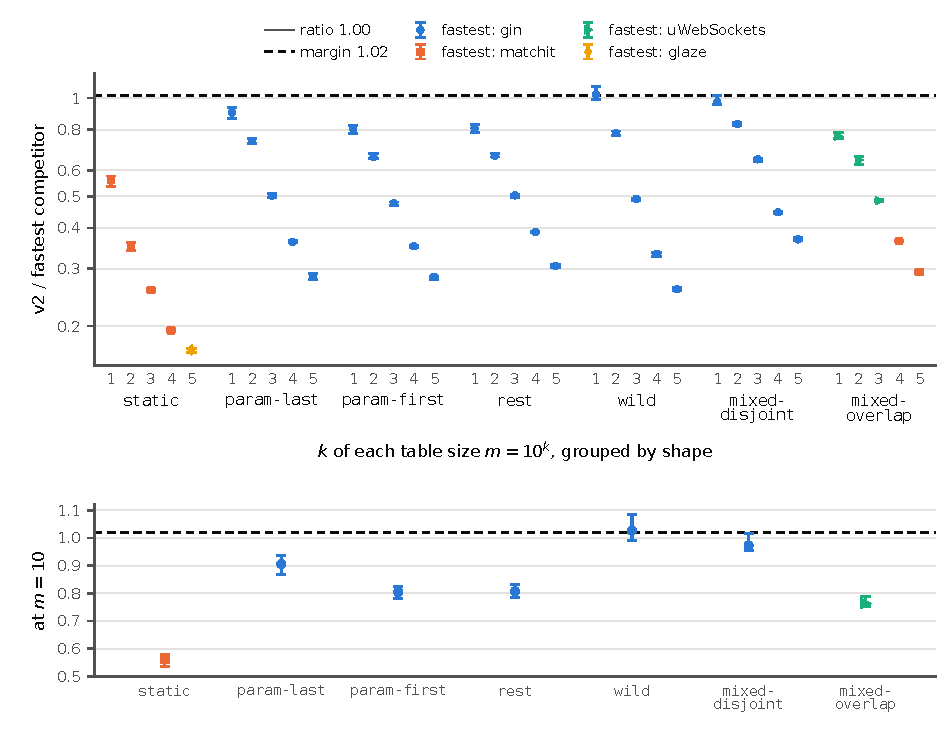
\includegraphics[width=\linewidth]{fig/fig_h1.pdf}
\caption{H1 per cell: v2's time over the fastest competitor's, as the median over the
\RoundTwoReps{} pairs of the per-pair ratio, with its \Level\% BCa interval. Colour and marker name
the fastest competitor. The dashed line is the margin \Margin, and the solid line the ratio
\SupMargin. The upper panel shows every cell on a logarithmic axis. The lower panel shows the cells at
$m=\SizeTen$ on a linear axis, where the two lines are told apart.\label{fig:hone}}
\end{figure}

\begin{table}[htbp]
\caption{H1 per cell. $n$ is the number of competitors in the cell. v2 and F are the medians over
processes of v2's and the fastest competitor's time per lookup. ``Ratio'' is the median of the per-pair
ratios, with its \Level\% BCa interval. $X$ counts the pairs below \Margin. $p_{\mathrm{NI}}$ and
$p_{\mathrm{S}}$ are the larger of the two Holm-adjusted p of non-inferiority and of superiority. NI
and S say whether the cell passes each.\label{tab:hone}}
\begin{adjustwidth}{-\extralength}{0cm}
\centering\footnotesize\setlength{\tabcolsep}{3pt}
\begin{tabular}{@{}llllrrrlrrlrl@{}}
\toprule
\textbf{Shape} & $m$ & \textbf{Fastest} & $n$ & \textbf{v2 (ns)} & \textbf{F (ns)} & \textbf{Ratio} &
\textbf{\Level\% BCa} & $X$ & $p_{\mathrm{NI}}$ & \textbf{NI} & $p_{\mathrm{S}}$ & \textbf{S} \\
\midrule
\HOneRowStaticTen \\ \HOneRowStaticHundred \\ \HOneRowStaticThousand \\ \HOneRowStaticTenThousand \\
\HOneRowStaticHundredThousand \\ \addlinespace
\HOneRowParamLastTen \\ \HOneRowParamLastHundred \\ \HOneRowParamLastThousand \\
\HOneRowParamLastTenThousand \\ \HOneRowParamLastHundredThousand \\ \addlinespace
\HOneRowParamFirstTen \\ \HOneRowParamFirstHundred \\ \HOneRowParamFirstThousand \\
\HOneRowParamFirstTenThousand \\ \HOneRowParamFirstHundredThousand \\ \addlinespace
\HOneRowRestTen \\ \HOneRowRestHundred \\ \HOneRowRestThousand \\ \HOneRowRestTenThousand \\
\HOneRowRestHundredThousand \\ \addlinespace
\HOneRowWildTen \\ \HOneRowWildHundred \\ \HOneRowWildThousand \\ \HOneRowWildTenThousand \\
\HOneRowWildHundredThousand \\ \addlinespace
\HOneRowMixedDisjointTen \\ \HOneRowMixedDisjointHundred \\ \HOneRowMixedDisjointThousand \\
\HOneRowMixedDisjointTenThousand \\ \HOneRowMixedDisjointHundredThousand \\ \addlinespace
\HOneRowMixedOverlapTen \\ \HOneRowMixedOverlapHundred \\ \HOneRowMixedOverlapThousand \\
\HOneRowMixedOverlapTenThousand \\ \HOneRowMixedOverlapHundredThousand \\
\bottomrule
\end{tabular}
\end{adjustwidth}
\end{table}

gin was the fastest competitor in \HOneFastestGinCells{} cells, matchit in
\HOneFastestMatchitCells, uWebSockets in \HOneFastestUWebSocketsCells{} and glaze in
\HOneFastestGlazeCells. The gap grows with the table. On \shape{static}, v2's time rose from
\HOneVtwoNsStaticTen~ns at $m=\SizeTen$ to \HOneVtwoNsStaticHundredThousand~ns at
$m=\SizeHundredThousand$. Over the same sizes, the fastest competitor's rose from
\HOneFastestNsStaticTen~ns to \HOneFastestNsStaticHundredThousand~ns.

\runin{\shape{wild} at $m=\SizeTen$.} This is the one cell that does not pass. Its ratio against
gin is \HOneRatioWildTen, with the interval [\HOneLowWildTen, \HOneHighWildTen]. Only
\HOneSignXWildTen{} of \RoundTwoReps{} pairs are below \Margin, and the Holm-adjusted p is
$\HOnePHolmWildTen$. So the paper claims neither ``not slower'' nor ``faster'' in this cell. The loss is
in a single cell, so the claim narrows at that cell only, as the pre-specification requires.
\shape{wild} passes both tests at every other size. Section~\ref{sec:gin} discusses this cell.

\runin{\shape{mixed-disjoint} at $m=\SizeTen$.} This cell passes non-inferiority and not
superiority. Its ratio against gin is \HOneRatioMixedDisjointTen, with the interval
[\HOneLowMixedDisjointTen, \HOneHighMixedDisjointTen]. Of the sixteen pairs,
\HOneSignXMixedDisjointTen{} are below \Margin, but only \HOneSignXSupMixedDisjointTen{} below
\SupMargin. So v2 is not slower than gin here,
and the paper does not call it faster.

Whether this cell passes depends on the family that Holm's procedure adjusts it in. Before the
repeated check, \HOneAsIsUntested{} cells at $m=\SizeHundredThousand$ could not be tested, because
processes of actix-router were not verified on every query. Each entered Holm with a p of one, and
\HOneAsIsPassed{} of the \HOneAsIsTested{} tested cells passed. This cell's raw sign-test p is
$\HOnePSignRawMixedDisjointTen$ in both analyses. With the untested cells at the bottom of the order,
its Holm multiplier was \HOneHolmMultiplierBeforeMixedDisjointTen, so its adjusted p was
\HOnePSignHolmBeforeMixedDisjointTen, above \Alpha. Once those cells were tested, their p were small. The
cell's multiplier fell to \HOneHolmMultiplierAfterMixedDisjointTen, and its adjusted p to
$\HOnePSignHolmMixedDisjointTen$. Its bootstrap p moved as well, from
\HOnePBootRawBeforeMixedDisjointTen{} to $\HOnePBootRawMixedDisjointTen$ before adjustment, and from
\HOnePBootHolmBeforeMixedDisjointTen{} to $\HOnePBootHolmMixedDisjointTen$ after it. One generator serves the tested cells in the
family's order, so more tested cells change the draws of every later cell. The cell's ratio and
interval do not depend on the family.

\subsection{H2: Work per Lookup}\label{sec:htwo}

H2 \HTwoVerdict. It holds in \HTwoHeld{} of \HTwoJudged{} cells (Table~\ref{tab:htwo}). v2 took fewer
branch misses than the median competitor in every cell, with or without the cut competitors,
\HTwoCutArms. The \HTwoLost{} losses are net instructions against gin, at \HTwoLostCells. At
\shape{param-last}, v2 ran \HTwoVtwoNetParamLastTen{} net instructions per lookup against gin's
\HTwoFastestNetParamLastTen. At \shape{mixed-disjoint}, it ran \HTwoVtwoNetMixedDisjointTen{} against
\HTwoFastestNetMixedDisjointTen. The pre-specification predicted the second loss and not the first.

The memory-side counters per lookup of the losing cells are small for both arms. At
\shape{param-last}, v2 took \HTwoVtwoLOneDParamLastTen{} L1d misses, \HTwoVtwoLTwoParamLastTen{} L2
misses and \HTwoVtwoDtlbParamLastTen{} DTLB misses. gin took \HTwoFastestLOneDParamLastTen,
\HTwoFastestLTwoParamLastTen{} and \HTwoFastestDtlbParamLastTen. At \shape{mixed-disjoint}, v2 took
\HTwoVtwoLOneDMixedDisjointTen, \HTwoVtwoLTwoMixedDisjointTen{} and \HTwoVtwoDtlbMixedDisjointTen,
and gin \HTwoFastestLOneDMixedDisjointTen, \HTwoFastestLTwoMixedDisjointTen{} and
\HTwoFastestDtlbMixedDisjointTen. In both cells v2 still took fewer branch misses than the median
competitor, and by H1 it was not slower than gin.

\begin{table}[htbp]
\caption{H2 per cell: instructions per lookup, net of the null of each arm's own loop and raw, and
branch misses per lookup. ``Median'' is the median competitor's branch misses. The next column leaves
out the competitors whose passes were cut, where any were.\label{tab:htwo}}
\begin{adjustwidth}{-\extralength}{0cm}
\centering\footnotesize\setlength{\tabcolsep}{3.5pt}
\begin{tabular}{@{}lllrrrrrrrl@{}}
\toprule
& & & \multicolumn{2}{c}{\textbf{Net instructions}} & \multicolumn{2}{c}{\textbf{Raw instructions}} &
\multicolumn{3}{c}{\textbf{Branch misses}} & \\
\cmidrule(lr){4-5}\cmidrule(lr){6-7}\cmidrule(lr){8-10}
\textbf{Shape} & $m$ & \textbf{Fastest} & \textbf{v2} & \textbf{Fastest} & \textbf{v2} &
\textbf{Fastest} & \textbf{v2} & \textbf{Median} & \textbf{Uncut} & \textbf{Holds} \\
\midrule
\HTwoRowStaticTen \\ \HTwoRowStaticHundred \\ \HTwoRowStaticThousand \\ \HTwoRowStaticTenThousand \\
\HTwoRowStaticHundredThousand \\ \addlinespace
\HTwoRowParamLastTen \\ \HTwoRowParamLastHundred \\ \HTwoRowParamLastThousand \\
\HTwoRowParamLastTenThousand \\ \HTwoRowParamLastHundredThousand \\ \addlinespace
\HTwoRowParamFirstTen \\ \HTwoRowParamFirstHundred \\ \HTwoRowParamFirstThousand \\
\HTwoRowParamFirstTenThousand \\ \HTwoRowParamFirstHundredThousand \\ \addlinespace
\HTwoRowRestTen \\ \HTwoRowRestHundred \\ \HTwoRowRestThousand \\ \HTwoRowRestTenThousand \\
\HTwoRowRestHundredThousand \\ \addlinespace
\HTwoRowWildTen \\ \HTwoRowWildHundred \\ \HTwoRowWildThousand \\ \HTwoRowWildTenThousand \\
\HTwoRowWildHundredThousand \\ \addlinespace
\HTwoRowMixedDisjointTen \\ \HTwoRowMixedDisjointHundred \\ \HTwoRowMixedDisjointThousand \\
\HTwoRowMixedDisjointTenThousand \\ \HTwoRowMixedDisjointHundredThousand \\ \addlinespace
\HTwoRowMixedOverlapTen \\ \HTwoRowMixedOverlapHundred \\ \HTwoRowMixedOverlapThousand \\
\HTwoRowMixedOverlapTenThousand \\ \HTwoRowMixedOverlapHundredThousand \\
\bottomrule
\end{tabular}
\end{adjustwidth}
\end{table}

\subsection{H3: No Allocation}\label{sec:hthree}

H3 \HThreeVerdict. In all \HThreeProcesses{} processes of v2 over the \HOneCells{} cells, a lookup made
no heap allocation. The compile-time arm, in its \HThreeCtProcesses{} processes, and the ablation arm,
in its \HThreeAblationProcesses, made none either.

\subsection{H4: Build Time and Memory}\label{sec:hfour}

H4 \HFourVerdict. It fails in \HFourLost{} cells, all on build time: \shape{static} and
\shape{param-first} at $m=\SizeTenThousand$ and \SizeHundredThousand. There v2's build took
\HFourLostRatioMin{} to \HFourLostRatioMax{} times the median competitor's (Table~\ref{tab:hfour}).
The other two bounds hold in every cell. v2's slowest build at $m=\SizeHundredThousand$ took
\HFourBuildMaxMs~ms, below \BuildLimitSeconds~s. Its table held \HFourHeapRatioMin{} to
\HFourHeapRatioMax{} times the heap bytes of the smallest competitor, within the factor
\HeapFactor. As pre-specified, H4's claim is not made.

\begin{table}[htbp]
\caption{H4 per cell. Build times are medians over processes of each process's median build, in
microseconds. ``Median'' is the median competitor's build time. Heap bytes are those the built table
holds. ``Smallest'' is the competitor with the fewest.\label{tab:hfour}}
\begin{adjustwidth}{-\extralength}{0cm}
\centering\footnotesize\setlength{\tabcolsep}{4pt}
\begin{tabular}{@{}llrrrrllll@{}}
\toprule
& & \multicolumn{2}{c}{\textbf{Build ($\mu$s)}} & \multicolumn{3}{c}{\textbf{Heap bytes}} &
\multicolumn{3}{c}{\textbf{Holds}} \\
\cmidrule(lr){3-4}\cmidrule(lr){5-7}\cmidrule(lr){8-10}
\textbf{Shape} & $m$ & \textbf{v2} & \textbf{Median} & \textbf{v2} & \textbf{Smallest} & & \textbf{Build} &
\textbf{Heap} & \textbf{Cell} \\
\midrule
\HFourRowStaticTen \\ \HFourRowStaticHundred \\ \HFourRowStaticThousand \\ \HFourRowStaticTenThousand \\
\HFourRowStaticHundredThousand \\ \addlinespace
\HFourRowParamLastTen \\ \HFourRowParamLastHundred \\ \HFourRowParamLastThousand \\
\HFourRowParamLastTenThousand \\ \HFourRowParamLastHundredThousand \\ \addlinespace
\HFourRowParamFirstTen \\ \HFourRowParamFirstHundred \\ \HFourRowParamFirstThousand \\
\HFourRowParamFirstTenThousand \\ \HFourRowParamFirstHundredThousand \\ \addlinespace
\HFourRowRestTen \\ \HFourRowRestHundred \\ \HFourRowRestThousand \\ \HFourRowRestTenThousand \\
\HFourRowRestHundredThousand \\ \addlinespace
\HFourRowWildTen \\ \HFourRowWildHundred \\ \HFourRowWildThousand \\ \HFourRowWildTenThousand \\
\HFourRowWildHundredThousand \\ \addlinespace
\HFourRowMixedDisjointTen \\ \HFourRowMixedDisjointHundred \\ \HFourRowMixedDisjointThousand \\
\HFourRowMixedDisjointTenThousand \\ \HFourRowMixedDisjointHundredThousand \\ \addlinespace
\HFourRowMixedOverlapTen \\ \HFourRowMixedOverlapHundred \\ \HFourRowMixedOverlapThousand \\
\HFourRowMixedOverlapTenThousand \\ \HFourRowMixedOverlapHundredThousand \\
\bottomrule
\end{tabular}
\end{adjustwidth}
\end{table}

\subsection{H5: Checked When Compiled, Correct When Run}\label{sec:hfive}

H5 holds in all three parts. (a) RegexMatcher's suite at the measured commit holds the \NegCases{}
negative-compilation cases, one test each. Each expects the compilation to fail and checks that the
diagnostic names the reason. Under each of the three sanitizers on L, all \HFiveATests{} tests of the
suite passed. (b) v2 answered all \HFiveBLookups{} lookups of the probes as the rules require.
Table~\ref{tab:probes} shows every arm. v1 behind its wrapper fails two probes; this decides
nothing. Of the competitors, only matchit and path-tree pass every probe,
as v2 does. (c) The minimal server's suite checks that the GET route serves HEAD on a path that only
GET routes match, without content. It also checks that a HEAD route wins over that fallback, and that
Allow lists HEAD whenever it lists GET. The suite passed under each of the three sanitizers on L.

\begin{table}[htbp]
\caption{The probes of the path rules on every arm. S$\to$P and P$\to$S register a literal route
before a parameter route and after it. ``pchar'' sends every pchar in a parameter, ``raw'' a path
that differs only in the case of a percent escape. ``catch-all'' and ``empty'' test the rules on
remainders and empty segments, ``slash'' a trailing slash, and 405 a path of another method.
$\checkmark$: every lookup right; $\times$: at least one wrong; $\circ$: the arm refused the probe's
routes.\label{tab:probes}}
\centering\footnotesize\setlength{\tabcolsep}{4pt}
\begin{tabular}{@{}lcccccccc@{}}
\toprule
\textbf{Arm} & S$\to$P & P$\to$S & pchar & raw & catch-all & empty & slash & 405 \\
\midrule
\ProbeArms
\bottomrule
\end{tabular}
\end{table}

\subsection{H6: The Client Sees the Difference}\label{sec:hsix}

H6 holds. Part (a) \HSixAVerdict{} in \HSixAHeld{} of \HSixCells{} cells, and part (b) \HSixBVerdict{}
in \HSixBHeld{} of \HSixCells{} (Table~\ref{tab:hsix}). Every cell stopped at \HSixMinPairs{} valid
pairs, and none of the \HSixWindows{} windows was invalid. With v2 the server answered
\HSixVtwoRpsMin{} to \HSixVtwoRpsMax{} requests per second in every cell. At $m=\SizeTen$ the lower
bounds of the ratio over v1 ranged from \HSixLowMinTen{} to \HSixLowMaxTen. At \shape{rest} with
$m=\SizeTenThousand$, v1's lookup dominated its server's time, and the ratio was
\HSixRatioRestTenThousand. There v1's lookup time in the main grid rests on a prefix of
\HSixVOnePrefixRestTenThousand{} of the \RingSize{} queries, as the pre-specification allows.

The lower bounds of the carry-over ranged from \HSixCarryLowMin{} to \HSixCarryLowMax, all above
\CarryBound. The null arm took \HSixNullUsMin{} to \HSixNullUsMax~$\mu$s per request. The measured
ratio was \HSixPredMin{} to \HSixPredMax{} times the ratio that the lookup times predict. In every
cell every pair favoured v2 and carried at least \CarryBound, so each sign test gives \HSixSignMinP.
H6 compares v2 with v1 in the paper's own server. It says nothing about the competitors, nor about a
full framework.

\begin{table}[htbp]
\caption{H6 per cell, over loopback with the minimal server. Rates are the medians over pairs, in
requests per second. ``Low'' is the lower bound of the \Level\% BCa interval. $D_{T0}$ and
$D_{\mathrm{meas}}$ are in ns per request. The last column is the measured ratio over the predicted
one.\label{tab:hsix}}
\begin{adjustwidth}{-\extralength}{0cm}
\centering\footnotesize\setlength{\tabcolsep}{3.5pt}
\begin{tabular}{@{}llrrrrrrrrrr@{}}
\toprule
\textbf{Shape} & $m$ & \textbf{Pairs} & \textbf{v1} & \textbf{v2} & \textbf{v2/v1} & \textbf{Low} &
$D_{T0}$ & $D_{\mathrm{meas}}$ & $D_{\mathrm{meas}}/D_{T0}$ & \textbf{Low} & \textbf{Meas./pred.} \\
\midrule
\HSixRowStaticTen \\ \HSixRowParamLastTen \\ \HSixRowParamFirstTen \\ \HSixRowRestTen \\
\HSixRowWildTen \\ \HSixRowMixedDisjointTen \\ \HSixRowMixedOverlapTen \\ \addlinespace
\HSixRowRestTenThousand \\ \HSixRowParamLastTenThousand \\
\bottomrule
\end{tabular}
\end{adjustwidth}
\end{table}

\subsection{H7: A Table Built at Compile Time}\label{sec:hseven}

H7 \HSevenVerdict. The compile-time table passed its per-cell test in \HSevenHeld{} of
\HSevenCells{} cells, and the rule needs all of them (Figure~\ref{fig:hseven} and
Table~\ref{tab:hseven}). The bootstrap passed in all \HSevenHeldBoot{} cells, and the largest upper
bound was \HSevenMaxHigh. The sign test failed in one cell, \HSevenLostCell. There only
\HSevenLostSignX{} pairs are below \Margin, where \HSevenSignNeed{} are needed, and p is
\HSevenLostPSign. As pre-specified, H7's claim is not made.

In that cell the compile-time table is measurably slower, by a small margin. Its median ratio is
\HSevenLostRatio, and its \Level\% BCa interval, [\HSevenLostLow, \HSevenLostHigh], lies wholly above
one. Of the sixteen pairs, \HSevenLostAboveOne{} are above one and \HSevenLostAboveMargin{} reach the
margin, where the rule allows \HSevenAllowedAbove. One of them, at table seed \HSevenLostSeed,
has the ratio \HSevenLostMaxPair. There the compile-time table took \HSevenLostSeedCyclesCt{} cycles
per lookup against \HSevenLostSeedCyclesRt, with equal instructions. The largest ratio of the other
pairs is \HSevenLostOthersMax. This pair is an observation only, and it does not explain the cell.

\runin{The heap-block follow-up.} For such a cell, the pre-specification named an exploratory run
with the compile-time table copied into a heap block, to test whether the table's place in memory is
the cause. It was made after the main grid, not in the frozen order, and it decides nothing. One
binary held the run-time table, the compile-time table and the heap copy, on the same
\ExCtHeapPairs{} pairs. There table seed \ExCtHeapSeed{} no longer stood apart. Its compile-time table
took \ExCtHeapCtRtSeed{} of the run-time table's time, and its heap copy \ExCtHeapHeapRtSeed. Over the
other pairs, the heap copy took \ExCtHeapHeapRtOthersMin{} to \ExCtHeapHeapRtOthersMax{} of the
run-time table's time, with the median \ExCtHeapHeapRtOthersMedian.

Single slow pairs appeared again, at other seeds and in each arm. The compile-time table took
\ExCtHeapCtRtOthersMax{} of the run-time table's time at table seed \ExCtHeapCtRtOthersMaxSeed. The
heap copy took \ExCtHeapHeapRtOthersMax{} at table seed \ExCtHeapHeapRtOthersMaxSeed. The run-time
table ran \ExCtHeapCyclesRtMax{} cycles per lookup at table seed \ExCtHeapCyclesRtMaxSeed, against
its median of \ExCtHeapCyclesRtMedian. The heap copy took as many L1d misses per lookup as the
run-time table, \ExCtHeapLOneDHeapMedian{} against \ExCtHeapLOneDRtMedian, and the compile-time table
fewer, \ExCtHeapLOneDCtMedian, while their times stayed alike. So a slow pair followed neither the
table seed nor the table's place in memory. The run does not identify what slowed those pairs.

\begin{figure}[htbp]
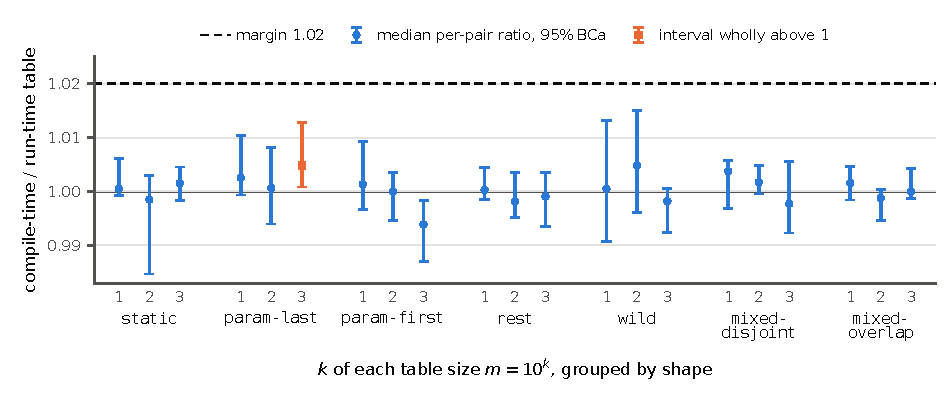
\includegraphics[width=\linewidth]{fig/fig_h7.pdf}
\caption{H7 per cell: the compile-time table's time over the run-time table's, as the median of the
per-pair ratios, with its \Level\% BCa interval. A square marks a cell whose whole interval lies above
one. The dashed line is the margin \Margin.\label{fig:hseven}}
\end{figure}

\begin{table}[htbp]
\caption{H7 per cell. CT and RT are the medians over processes of the compile-time and run-time
tables' times per lookup. ``Upper'' is the upper bound of the \Level\% BCa interval. $X$ counts the
pairs below \Margin, and $p$ is the exact sign test's.\label{tab:hseven}}
\centering\footnotesize\setlength{\tabcolsep}{3.5pt}
\begin{tabular}{@{}llrrrrrrlll@{}}
\toprule
\textbf{Shape} & $m$ & \textbf{CT (ns)} & \textbf{RT (ns)} & \textbf{Ratio} & \textbf{Upper} & $X$ & $p$ &
\textbf{Boot.} & \textbf{Sign} & \textbf{Holds} \\
\midrule
\HSevenRowStaticTen \\ \HSevenRowStaticHundred \\ \HSevenRowStaticThousand \\ \addlinespace
\HSevenRowParamLastTen \\ \HSevenRowParamLastHundred \\ \HSevenRowParamLastThousand \\ \addlinespace
\HSevenRowParamFirstTen \\ \HSevenRowParamFirstHundred \\ \HSevenRowParamFirstThousand \\ \addlinespace
\HSevenRowRestTen \\ \HSevenRowRestHundred \\ \HSevenRowRestThousand \\ \addlinespace
\HSevenRowWildTen \\ \HSevenRowWildHundred \\ \HSevenRowWildThousand \\ \addlinespace
\HSevenRowMixedDisjointTen \\ \HSevenRowMixedDisjointHundred \\ \HSevenRowMixedDisjointThousand \\
\addlinespace
\HSevenRowMixedOverlapTen \\ \HSevenRowMixedOverlapHundred \\ \HSevenRowMixedOverlapThousand \\
\bottomrule
\end{tabular}
\end{table}

\runin{The costs of a compile-time table.} Table~\ref{tab:costs} reports what the tables cost the
compilers. On L, clang \ClangVersion{} compiled each of the \CostTables{} tables in a fresh build, one
job at a time, at the native flags. These are the \CostTablesPerSize{} tables of each size, from the
sixteen table seeds of the run and one more, and the GitHub table. A table's object size is the sum of
its sections named \texttt{.text*}, \texttt{.rodata*}, \texttt{.data.rel.ro*}, the other
\texttt{.data*}, and \texttt{.bss*}. Each object file is \CostPadMin{} to \CostPadMax{} bytes larger.
The page alignment of the table pads the file, without adding memory that the lookup touches.

Clang's need of constant-evaluation steps was measured for the tables of table seed \TableSeedFirst{}
and for the GitHub table. The search doubles the budget from \StepsStart{} steps, so each value is the
smallest budget tried under which a table compiled. Every table of \SizeThousand{} routes compiled
within \ClangNeedMax{} steps and failed at \ClangThousandFailSteps. The budget of \ConstexprSteps{} is
twice the largest of these. On W, an \HostWCpu{} (\HostWArch), MSVC \MsvcVersion{} compiled the same
\MsvcTables{} tables one at a time, with the flags of RegexMatcher's own test of compile-time tables.
Its search starts at \StepsStart{} steps and multiplies by four. At \SizeThousand{} routes every table
crashed the compiler at \MsvcCrashSteps{} steps and failed with the budget error at
\MsvcBudgetFailSteps. Each then compiled at the budget found by halving the last factor of four,
shown in Table~\ref{tab:costs}. At the harness's budget, the compiles of those tables took
\MsvcPeakMinMiB{} to \MsvcPeakMaxMiB~MiB of memory. These are compiler measurements of code that never
runs, so they need no sanitizer record.

\begin{table}[htbp]
\caption{The costs of the compile-time tables: clang on L at the native flags, and MSVC on W, one
compile at a time. Clang's compile time and object size cover every table of a size. The steps and
MSVC's columns cover the tables of table seed \TableSeedFirst{} at each size, and the GitHub table.
Steps are the smallest budget of constant evaluation tried under which a table compiled. Peak memory
is the compiler's peak committed memory at the harness's budget.\label{tab:costs}}
\begin{adjustwidth}{-\extralength}{0cm}
\centering\footnotesize\setlength{\tabcolsep}{4pt}
\begin{tabular}{@{}lrrrrrrr@{}}
\toprule
& & \multicolumn{3}{c}{\textbf{Clang on L}} & \multicolumn{3}{c}{\textbf{MSVC on W}} \\
\cmidrule(lr){3-5}\cmidrule(lr){6-8}
$m$ & \textbf{Tables} & \textbf{Compile (s)} & \textbf{Object (B)} & \textbf{Steps} & \textbf{Steps} &
\textbf{Peak (MiB)} & \textbf{Object file (B)} \\
\midrule
\CostRowTen \\ \CostRowHundred \\ \CostRowThousand \\ \CostRowGithub \\
\bottomrule
\end{tabular}
\end{adjustwidth}
\end{table}

\subsection{Exploratory Runs}\label{sec:exploratory}

The exploratory runs decide nothing and have no intervals (Table~\ref{tab:explore}). On the GitHub
table, v2 took \ExGithubRatio{} of the time of the fastest competitor, \ExGithubFastest, over
\ExGithubPairs{} pairs. It ran \ExGithubVtwoNet{} net instructions per lookup against
\ExGithubFastestNet. With half the queries missing, v2's ratio to the fastest competitor ranged from
\ExMissRatioMin, at \ExMissRatioMinCell, to \ExMissRatioMax, at \ExMissRatioMaxCell. No cell was above
one. v2 ran more net instructions than the fastest competitor in \ExMissNetAbove{} of those cells, all
at $m=\SizeTen$.

Long literals did not close the gap. Their ratios ran from \ExVocabRatioMin{} to \ExVocabRatioMax, and
v2 ran fewer net instructions in all \ExVocabCells{} cells. The Zipf ring gave \ExZipfRatioMin{} to
\ExZipfRatioMax, again with fewer net instructions in every cell. Without decoys, gin holds the
\shape{mixed-overlap} tables, and v2's ratio ran from \ExNoDecoyRatioMin{} to \ExNoDecoyRatioMax{} up
to $m=\SizeTenThousand$. At $m=\ExNoDecoyFailedSize$ the analysis failed that cell. There gin and
Boost.URL agreed in \ExNoDecoyFailOk{} of \RoundTwoReps{} processes and differed as declared in the
others. An arm must agree in all of a cell's processes or in none.

\begin{table}[htbp]
\caption{The exploratory runs, against the fastest competitor of each cell. $R$ is the number of pairs
per cell. ``v2 / fastest'' gives the range over cells of the median over pairs of the per-pair ratio.
The last column counts the cells where v2 ran more net instructions than the fastest
competitor.\label{tab:explore}}
\centering\footnotesize
\begin{tabular}{@{}lrrll@{}}
\toprule
\textbf{Run} & \textbf{Cells} & $R$ & \textbf{v2 / fastest} & \textbf{More instructions} \\
\midrule
GitHub table & one & \ExGithubPairs & \ExGithubRatio & none \\
\ExMissRow \\ \ExVocabRow \\ \ExZipfRow \\ \ExNoDecoyRow \\
\bottomrule
\end{tabular}
\end{table}

The ablation arm shows what the rework of Section~\ref{sec:rework} changed. Against it, v2's lookup time
ranged from \AbTimeMin{} to \AbTimeMax{} of the ablation arm's over the \AbCells{} cells, and its net
instructions were equal (\AbInsnMin). The build took \AbBuildMin{} to \AbBuildMax{} of the ablation
arm's time, and the table's heap bytes were \AbHeapMin{} to \AbHeapMax{} of its bytes.
Appendix~\ref{app:ablation} gives every cell. The rework improved the build time and the heap, and left
the lookup unchanged.

\section{Discussion}\label{sec:discussion}

\subsection{What the Results Support}

In the setting of Section~\ref{sec:host}, v2 is the fastest of the route matchers measured here in
\HOneSuperior{} of \HOneCells{} cells, and not slower in one more. ``Fastest'' is said of a cell only
against the competitors that take part in it. The competitors left out are named with their reasons
in Section~\ref{sec:run}, and the paper does not claim that they are slower.

The advantage grows with the table. v2's work per lookup barely depends on $m$. On \shape{static} it
ran \HTwoVtwoNetStaticTen{} net instructions per lookup at $m=\SizeTen$ and
\HTwoVtwoNetStaticHundredThousand{} at $m=\SizeHundredThousand$, while the fastest competitor's count
rose from \HTwoFastestNetStaticTen{} to \HTwoFastestNetStaticHundredThousand. A walk over path
segments takes one step per segment, so its length follows the depth of the route, not the number of
routes. The width of a node matters only through its scan of up to \VTwoLinearEdges{} literal
children, or one probe of their hashed slots. In every cell, v2 also took fewer branch misses than
the median competitor.

\subsection{Small Tables Against gin}\label{sec:gin}

Every loss or partial result of v2 in the lookup comparison sits at $m=\SizeTen$ and against gin.
These are the \HTwoLost{} H2 losses, the one cell that does not pass H1, and the one cell that passes
non-inferiority only. With ten routes, first words rarely repeat, so most nodes below the root have
one child. A node of gin's tree compares its whole prefix at once, while v2 takes one step per
segment. The development round attributed the instruction loss at \shape{mixed-disjoint} to this
difference. The rework tried to remove it with chains, and its rules rejected every attempt
(Section~\ref{sec:rework}).

An instruction count is not a time, however. At \shape{param-last} with $m=\SizeTen$, v2 ran more net
instructions than gin and was still faster, with the ratio \HOneRatioParamLastTen. Part of v2's count
is the harness's adapter, which copies the captured values into the harness's own structure and folds
them. gin folds its values inside Go, and its null pass does not. Appendix~\ref{app:lookup} lists
these differences between the arms. We kept them, because removing them would change the harness for
every arm.

At \shape{wild} with $m=\SizeTen$, the development builds favoured v2. The run differs from those
builds in the instruction set that every arm targets and in the build level of the Go arms. Both are
candidate causes of the change in this cell, and neither was tested.

\subsection{Build Time and the Compile-Time Table}

The rework cut v2's build to \AbBuildMin{} to \AbBuildMax{} of the pre-release's time and reduced its
heap. It was not enough in \HFourLostBuild{} cells, at \shape{static} and \shape{param-first} with
$m=\SizeTenThousand$ and \SizeHundredThousand. We did not profile what remains of the build there. A
server builds its table once at start, and v2's slowest build of the largest tables took
\HFourBuildMaxMs~ms. As pre-specified, H4's claim is not made.

The compile-time table passed its per-cell test in \HSevenHeld{} of \HSevenCells{} cells. The rule
needs all of them, so H7 does not hold. The one cell that fails has \HSevenLostAboveMargin{} pairs at
or above the margin, where the rule allows \HSevenAllowedAbove, and its interval lies wholly above
one. One of them, at table seed \HSevenLostSeed, ran more cycles with the same instructions. The
rework had already given both tables one layout. What remains between them includes where the table
lies, in the binary or on the heap, and where the code lies. The pre-specified run with a heap copy,
made afterwards, found single slow pairs at other seeds and in each arm. Neither the table seed nor
the table's place in memory explains the cell, and its cause stays open. Zero-overhead abstraction is therefore not established
here for compile-time tables~\cite{stroustrup2012foundations}.

The costs set a practical limit. A compile-time table of \SizeThousand{} routes took
\ClangThousandCompileMin{} to \ClangThousandCompileMax~s to compile with clang. With MSVC it took
\MsvcPeakMinMiB{} to \MsvcPeakMaxMiB~MiB of memory, and MSVC crashed under the smallest budget of its
search. A compile-time table is cheap at \SizeTen{} and \SizeHundred{} routes and expensive at
\SizeThousand.

\subsection{End to End}

The lookup difference against v1 reached the client in every cell of H6. In the minimal server the
null router's time per request was about \HSixNullUsMin~$\mu$s, so routing is a visible share of a
request in a server this lean. The measured ratio stayed within \HSixPredMin{} to \HSixPredMax{} of
the ratio that the lookup times predict. The share would be smaller in a full framework with more
work per request.

\subsection{Threats to Validity}\label{sec:threats}

\begin{itemize}
\item \textbf{One processor model and one core.} Every time comes from one core of one \HostLArch{}
processor. Another microarchitecture may rank close cells differently, above all the cells at
$m=\SizeTen$ against gin.
\item \textbf{One compiler per language.} C and C++ were compiled by clang only, Rust by rustc and Go by
its own toolchain. GCC and MSVC builds were not timed. MSVC appears only in the costs of compile-time
tables.
\item \textbf{The native instruction set.} Every arm was built for L's own processor. A generic build
would give other code and other times, which may matter most for the small tables against gin.
\item \textbf{Loopback for H6.} The end-to-end run used loopback, one server core and one request in
flight per connection. A network, more cores or pipelining would change the share of routing.
\item \textbf{The minimal server.} It parses, routes and answers a fixed body. A full framework adds
work per request, which dilutes the difference between routers.
\item \textbf{Development on the same host.} The engineering of v2 ran on L, on other seeds. The run's
seeds were held out, but the design choices may still suit L's microarchitecture better than others.
\item \textbf{The Drogon transcription.} Drogon's router needs a running application, so its lookup was
transcribed into the harness from its source. The file's hash and line ranges are pinned. A
transcription can still differ from the router as Drogon runs it.
\item \textbf{The gin shim.} gin's tree is vendored unchanged, but the parts of gin's engine that a
lookup uses are reproduced in a small shim. They are the reset of the context, the method's tree and
the search in gin's default configuration. chi's arm uses a similar shim of its multiplexer. A shim
can differ from the engine it stands for.
\item \textbf{The repeated ring.} Every timed pass repeats the same \RingSize{} queries. Predictors and
caches learn the ring, and a large table's hot part is at most the ring's routes. Real traffic, with
more distinct paths, may favour other structures. The Zipf and miss-heavy rings explore two departures
only.
\item \textbf{Foreign-function boundaries.} The Rust arms are called through one C function per lookup,
and the Go arms run their timed loops inside Go, entered through cgo. Their nulls remove the loops, not
every cost of the boundary.
\item \textbf{The cut for slow arms.} A competitor whose passes ran on a prefix of the ring has
optimistic times and counters. None was the fastest competitor of an H1 cell, but the cut competitors
enter the median of H2's branch misses, which Table~\ref{tab:htwo} gives with and without them.
\end{itemize}

\section{Conclusions}\label{sec:conclusions}

We surveyed the route matchers of sixteen routers in C, C++, Rust and Go, and reworked the author's
RegexMatcher library into a route matcher, RegexMatcher~v2. Its lookup walks a trie of path segments
stored in flat arrays, answers literal-only methods from an exact-match table, and never allocates.
Its front end checks patterns, handler signatures and duplicate routes when the program compiles.

Under hypotheses pre-specified before the run, and in the setting of Section~\ref{sec:host}, v2 was
faster than the fastest competitor in \HOneSuperior{} of \HOneCells{} cells. It was not slower in
one more. At the \shape{wild} shape with \SizeTen{} routes, neither claim holds against gin. v2 ran more
instructions than gin in \HTwoLost{} cells of \SizeTen{} routes. It built its table more slowly than
the median competitor in \HFourLostBuild{} cells with large tables. The compile-time table passed its
per-cell test in \HSevenHeld{} of \HSevenCells{} cells; the rule needs all, so H7 does not hold. No
lookup of v2 allocated, every probe of the path rules passed, and the compile-time checks rejected
every malformed case. In a minimal server, the lookup difference against v1 reached the client in
every cell.

Three questions remain open. The first is whether the results hold on other processors and with other
compilers, above all for small tables. The second is why the compile-time table was slower at
\HSevenLostCell. The pre-specified run with a heap copy did not tie the slow pairs to the table's
place in memory, and it cannot rule out the placement of code. The third is what remains of the build
time for large literal tables.


\vspace{6pt}

\supplementary{The following supporting information can be downloaded at
\PaperRepoURL: Table S1, every arm in every cell of
the main grid. Table S1 gives each value as the median over the arm's processes. It is the file
\texttt{results/round2/all\_arms.csv} of the paper's repository. Its columns are the arm's role, its processes and their statuses, and whether it takes part in the
cell, with the reason when it does not. They also hold the time per lookup, the raw and net
instructions, the branch misses, the cycles, and the L1d, L2 and DTLB misses. The allocations per
lookup, the build time, the bytes allocated by the build and the heap bytes of the table follow.
The latency percentiles and, for the Go arms, the cost of an empty call across cgo complete them.}

\authorcontributions{Conceptualization, A.I.T.; methodology, A.I.T.; software, A.I.T.;
validation, A.I.T.; formal analysis, A.I.T.; investigation, A.I.T.; resources, A.I.T.; data
curation, A.I.T.; writing, original draft preparation, A.I.T.; writing, review and editing,
A.I.T.; visualization, A.I.T.; supervision, A.I.T.; project administration, A.I.T.; funding
acquisition, A.I.T. The author has read and agreed to the published version of the manuscript.}

\funding{The publication of this paper was financially supported by the scientific research
sector of the Technical University of Sofia.}

\institutionalreview{Not applicable.}

\informedconsent{Not applicable.}

\dataavailability{The paper's repository, \PaperRepoURL, holds the harness and the minimal server at
commit \hex{\RbenchPublicCommitFull}, with the analysis, the pre-specification and the derived
tables. It also holds the sources of the T1 tools that ran H6 (\texttt{lab/t1/}). The raw runs are
the assets of its release \DataRelease{} (\DataReleaseURL), and \texttt{results/round2/archives.sha256}
lists them. The raw main grid is \hex{\ArchiveMain}, SHA-256 \hex{\ArchiveMainSha}. The repeated
check of its answers is \hex{\ArchiveVerify}, SHA-256 \hex{\ArchiveVerifySha}. The clang costs of
the compile-time tables are \hex{\ArchiveCt}, SHA-256 \hex{\ArchiveCtSha}. The MSVC costs are
\hex{\ArchiveMsvc}, SHA-256 \hex{\ArchiveMsvcSha}. The end-to-end run is \hex{\ArchiveHSix}, SHA-256
\hex{\ArchiveHSixSha}. The exploratory runs are \hex{\ArchiveExGithub}, SHA-256
\hex{\ArchiveExGithubSha}, and \hex{\ArchiveExMiss}, SHA-256 \hex{\ArchiveExMissSha}. They are also
\hex{\ArchiveExVocab}, SHA-256 \hex{\ArchiveExVocabSha}; \hex{\ArchiveExZipf}, SHA-256
\hex{\ArchiveExZipfSha}; and \hex{\ArchiveExNoDecoy}, SHA-256 \hex{\ArchiveExNoDecoySha}. The
heap-block follow-up of H7 is \hex{\ArchiveCtHeap}, SHA-256 \hex{\ArchiveCtHeapSha}. The sanitizer
records that gated the harness and the server, those made later for the published commit, and those
behind H5(a) and H5(c) are in \RecordsDir{} of the repository. Each record names the SHA-256 of an archive of its logs, which are not published.
RegexMatcher~v2 is commit \hex{\RegexMatcherCommitFull}. It is available at \RegexMatcherURL{} in
release \RegexMatcherRelease. \ForAlex{the DOIs of the paper's repository and of its release
\DataRelease, which need Alex's account (for example a Zenodo archive of the release).}}

\acknowledgments{The author would like to thank the scientific research sector of the Technical University of Sofia for financial support for publishing the present paper.}

\conflictsofinterest{The author declares no conflicts of interest. The funder had no role in the
design of the study; in the collection, analyses, or interpretation of data; in the writing of
the manuscript; or in the decision to publish the results.}

\appendixtitles{yes}
\appendixstart
\appendix
\section[\appendixname~\thesection]{What Each Arm's Timed Lookup Includes}\label{app:lookup}

For every arm, the timed loop calls the arm's own pass if it has one, as the Go arms do. Otherwise it
runs the harness's loop over the compact copy of the ring. The loop adds each route number, and each
captured value's length and first byte, to a sink that the compiler cannot remove. For an arm without
a 405 of its own, a ``no route'' answer starts a lookup of the same path under every other method
that has routes. Any hit makes the answer 405. On the all-hit rings of the grid, that fallback runs
only after a wrong answer, but its test runs on every lookup. The allocation pass and the latency
samples call each lookup through the harness, so a Go arm's latency includes one call across cgo.

``Index'' in Table~\ref{tab:lookup} means that the harness passes the method as a number and the
adapter indexes one router per method. ``String'' means that the router takes the method's name.

\begin{table}[htbp]
\caption{The timed call of each arm. ``Loop'' is the loop that times the arm, and ``null'' the null
that H2 subtracts.\label{tab:lookup}}
\begin{adjustwidth}{-\extralength}{0cm}
\centering\scriptsize\setlength{\tabcolsep}{3pt}
\begin{tabularx}{\fulllength}{@{}l X l X l l@{}}
\toprule
\textbf{Arm} & \textbf{Timed call} & \textbf{Method} & \textbf{Captured values} & \textbf{405} &
\textbf{Loop; null} \\
\midrule
\arm{regexmatcher-v2} & \FindVtwo, out of line, which calls \texttt{matcher::route::find} & index & views into the path & its own & harness; \arm{null} \\
\arm{regexmatcher-v2-ct} & the same, on the compile-time table & index & views & its own & harness; \arm{null} \\
\AblationArm & the pre-release's lookup, out of line & index & views & its own & harness; \arm{null} \\
\arm{regexmatcher-v1} & the wrapper's match, which calls v1's matching with groups & index & offsets; a new result vector per call & harness & harness; \NullNoFive \\
radix, hash, regex & the harness's lookups & index & views (hash: none) & harness & harness; \NullNoFive \\
Crow & \texttt{crow::Trie::find} & index & copied into strings; views of them & harness & harness; \NullNoFive \\
Oat++ & \texttt{Router::getRoute} & index & views; the tail copied into a string & harness & harness; \NullNoFive \\
Boost.URL & \texttt{parse\_path}, then the router's \texttt{find} & index & views & harness & harness; \NullNoFive \\
r3 & one match entry created, matched and freed per lookup & a bit in the entry & views & harness & harness; \NullNoFive \\
Drogon & the transcribed lookup: a lower-cased copy, two maps, then a regular expression per route & index & a new vector of strings per match & harness & harness; \NullNoFive \\
Pistache & \texttt{sanitizeResource}, then \texttt{findRoute} & index & copies, its only public read & harness & harness; \NullNoFive \\
matchit & \texttt{Router::at} behind one C call & index & offsets & harness & harness; \NullNoFive \\
actix-router & \texttt{Path::set}, then \texttt{Router::recognize}, behind one C call & index & offsets, not decoded & harness & harness; \NullNoFive \\
path-tree & \texttt{PathTree::find} behind one C call & index & offsets & harness & harness; \NullNoFive \\
uWebSockets & \texttt{HttpRouter::route}; the handler stores the route & string & views; none for a catch-all & harness & harness; \NullNoFive \\
glaze & \texttt{route\_table::match} & a switch & decoded strings in a map; one find per name & harness & harness; \NullNoFive \\
cpp-httplib & the request's path assigned, then the method's matchers in order & index & named values copied; groups as views & harness & harness; \NullNoFive \\
httprouter & \texttt{Router.Lookup}, then the handler, in Go & string & offsets & the harness's rule, in Go & its own; its own \\
gin & the vendored tree's search, then the handlers, in Go & string & offsets; values after a return copied & the harness's rule, in Go & its own; its own \\
net/http & \texttt{ServeMux.ServeHTTP} on one reused request, in Go & string & the handler copies each value & its own & its own; its own \\
chi & the context reset, the method map, the tree search, then the handler, in Go & string & offsets & the harness's rule, in Go & its own; its own \\
\bottomrule
\end{tabularx}
\end{adjustwidth}
\end{table}

What remains unequal is stated rather than removed, because removing it would leave the router's
interface:
\begin{itemize}
\item The copies of captured values that a router's interface makes are in its time. This holds for
Crow, Oat++'s tail, Drogon, Pistache, glaze and cpp-httplib's named values. v2 returns views.
\item The adapters of Oat++ and Pistache index one router per method, where the framework looks the
method up in a map. This removes a step from those arms and never adds one. Boost.URL's example
router, matchit and path-tree have no methods, so their adapters keep one router per method.
\item gin's adapter copies the values of a query that needed a return. Only \shape{mixed-overlap} has
such queries, and there gin is incomparable.
\item v2's lookup is an out-of-line call, while a header-only competitor can be inlined into the
timed loop. This adds work to v2 only.
\item The Go arms take the method as a string, inside the timed lookup.
\item r3 creates and frees one match entry per lookup, as its interface requires.
\end{itemize}

\section[\appendixname~\thesection]{Competitor Configurations}\label{app:config}

The C and C++ arms are built by clang \ClangVersion{} in CMake's Release configuration, without
link-time optimization. Every target gets the same flags, \FlagsCxx. The libraries that the harness fetches
and builds get the same flags. The Rust arms use \FlagRust{} and the harness's release profile, with
the prebuilt standard library. The Go arms use \FlagGo, the highest level that L supports, and the C
that cgo compiles gets the native flag too. Table~\ref{tab:config} gives what each competitor adds and
the documentation it follows. ``Library default'' means that we found no documented advice.

\begin{table}[htbp]
\caption{Each competitor's configuration and its source.\label{tab:config}}
\begin{adjustwidth}{-\extralength}{0cm}
\centering\scriptsize\setlength{\tabcolsep}{3pt}
\begin{tabularx}{\fulllength}{@{}l X X@{}}
\toprule
\textbf{Competitor} & \textbf{Build and run-time configuration} & \textbf{The library's documentation} \\
\midrule
Crow \VerCrow & header only, standalone Asio; log level Warning & no optimization advice; its setup page compiles without flags; its logging guide sets Warning \\
Oat++ \VerOatpp & its own CMake, static; its object counters disabled & its build file says the option disables object counting for release builds, for performance \\
Boost.URL \VerBoostUrl & the library and its example router, static & library default \\
r3, \VerRThree & its sources compiled by the harness; PCRE2 \VerPcre{} by its CMake, static, without JIT & no build flags in its README; r3 never compiles a pattern with PCRE2's JIT, so the JIT would not apply \\
Drogon \VerDrogon & its lookup transcribed into the adapter, common flags; the file's hash and line ranges pinned & its guide asks for a Release build of the library, which the harness does not build \\
Pistache \VerPistache & its own CMake, Release, static, tests and TLS off & its README uses meson's release build; CMake's Release is used here \\
uWebSockets \VerUWebSockets & header only; only the router compiled; native flags & no flags in its README; its own example build uses a native build, \FlagOthree{} and link-time optimization \\
glaze \VerGlaze & header only; its CMake adds nothing else on Linux; native flags & its performance guide, written for its serialization, recommends \FlagOtwo{} or \FlagOthree{} and a native build when the program runs where it was built \\
cpp-httplib \VerCppHttplib & header only, no TLS, no compression & library default \\
matchit \VerMatchit & common Rust & library default \\
actix-router \VerActixRouter & common Rust, default features & library default \\
path-tree \VerPathTree & common Rust & library default \\
httprouter \VerHttprouter & common Go & library default \\
gin \VerGin & common Go; the tree vendored and called without gin's engine & its deployment page sets the release mode, which governs debug output only; the vendored lookup reads no mode \\
net/http, Go \VerNetHttp & common Go & no build advice \\
chi \VerChi & common Go; its sources vendored, each with its hash & library default \\
\bottomrule
\end{tabularx}
\end{adjustwidth}
\end{table}

Link-time optimization stays off for every C and C++ arm, v2 included. Of the documentation read, only
uWebSockets' example build uses it.

\section[\appendixname~\thesection]{The Ablation Arm per Cell}\label{app:ablation}

\begin{table}[htbp]
\caption{v2 against the ablation arm, which keeps the pre-release's build and layout. Each value is the
median over the \RoundTwoReps{} pairs of v2's value over the ablation arm's. The run decides nothing
from these ratios.\label{tab:ablation}}
\centering\footnotesize
\begin{tabular}{@{}llrrrr@{}}
\toprule
\textbf{Shape} & $m$ & \textbf{Time} & \textbf{Net instructions} & \textbf{Build time} & \textbf{Heap bytes} \\
\midrule
\AbRowStaticTen \\ \AbRowStaticHundred \\ \AbRowStaticThousand \\ \AbRowStaticTenThousand \\
\AbRowStaticHundredThousand \\ \addlinespace
\AbRowParamLastTen \\ \AbRowParamLastHundred \\ \AbRowParamLastThousand \\ \AbRowParamLastTenThousand \\
\AbRowParamLastHundredThousand \\ \addlinespace
\AbRowParamFirstTen \\ \AbRowParamFirstHundred \\ \AbRowParamFirstThousand \\
\AbRowParamFirstTenThousand \\ \AbRowParamFirstHundredThousand \\ \addlinespace
\AbRowRestTen \\ \AbRowRestHundred \\ \AbRowRestThousand \\ \AbRowRestTenThousand \\
\AbRowRestHundredThousand \\ \addlinespace
\AbRowWildTen \\ \AbRowWildHundred \\ \AbRowWildThousand \\ \AbRowWildTenThousand \\
\AbRowWildHundredThousand \\ \addlinespace
\AbRowMixedDisjointTen \\ \AbRowMixedDisjointHundred \\ \AbRowMixedDisjointThousand \\
\AbRowMixedDisjointTenThousand \\ \AbRowMixedDisjointHundredThousand \\ \addlinespace
\AbRowMixedOverlapTen \\ \AbRowMixedOverlapHundred \\ \AbRowMixedOverlapThousand \\
\AbRowMixedOverlapTenThousand \\ \AbRowMixedOverlapHundredThousand \\
\bottomrule
\end{tabular}
\end{table}


\begin{adjustwidth}{-\extralength}{0cm}
\reftitle{References}
\bibliography{refs}
\PublishersNote{}
\end{adjustwidth}
\end{document}
